\part[Estadística Descriptiva]{Estadística Descriptiva\\[7ex]\makebox[0pt]{
\includegraphics[width=1\textwidth]{imagenes/part1.png}}}

\chapter{Estadística Descriptiva unidimensional}
\label{estad-descrip}
\vspace{-5 mm} %****************************************

\begin{tikzpicture}
	\fill [left color=red!50, right color=teal!50] (0,0) rectangle (6.5,.1);
	\fill [left color=teal!50, right color=green!50] (6.5,0) rectangle (11.5,.1);
	\end{tikzpicture}
	
\section{Terminología}

\begin{definition}
.	

\begin{itemize}
	\item \textbf{Población}
	
	\hspace {1cm} Conjunto sobre el que se va a realizar es estudio estadístico.
	
	\item \textbf{Muestra}
	
	\hspace {1 cm} Cualquier subconjunto de la población.	
	
	\item \textbf{Individuo}
	
	\hspace {1 cm} Cualquier elemento de la población.
	
	\item \textbf{Serie o distribición estadística}
	
	\hspace {1 cm} Conjunto de datos (cuantitativos o cualitativos) que se obtienen al estudiar un \emph{carácter} de los individuos de una población o muestra.
	
	\item \textbf{Carácter estadístico} 
	
	\hspace {1 cm} Propiedad o característica de los individuos que se desea someter a estudio.
	
	\underline{Tipos de caracteres estadísticos}:
	
	\begin{itemize}
	\item \textbf{Cualitativos o \emph{Atributos.}} (Sexo, Profesión, ...)
	
	\hspace{1 cm} No se pueden medir, describen \emph{modalidades}.
	
	\item \textbf{Cuantitativos o \emph{Variables.}} (Edad, Altura, ...)
	
	\hspace{1 cm} Se pueden medir, toman valores numéricos.
	\end{itemize}
	
	\underline{Tipos de variables estadísticos}:
	
	\begin{itemize}
	\item \textbf{Discretas.} (Número de hijos, Edad --en años--,...)
	
	\hspace{1 cm} Toman valores aislados.
	
	\item \textbf{Continuas.} (Altura de personas, Peso, ...)
	
	\hspace{1 cm} Pueden tomar cualquier valor en un intervalo.
	\end{itemize}
	
\end{itemize}
\end{definition}

\section{Frecuencias}
	
\begin{definition} .
	Dada una serie estadística que contenga $N$ datos, llamaremos:
	
	\begin{itemize}
	\item \textbf{Frecuencia absoluta}	de un dato, al número de veces que aparece ese dato en la serie. $\ \boldsymbol{n_i}$
	\item \textbf{Frecuencia relativa} de una dato, al cociente entre la frecuencia absoluta del mismo y el número total de datos de la serie. $\ \boldsymbol{f_i=n_i/N}$
	\vspace{1 cm}
	
	\emph{``Supuesta la variable estadística \textbf{ordenada} de mayor a menor'', se definen:}
	
	\item \textbf{Frecuencia absoluta acumulada} del dato que ocupa el lugar $k$-ésimo en la serie, $x_k$,  es el valor que se obtiene sumando todas las frecuencias absolutas de los datos anteriores hasta llegar al $x_k$:
	
	$\boldsymbol{N_i}=\displaystyle \sum_{i=1}^k n_i=n_1+n_2+ \cdots + n_k$
	
	\item \textbf{Frecuencia absoluta relativa} del dato $x_k$ es el valor que se obtiene sumando todas las frecuencias relativas hasta llegar al valor $x_k$:
	
	$\boldsymbol{F_i=\displaystyle \sum_{i=1}^k f_i=f_1+f_2+ \cdots + f_k=}$
	
	\hspace {1 cm} \textcolor{gris}{$= \dfrac{n_1+n_2+\cdots +n_k}{N}=\dfrac{n_k}N$}
	\end{itemize}
\end{definition}

\vspace{5mm}%**********************
\begin{theorem} .
	$$ \displaystyle \sum_{i=1}^N n_i=N; \hspace{2cm} \sum_{i=1}^N fi=1$$
	
	$$N_N=N; \ \ F_N=1;\ \ 0\le n_1\le N; \ \ 0\le f_i\le 1; \ \ N_i=N_{i-1}+n_i$$
\end{theorem}

Para facilitar la lectura de los datos estadísticos, éstos se suelen agrupar y presentar en forma de \subrayado{\emph{\textbf{Tablas de Frecuencias}}}:

\begin{table}[H]
\centering
\begin{tabular}{|c|c|c|c|c|}
\hline
Valores  & \multicolumn{4}{c|}{Frecuencias}                                  \\ \cline{2-5} 
de la    & \multicolumn{2}{c|}{Ordinarias} & \multicolumn{2}{c|}{Acumuladas} \\ \cline{2-5} 
Variable & $n_i$  & $f_i$    & $N_i$    & $F_i$  \\ \hline
$x_i$  & (absoluta)   & (relativa)  & (absoluta)  & (relativa) \\
  &  &  &  &     
\end{tabular}
\end{table}


\begin{example} .
	Una empresa se propone reestructurar las remuneraciones de sus trabajadores, se estudia los años de éstos determinándose los siguientes resultados: 
	
	\begin{center}
	4 - 5 - 4 - 6 - 7 - 9 - 7 - 7 - 5 - 8 - 8 - 7 - 6 - 7 - 7 
	
	4 - 6 - 8 - 8 - 9 - 6 - 8 - 9 - 5 - 6 - 5 - 4 - 7 - 9 - 6  
	
	7 - 6 - 5 - 4 - 4 - 4 - 6 - 8 - 8 - 7 - 8 - 9 - 5 - 5 - 4 
	
	6 - 7 - 9 - 5 - 4 \end{center}
	
	Agrupamos y ordenamos decrecientemente los 50 valores.
	
	\begin{table}[H]
	\centering
	\begin{tabular}{c|r|rrr}
	\textbf{Años de servicio} & $n_i$       & \multicolumn{1}{r|}{$f_i$} & \multicolumn{1}{r|}{$N_i$}       & $F_i$         \\ \hline
	4                         & 9           & \multicolumn{1}{r|}{0.18}  & \multicolumn{1}{r|}{9}           & 0.18          \\
	5                         & 8           & \multicolumn{1}{r|}{0.16}  & \multicolumn{1}{r|}{17}          & 0.34          \\
	6                         & 9           & \multicolumn{1}{r|}{0.18}  & \multicolumn{1}{r|}{26}          & 0.52          \\
	7                         & 10          & \multicolumn{1}{r|}{0.20}  & \multicolumn{1}{r|}{36}          & 0.72          \\
	8                         & 8           & \multicolumn{1}{r|}{0.16}  & \multicolumn{1}{r|}{44}          & 0.88          \\
	9                         & 6           & \multicolumn{1}{r|}{0.12}   & \multicolumn{1}{r|}{\textbf{50}} & \textbf{1.00} \\ \cline{1-3}
	Totales                   & \textbf{50} & \textbf{1.00}              &                                  &              
	\end{tabular}
	\end{table}
\end{example}

\subsection{Frecuencias para datos agrupados}

Si la variable es continua o el número de datos es muy grande, estos se \emph{agrupan en intervalos} llamados \textbf{\emph{`clases'}}. En general se toman intervalos de la misma amplitud y cerrados por la izquierda y abiertos por la derecha:

$[a,b_1[,\ [b_1,b_2[,\ \cdots ,\ [b_{k-1},b_k[,\ \cdots ,\ [b_N,b[$

\vspace{5mm}%**********************
\begin{definition}.
		Se llama \textbf{marca de clase} al punto medio de cada intervalo:
		
		Para el intervalo $\ [b_{k-1},b_k[\ $, su marca de clase es $\ m_k=\dfrac{b_{k-1}+b_k}{2}\ $.
		
		\vspace{2mm} Este valor representará a todos los datos que estén en su interior.
		
		\vspace{2mm} Es evidente que al agrupar datos en intervalos \emph{se pierde información} ya que se supone que los datos se distribuyen homogéneamente alrededor de la marca de clase y esto no siempre es cierto.
\end{definition}

Para el número de intervalos y forma de agrupamiento de los datos hay muchos criterios diferentes, entre ellos mostramos los que aparecen en la siguiente figura:


		\begin{figure}[H]
			\centering
			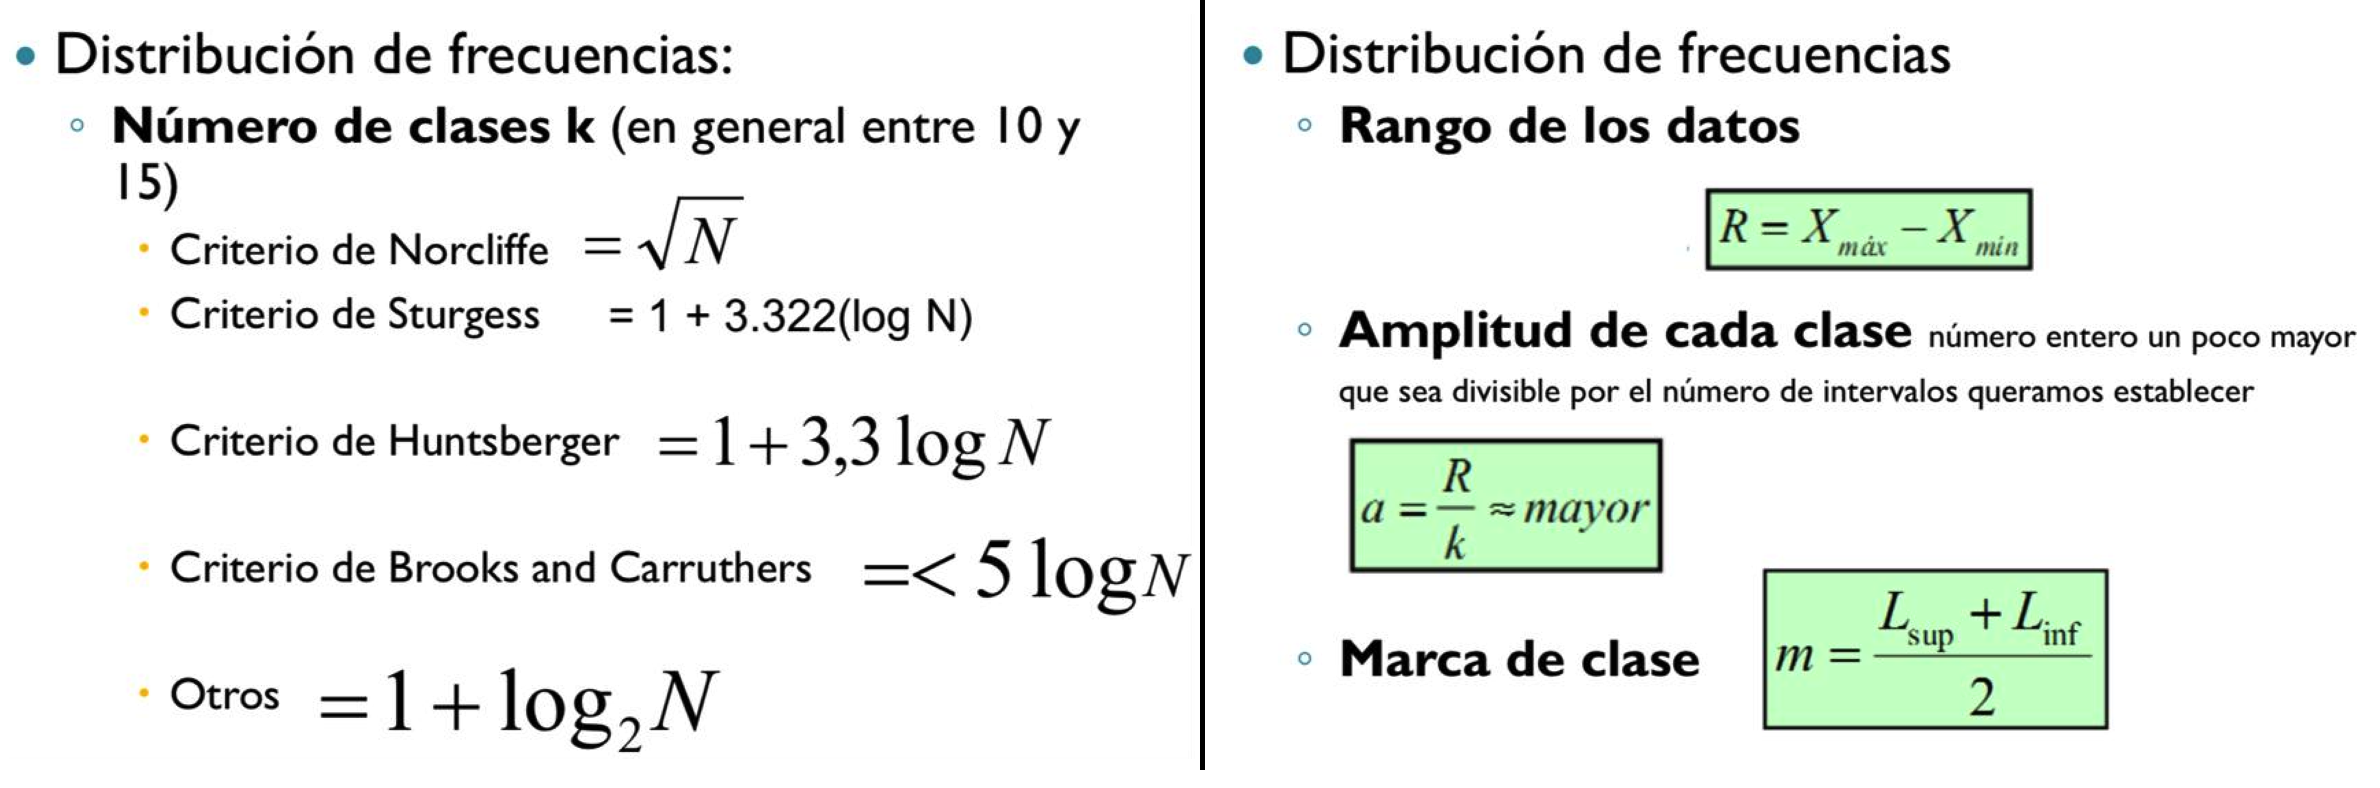
\includegraphics[width=1.05\textwidth]{imagenes/imagenes01/T01IM01.png}
		\end{figure}

Veamos un ejemplo:

\begin{example}. \label{ejparamedia}
	Las edades de un conjunto de niños son: 3, 7, 10, 10, 6, 5, 4.5, 12, 11, 10, 15, 10.5, 6, 2, 10, 9, 10, 4, 15, 13, 14, 12, 7, 10, 6, 8. Agrupando los datos, construir la tabla de frecuencias.
	
	\vspace{6mm} En los 26 datos hay 15 valores distintos (desde el 2 hasta el 15). Aplicando, p.e., el criterio de Norcliffe, tendremos que construir $\sqrt{15}\approx 4$ intervalos.
	
	\vspace{2mm}La amplitud de cada intervalo debe ser $\dfrac{15-2}{4}=\dfrac{13}{4}=3.25 \to 3.5 \text{ ó } 4$. Tomaremos $4$ como amplitud. Así, los intervalos en que agrupar los datos serán $[2,6[,\ [6,10[,\ [10,14[, \ [14,18[$
	
	\vspace{2mm}Distribuyendo, ahora, los datos en sus clases construimos la tabla de frecuencias.
	
	% Please add the following required packages to your document preamble:
% \usepackage{multirow}
\begin{table}[H]
\centering
\begin{tabular}{cr|r|rrr}
\multicolumn{1}{c|}{Edades}    & \multicolumn{1}{c|}{\multirow{2}{*}{\begin{tabular}[c]{@{}c@{}}Marcas\\ de clase\end{tabular}}} & \multicolumn{2}{c|}{Frecuencias}                        & \multicolumn{2}{c|}{F. acumuladas}                       \\ \cline{3-6} 
\multicolumn{1}{c|}{$x_i$}     & \multicolumn{1}{c|}{}                                                                             & \multicolumn{1}{c|}{$n_i$} & \multicolumn{1}{c|}{$f_i$} & \multicolumn{1}{c|}{$N_i$} & \multicolumn{1}{c|}{$F_i$}  \\ \hline
\multicolumn{1}{c|}{$[2,6[$}   & 4                                                                                                 & 5                          & \multicolumn{1}{r|}{5/26}  & \multicolumn{1}{r|}{5}     & \multicolumn{1}{r|}{5/26}  \\
\multicolumn{1}{c|}{$[6,10[$}  & 8                                                                                                 & 7                          & \multicolumn{1}{r|}{7/26}  & \multicolumn{1}{r|}{12}    & \multicolumn{1}{r|}{12/26} \\
\multicolumn{1}{c|}{$[10,14[$} & 12                                                                                                & 11                         & \multicolumn{1}{r|}{11/26} & \multicolumn{1}{r|}{23}    & \multicolumn{1}{r|}{23/26} \\
\multicolumn{1}{c|}{$[14,18[$} & 16                                                                                                & 3                          & \multicolumn{1}{r|}{3/26}  & \multicolumn{1}{r|}{26}    & \multicolumn{1}{r|}{26/26} \\ \cline{3-3}
                               &                                                                                                   & N=26                       &                            &                            &                            \\ \cline{3-3}
\end{tabular}
\end{table}
\end{example}

\textbf{Intervalos no solapados:} si los datos ya aparecen agrupados pero lo están en intervalos no solapados se tomarán intervalos que contengan a estos pero sin modificar las frecuencias.

Lo vemos con un ejemplo:

\begin{example}.
	% Please add the following required packages to your document preamble:
% \usepackage{multirow}
\begin{table}[H]
\centering
\begin{tabular}{c|ccc|c}
Internavo & $n_i$ & \multirow{5}{*}{$\quad \Rightarrow \quad$} & Intervalo   & $n_i$ \\ \cline{1-2} \cline{4-5} 
10 a 19   & 10    &                                            & [9.5,19.5[  & 10    \\
20 a 29   & 15    &                                            & [19.5,29,5[ & 15    \\
30 a 39   & 17    &                                            & [29.5,39,5[ & 17    \\
39 a 49   & 11    &                                            & [39.5,49.5[ & 17   
\end{tabular}
\end{table}
\end{example}

\section{Representaciones gráficas}


En los análisis estadísticos, es frecuente utilizar representaciones visuales complementarias de las tablas que resumen los datos de estudio. Con estas representaciones, adaptadas en cada caso a la finalidad informativa que se persigue, se transmiten los resultados de los análisis de forma rápida, directa y comprensible.

Cuando se muestran los datos estadísticos a través de representaciones gráficas, se ha de adaptar el contenido a la información visual que se pretende transmitir. Para ello, se barajan múltiples formas de representación. Los tipos más frecuentes de representaciones estadísticas son:

\begin{itemize}
	\item \textbf{Diagramas de barra}s: muestran los valores de las frecuencias absolutas sobre un sistema de ejes cartesianos, cuando el carácter estadístico en estudio es un atributos o  una variable discreta.
	\item \textbf{Histogramas}: formas especiales de diagramas de barras para distribuciones de variable continua.
	\item \textbf{Polígonos de frecuencias}: formados por líneas poligonales abiertas sobre un sistema de ejes cartesianos.
	\item \textbf{Gráficos de sectores}: circulares o de tarta, dividen un círculo en porciones proporcionales según el valor de las frecuencias relativas. \textcolor{gris}{Este tipo de diagramas no es nada recomendado.\footnote{Lo veremos más adelante, en su apartado correspondiente.}}
	\item \textbf{Pictogramas}: o representaciones visuales figurativas. En realidad son diagramas de barras en los que las barras se sustituyen con dibujos alusivos a la variable. 
	\item \textbf{Cartogramas}: expresiones gráficas a modo de mapa.
	\item \textbf{Pirámides de población}: para clasificaciones de grupos de población por sexo y edad.
\end{itemize}

\subsection{Diagrama de barras}

\begin{definition}
	. Un \textbf{diagrama de barras} es una representación gráfica en un eje cartesiano de las frecuencias de una variable cualitativa (atributo) o cuantitativa discreta.
		
	\vspace{2mm} Se representan, en el eje de abcisas, los valores de la serie estadística, y en el de ordenadas, los valores de las frecuencias absolutas.
	
	\vspace{2mm} Se suelen usar para comparar magnitudes de varias categorías, ver la evolución en el tiempo de una magnitud concreta, etc.
\end{definition}

\begin{example}

		\begin{figure}[H]
			\centering
			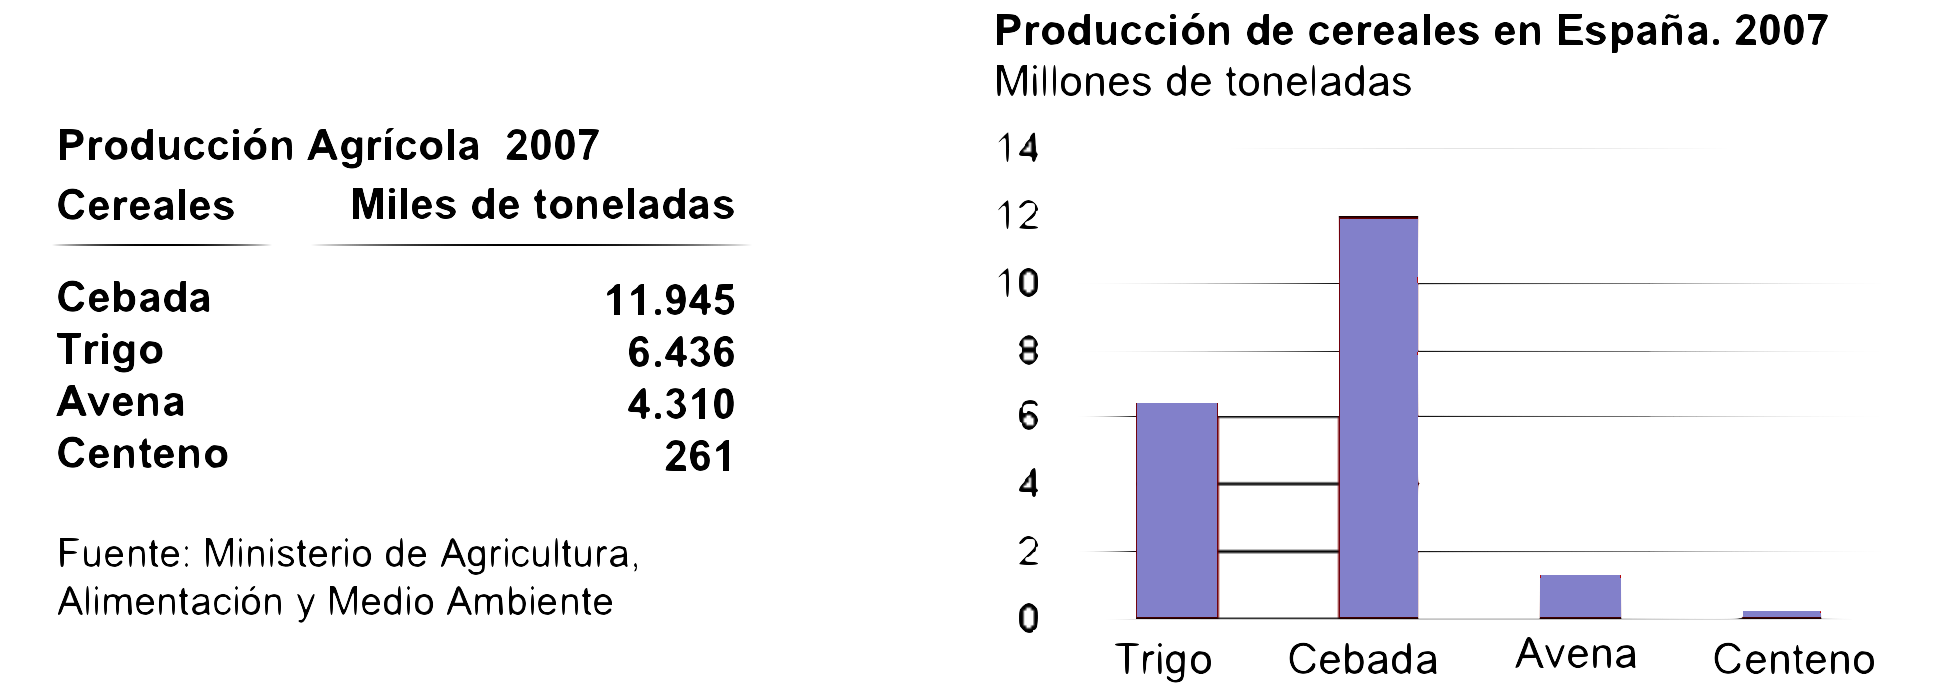
\includegraphics[width=1\textwidth]{imagenes/imagenes01/T01IM02.png}
			\caption*{\footnotesize{Diagrama de barras. (INE)}}
		\end{figure}
\end{example}

\subsection{Histogramas}
\begin{definition}
	. Los \textbf{histogramas} se usan para representar las frecuencias de una variable cuantitativa continua.

	\vspace{2mm} En uno de los ejes se posicionan las clases de la variable continua (los intervalos) y en el otro eje las frecuencias absolutas. No existe separación entre las barras.	
\end{definition}


\begin{example}

	\begin{figure}[H]
			\centering
			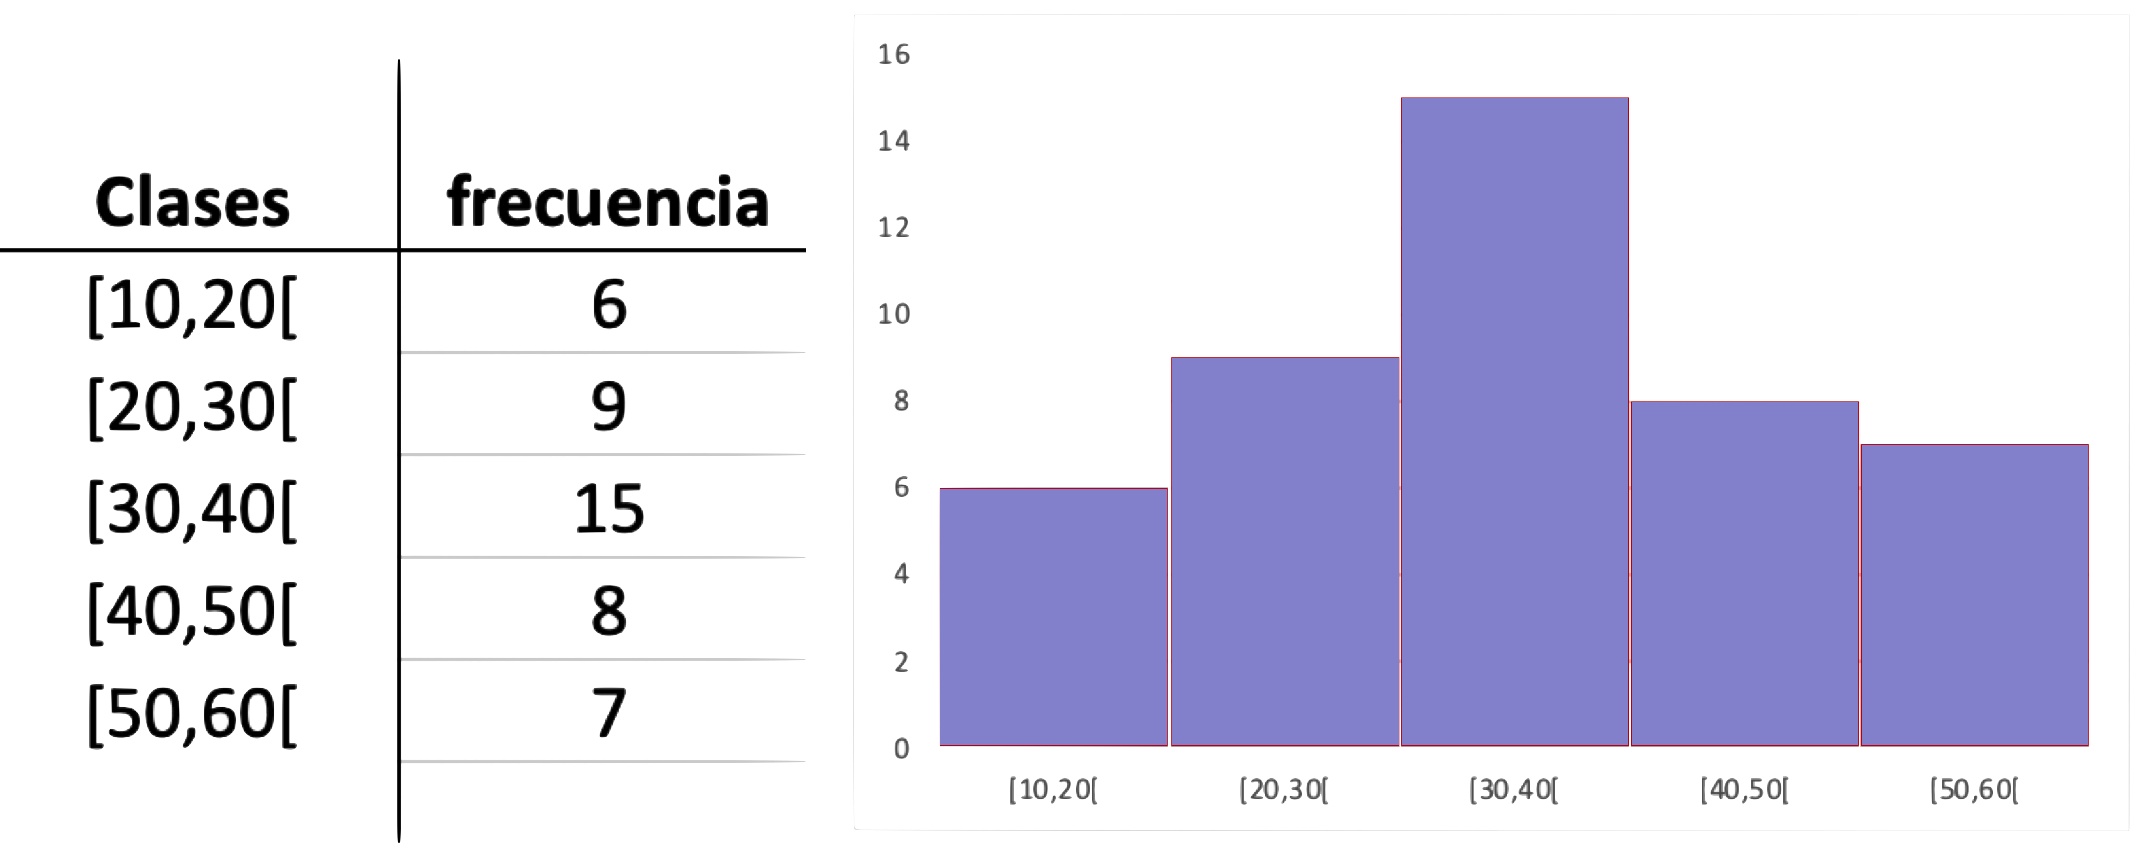
\includegraphics[width=.8\textwidth]{imagenes/imagenes01/T01IM03.png}
			\caption*{\footnotesize{Histograma.}}
		\end{figure}
\end{example}

\vspace{5mm}%**********************
\begin{example}

	Si las clases no son de la misma amplitud, no es la altura de los rectángulos sino su área el que debe ser proporcional a la frecuencia absoluta de cada una de ellas.

\begin{figure}[H]
			\centering
			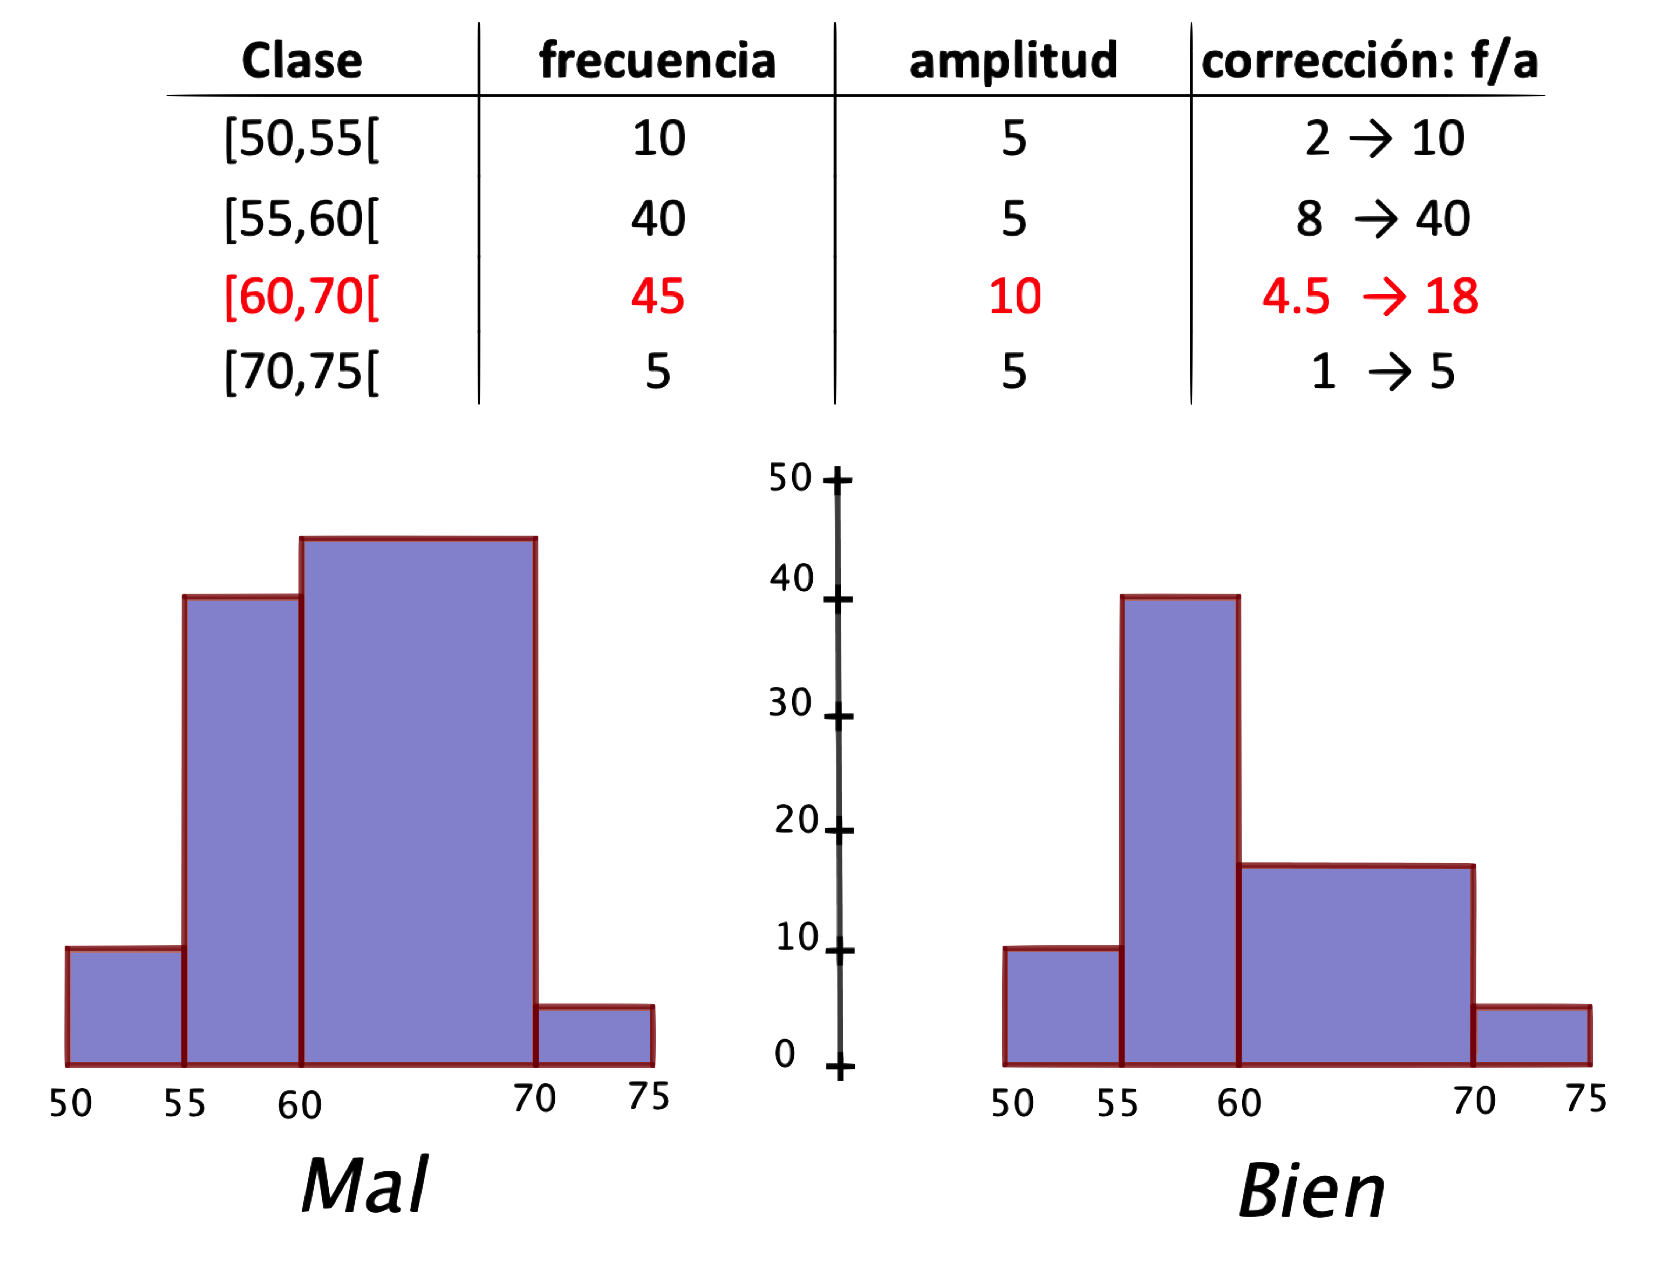
\includegraphics[width=.7\textwidth]{imagenes/imagenes01/T01IM04.png}
		\end{figure}

\end{example}



\subsection{Polígonos de frecuencias}

\begin{definition}
	. Un \textbf{polígono de frecuencias} es una linea poligonal que une o bien el extremos de las barras en un diagrama de barras o bien los puntos medios de las partes superiores de los rectángulos que forman un histograma	.
\end{definition}


\vspace{3cm} %*****************************************

\textcolor{white}{.}  %*****************************************

\vspace{3cm} %*****************************************

\begin{example}

\begin{figure}[H]
			\centering
			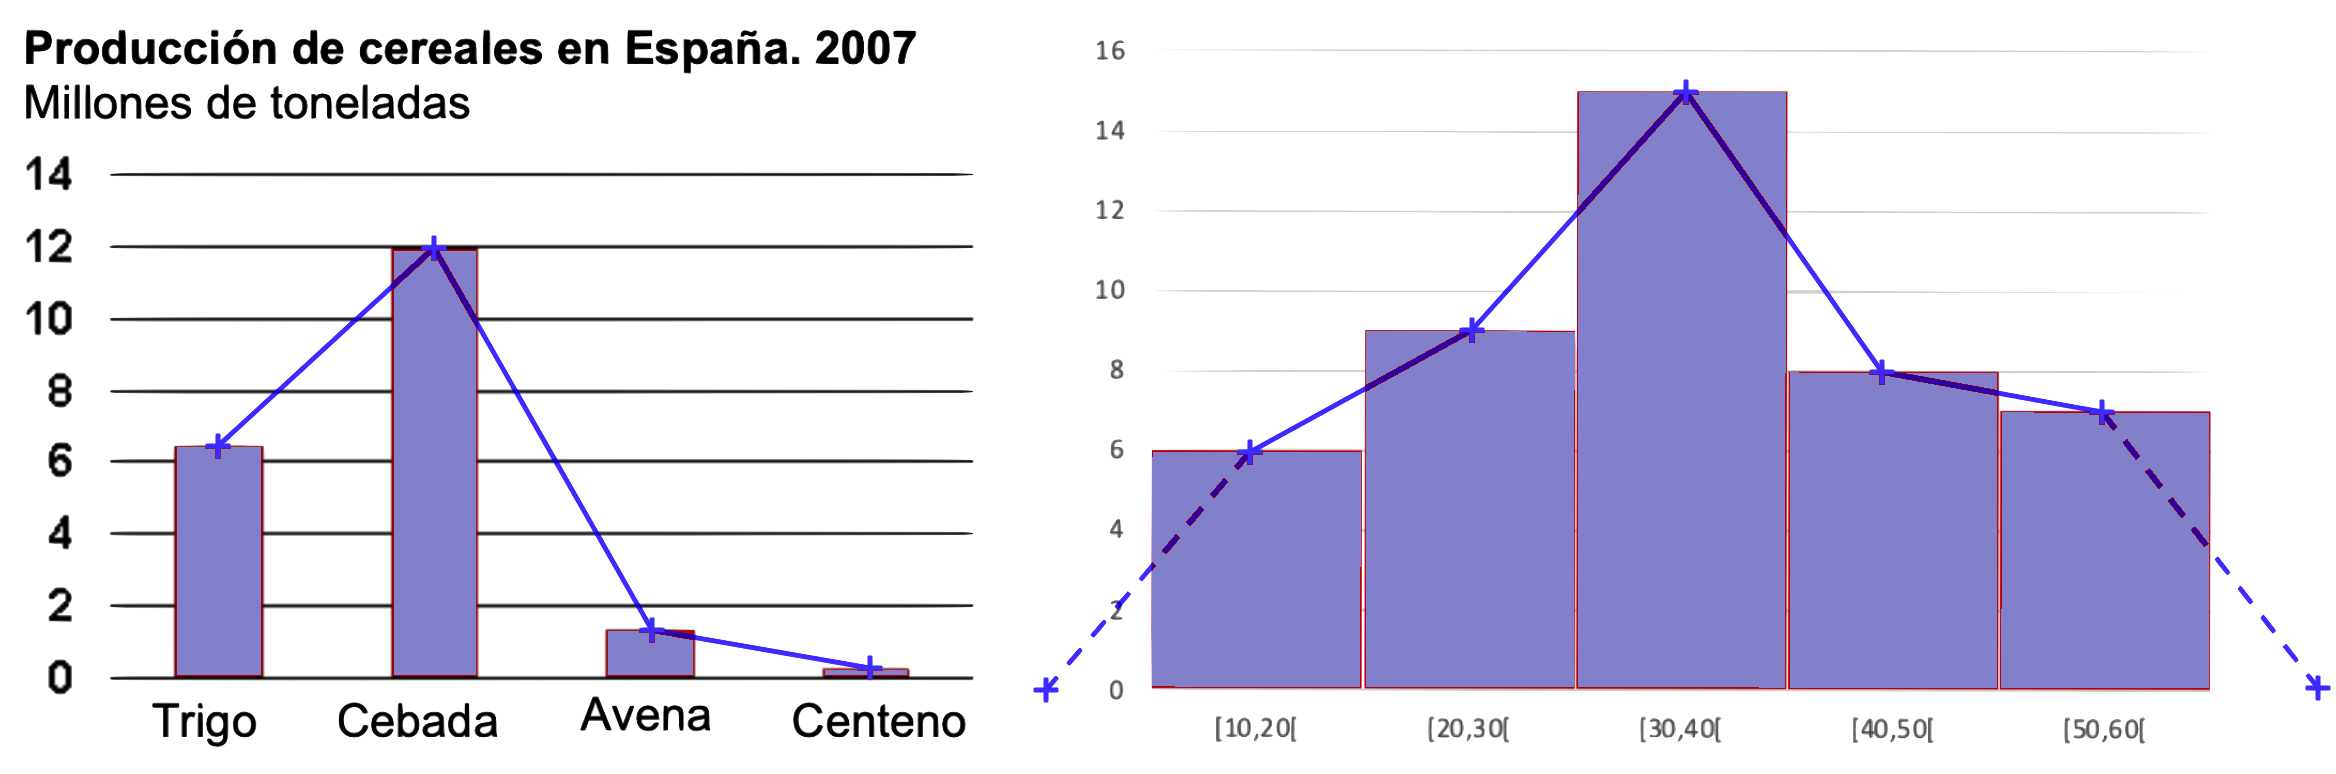
\includegraphics[width=1\textwidth]{imagenes/imagenes01/T01IM05.png}
			\caption*{\footnotesize{Polígonos de frecuencias (absolutas) en diagrama de barras y en histograma.}}
		\end{figure}


Si en lugar de usar en el eje de ordenadas las frecuencias absolutas se usan las frecuencias absolutas acumuladas, se obtienen los \emph{polígonos de frecuencias absolutas acumuladas}. También se habla de polígonos de frecuencias relativas y de frecuencias relativas acumuladas. 

El uso de este tipo de representaciones gráficas es muy útil para el cálculo aproximado de parámetros de posición, como veremos en el próximo apartado. 

\end{example}

\vspace{2cm} %*****************************************
\subsection{Diagrama de sectores}
\vspace{2cm} %*****************************************
\begin{definition}
	. En un \textbf{diagrama de sectores	},  la serie estadística se representa como sectores circulares de ángulo (área) proporcional a la frecuencia de cada dato.
	
	\vspace{2mm} Se suele usar para datos cualitativos y con pocos valores.
\end{definition}


\vspace{4cm} %*****************************************
\textbf{ \emph{``Tartas no, gracias''}}.

	\begin{figure}[H]
			\centering
			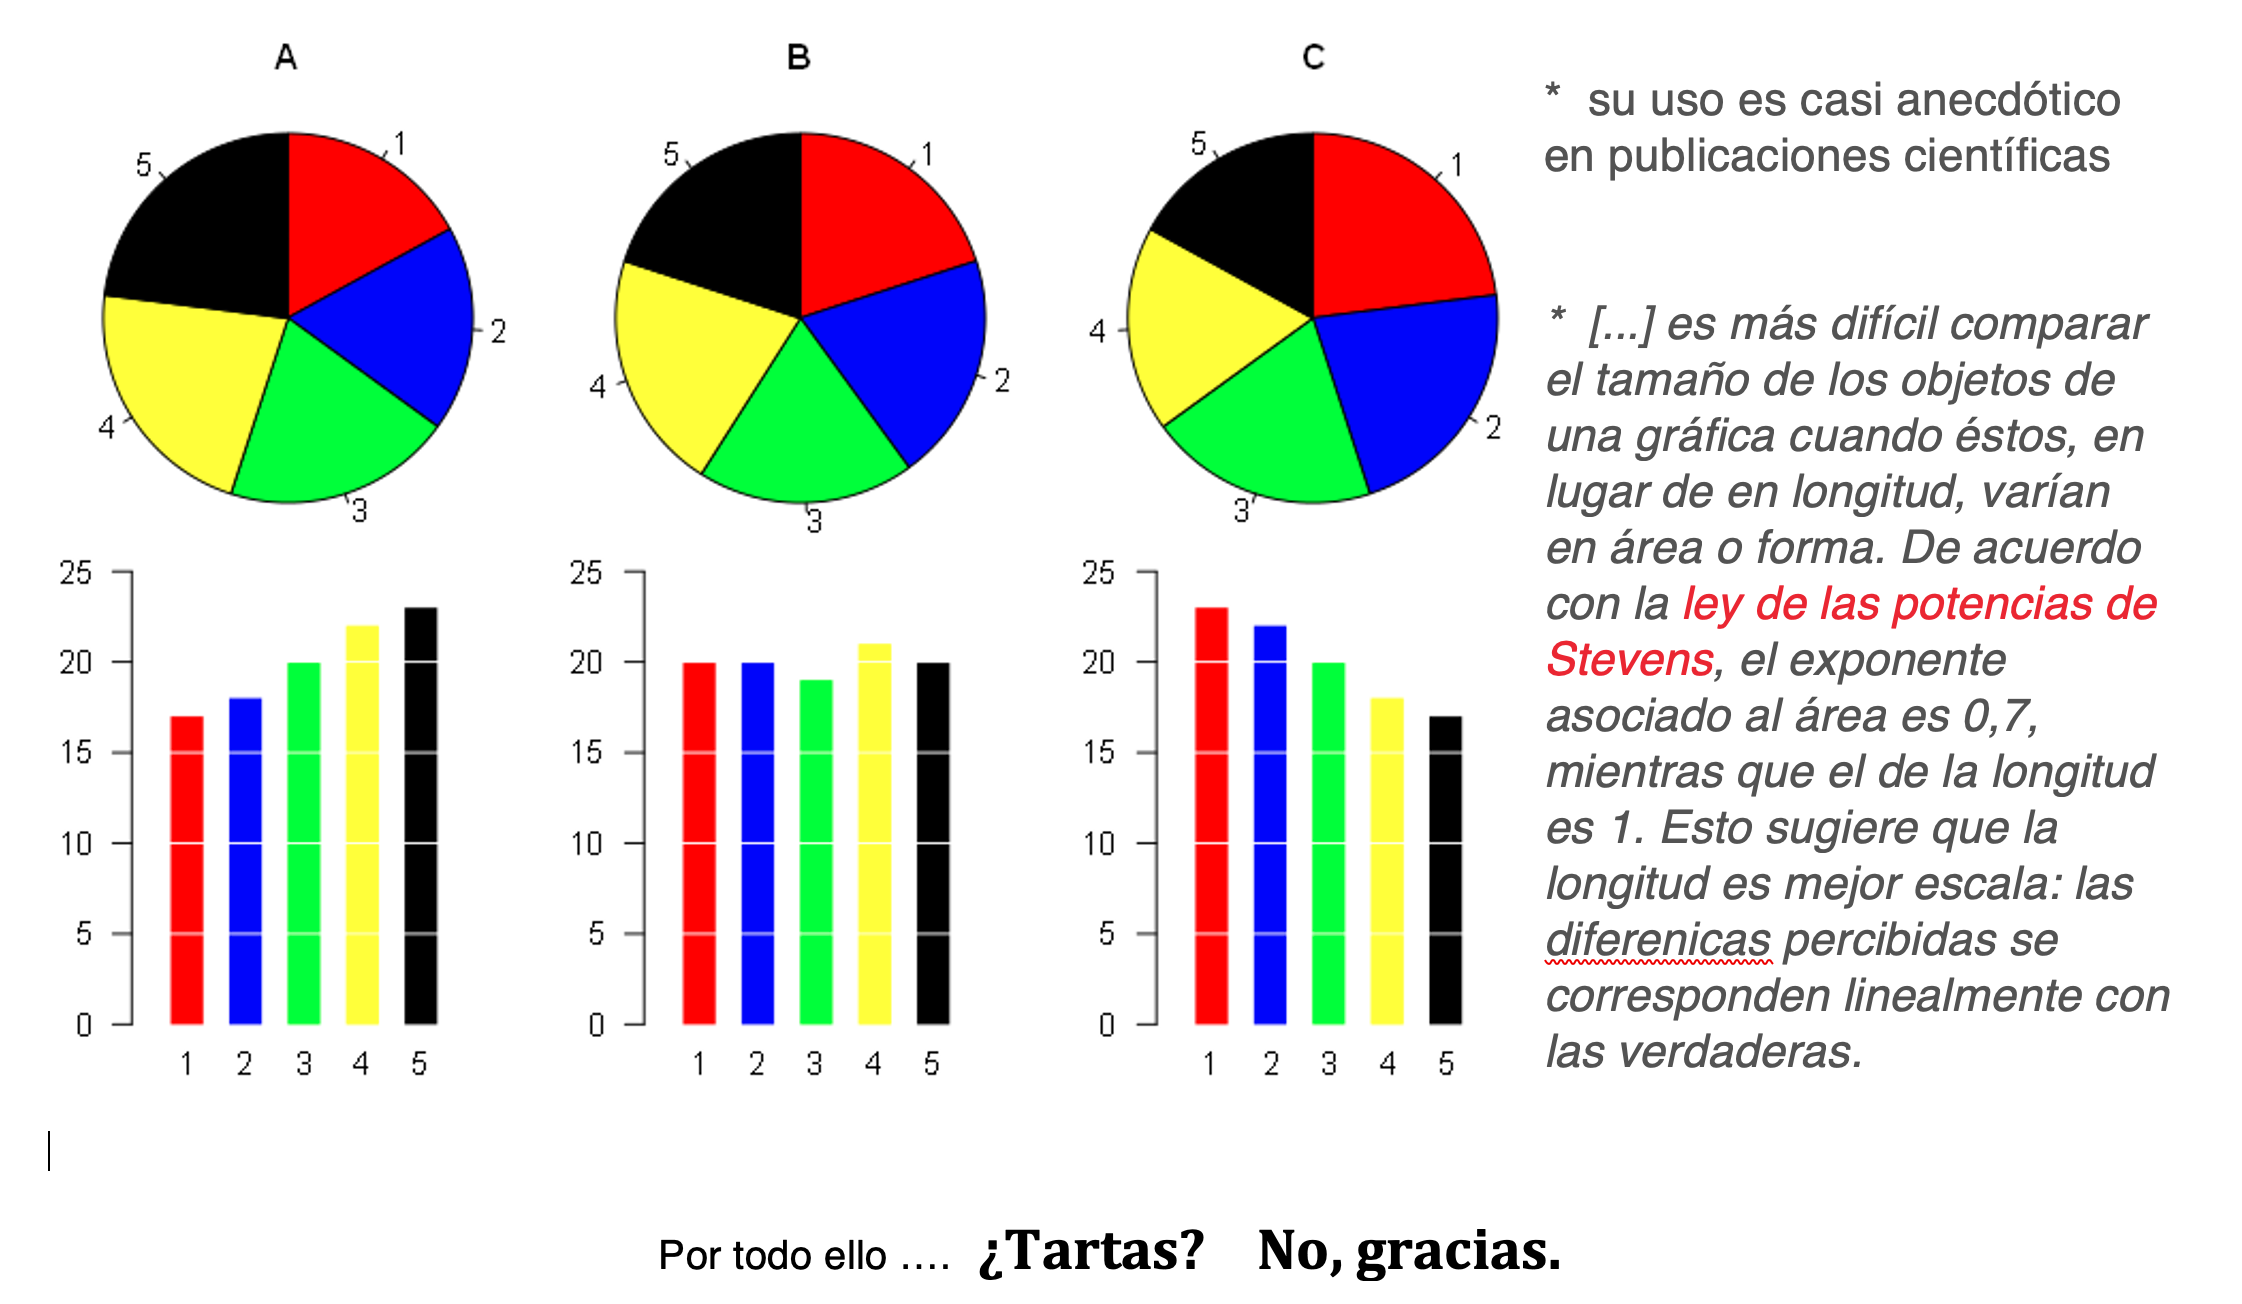
\includegraphics[width=1\textwidth]{imagenes/imagenes01/T01IM06.png}
			\caption*{\footnotesize{Los diagramas de sectores no son aconsejables.}}
		\end{figure}

	\begin{figure}[H]
			\centering
			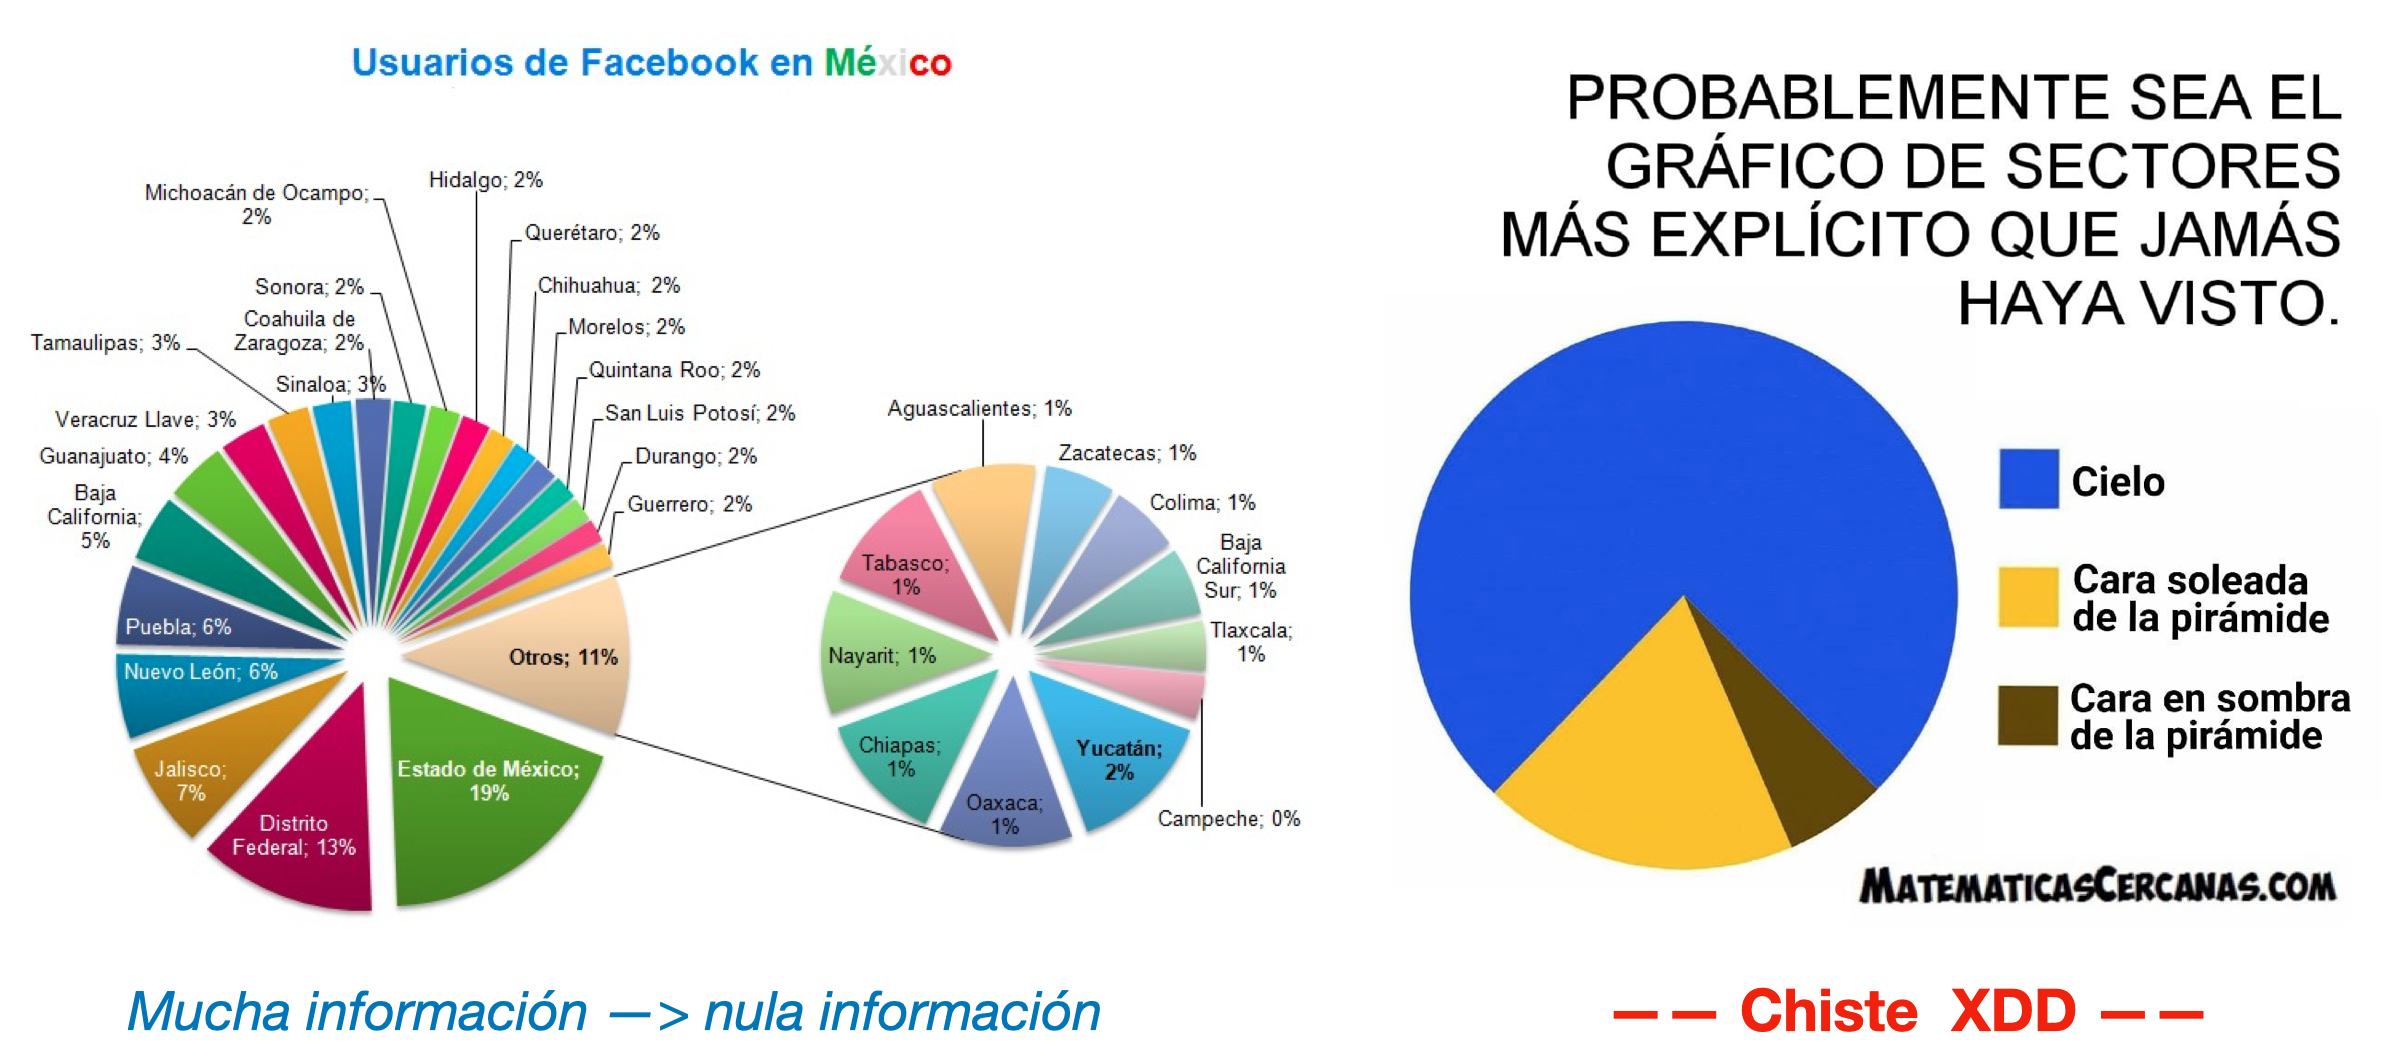
\includegraphics[width=1\textwidth]{imagenes/imagenes01/T01IM07.png}
		\end{figure}


\subsection{Otros tipos de representaciones gráficas en estadística}

	\begin{figure}[H]
			\centering
			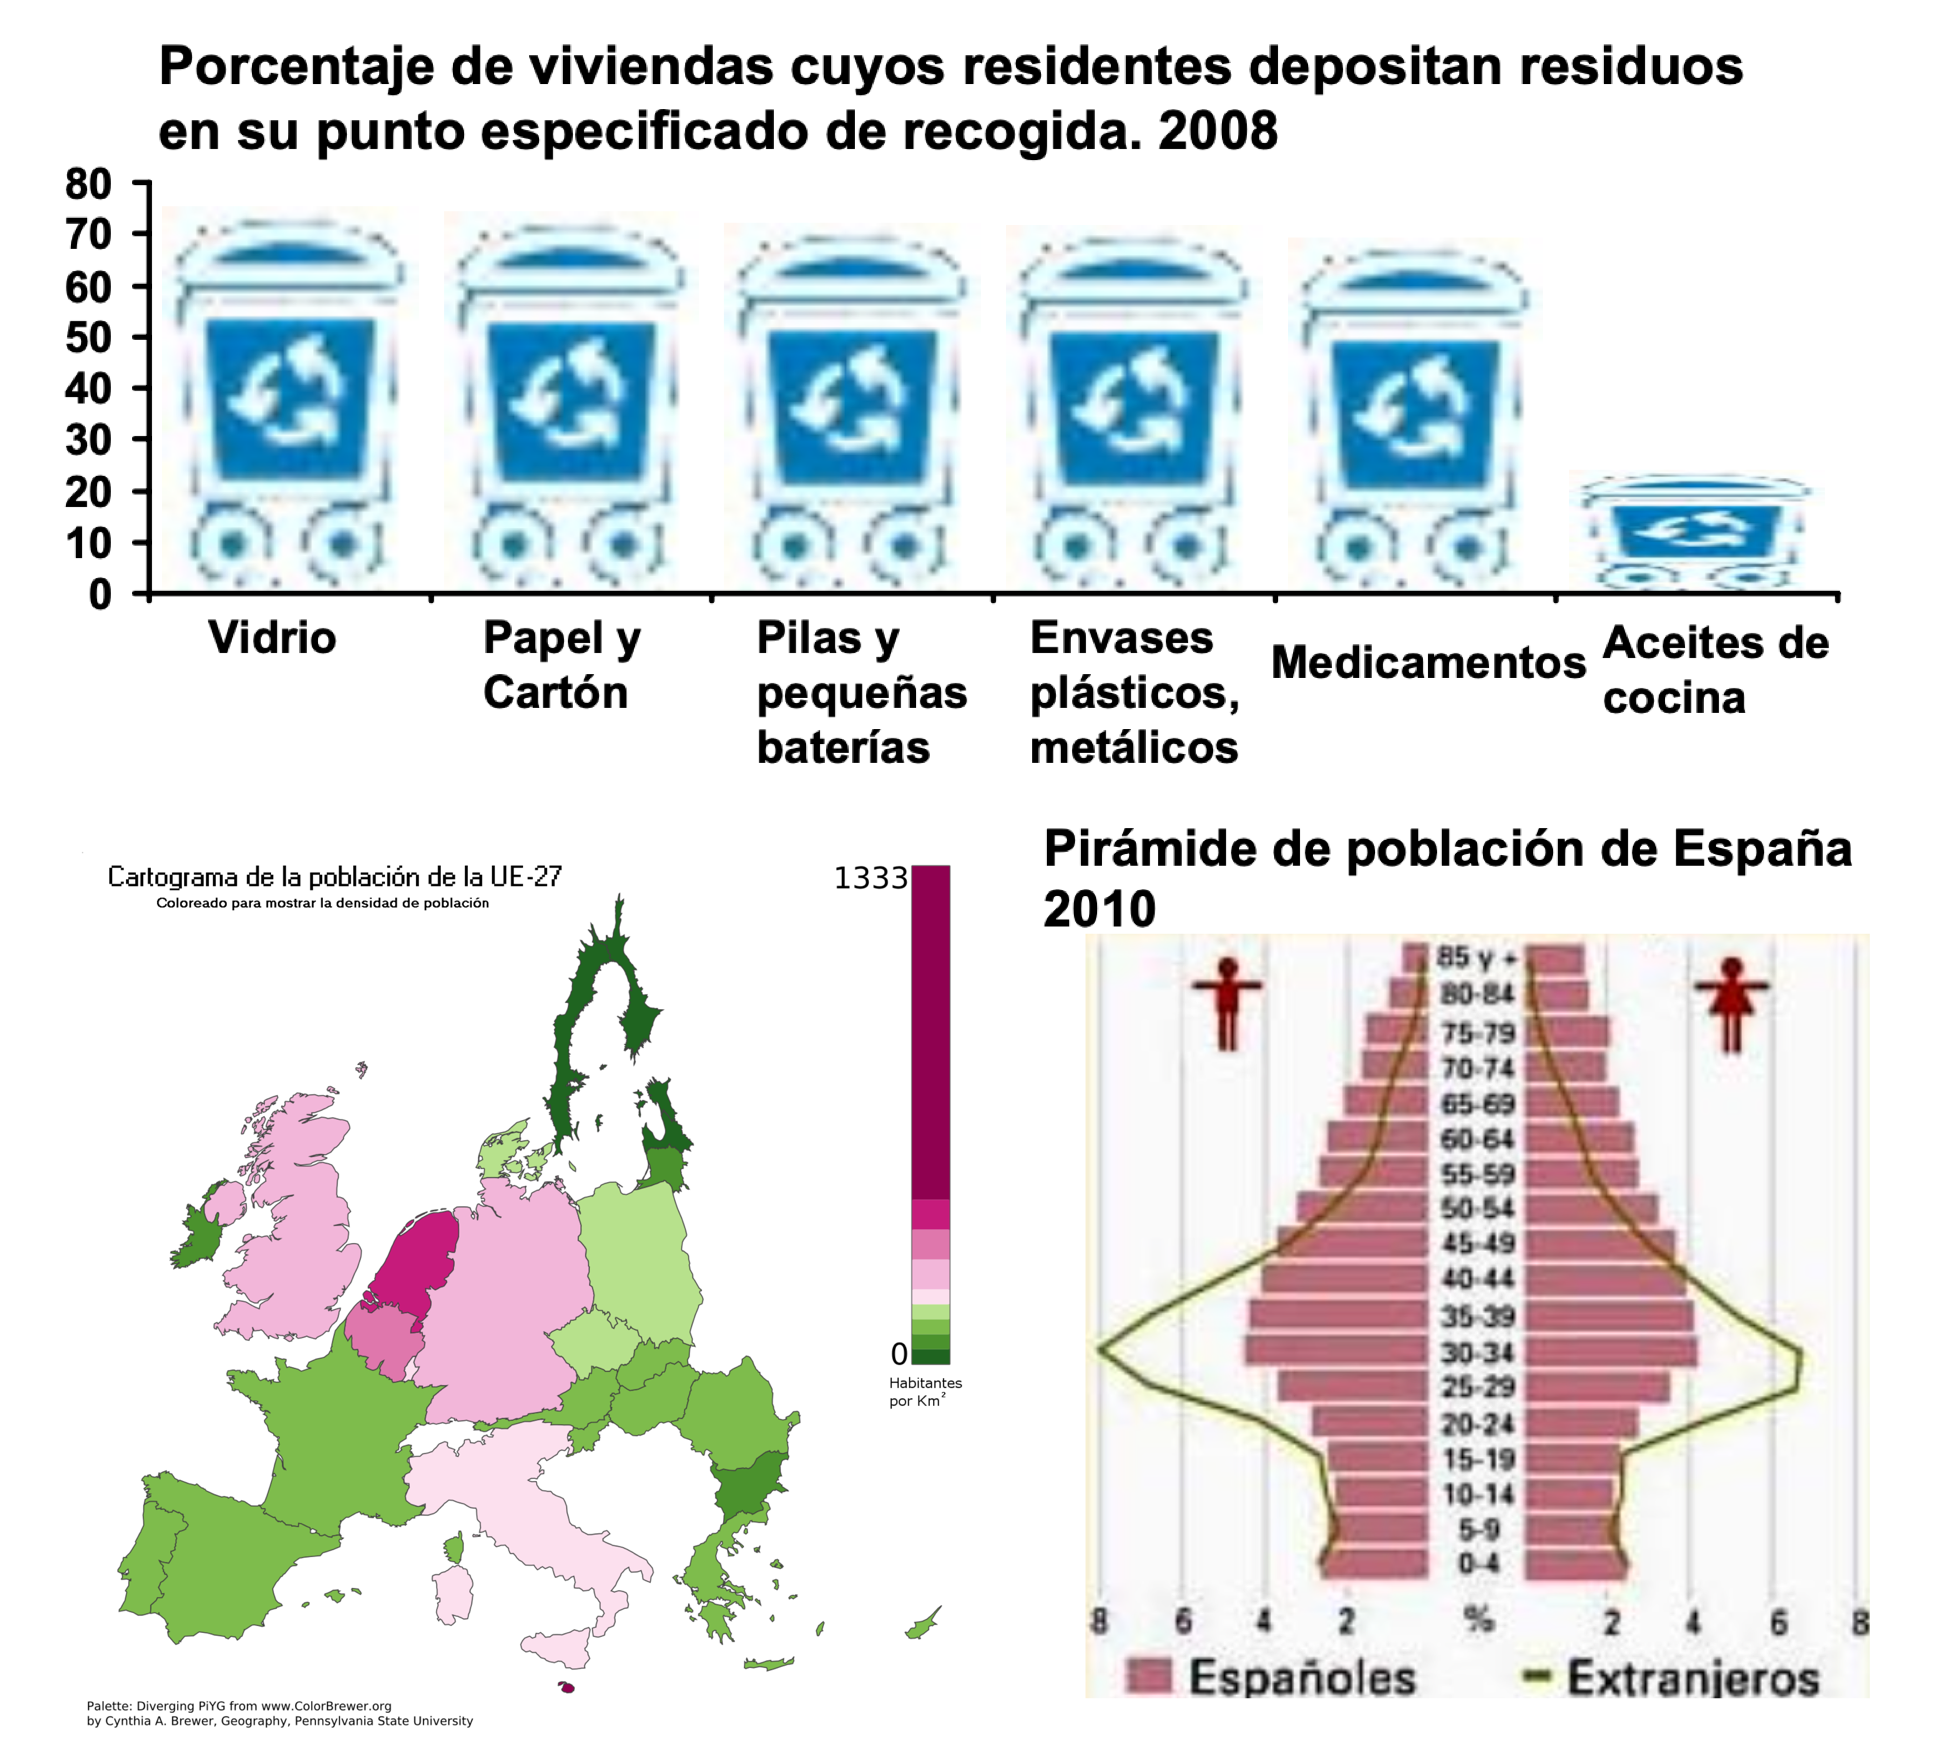
\includegraphics[width=.9\textwidth]{imagenes/imagenes01/T01IM08.png}
			\caption*{\footnotesize{Pictogramas, cartogramas y pirámides de población. (INE)}}
		\end{figure}

\begin{definition}
	. \textbf{Pictogramas}: se usan para datos no agrupados. Se representan con imágenes alusivas a la distribución y de tamaños proporcionales	(o repitiendo éstas un determinado número de veces) proporcional a la frecuencia. Tiene escasa precisión.
	
	\vspace{4mm} \textbf{Cartogramas}: se usan para representar sobre un mapa datos relacionados con un área geográfica.
	
	\vspace{4mm} \textbf{Pirámides de población}: son un par de histogramas verticales con un eje común, normalmente la edad y separando a izquierda y derecha por sexos.
	
\end{definition}



\subsection{Diagramas de tallos y hojas}

\begin{definition}
	. Un tipo de representación estadística que además es útil para el recuento de datos es el \textbf{diagrama de tallos y hojas} (Stem-and-Leaf Diagram) es un semigráfico que permite presentar la distribución de una variable cuantitativa. Consiste en separar cada dato en el último dígito (que se denomina hoja) y las cifras delanteras restantes (que forman el tallo).
\end{definition}


\vspace{5mm}%**********************

\begin{example}
	. Los datos siguientes corresponden a los tiempos de reacción de una muestra de $33$ sujetos, medidos en centésimas de segundo, son:
55, 51, 60, 56, 64, 56, 63, 63, 61, 57, 62, 50, 49, 70, 72, 54, 48, 53, 58, 66, 68, 45, 74, 65, 58, 61, 62, 59, 64, 57, 63, 52, 67.

\vspace{2mm} Construir el diagrama de tallos y hojas.

\begin{table}[H]
\centering
\begin{tabular}{c|ccccccccccccccc}
Tallos & \multicolumn{15}{l}{Hojas} \\ \hline
4 & 5 & 8 & 9 &  &  &  &  &  &  &  &  &  &  &  &  \\
5 & 0 & 1 & 2 & 3 & 4 & 5 & 6 & 6 & 7 & 7 & 8 & 8 & 9 &  &  \\
6 & 0 & 1 & 1 & 2 & 2 & 2 & 3 & 3 & 3 & 4 & 4 & 5 & 6 & 7 & 8 \\
7 & 0 & 2 & 4 &  &  &  &  &  &  &  &  &  &  &  & 
\end{tabular}
\end{table}
\end{example}


\subsection{Diagrama de cajas y bigotes}
Veremos este tipo de diagramas al final de la sección parámetros de posición.




\section{Parámetros estadísticos}

En los datos recogidos en tablas se pierde información si se agrupan en intervalos, aunque ello resulte necesario; aún se pierde más información al presentarlos en forma de gráficos pero se gana rapidez en la transmisión visual de la información. Pues, si lo que hacemos es asignar a toda la distribución estadística un limitado número de parámetros que la represente, la pérdida de la información es aún más grande pero inevitable para poder comparar rápidamente distintas distribuciones de datos, es lo que ocurre con los parámetros estadísticos.

Los parámetros estadísticos se dividen en:

\begin{adjustwidth}{20pt}{0pt}
\begin{itemize}
	\vspace{-2mm} \item Parámetros de centralización.
		\vspace{-2mm} \begin{itemize}
			\vspace{-1mm} \item Media aritmética (ponderada, geométrica, armónica).
			\vspace{-1mm} \item Moda.
			\vspace{-1mm} \item Mediana.
		\end{itemize}
	\vspace{-2mm} \item Parámetros de Posición.
		\begin{itemize}
			\vspace{-2mm} \item Cuartiles, Deciles, Percentiles.
		\end{itemize}
	\vspace{-2mm} \item Parámetros de dispersión.	
		\begin{itemize}
			\vspace{-1mm} \item Recorrido.
			\vspace{-1mm} \item Desviación media.
			\vspace{-1mm} \item Varianza. Desviación típica.
			\vspace{-1mm} \item Coeficiente de variación de Pearson.
		\end{itemize}
\end{itemize}
\end{adjustwidth}




\subsection{Parámetros de centralización}

\small{En matemáticas y estadística, una media o promedio es una medida de tendencia central. Resulta al efectuar una serie determinada de operaciones con un conjunto de números y que, en determinadas condiciones, puede representar por sí solo a todo el conjunto. Existen distintos tipos de medias, tales como la media geométrica, la media ponderada y la media armónica aunque en el lenguaje común, tanto en estadística como en matemáticas la elemental de todas ellas es el término que se refiere a la media aritmética.}

\vspace{5mm}%**********************
\begin{definition}
	. La \textbf{media aritmética} o simplemente media de una serie de valores aislados $\{x_1,x_2,\cdots , x_n\}$,  agrupados con sus frecuencias absolutas $\{n_1, n_2,\cdots n_n\}$, que se designa por $\boldsymbol{\bar{x}}$, se define como:

	
	$$\boxed{ \ \bold{ \bar{x}\ =\ \dfrac{x_1\cdot n_1+x_2\cdot n_2+\cdots +x_n \cdot n_n}{N}\ =\ \dfrac { \displaystyle \sum_{i=1}^n x_i\cdot n_i}{N} } \ }$$
donde $\ n_1+n_2+\cdots + n_n=\displaystyle \sum_{i=1}^n n_i=N \ $	 es el número total de datos.

\vspace{2mm} Si la distribución está agrupada en clases, $x_i$ representa a la \emph{`marca de clase'} o punto medio del intervalo.
\end{definition}

\vspace{5mm}%**********************
\begin{theorem}
	
	  \begin{enumerate}
 		\item La suma de las desviaciones respecto de la media es cero.
 		
 		$(x_1-\bar{x})\cdot n_1+ (x_2-\bar{x})\cdot n_2+\cdots +(x_n-\bar{x})\cdot n_n=0$
 		\item Si a cada valor de los datos $x_i$ se le añade una cantidad constante $b$, la media aumenta en $b$.
 		
 		$ \overline{ \{x_1+b, n_1;\ x_2+b,n_2; \ \cdots ; x_n+b, n_n \} } =\bar{x}+b$
 		\item Si a cada valor de los datos $x_i$ se le multiplica por una cantidad constante $a$, la media queda multiplicada por  $a$.
 		
 		$ \overline{ \{ax_1, n_1;\ ax_2,n_2; \ \cdots ; ax_n, n_n \} } =a\bar{x}$
 		
 		\item 	La media es \emph{`invariante'} frente a transformaciones lineales, cambio de origen y escala, de las variables; es decir si $X$ es una variable aleatoria e $Y$ es otra variable aleatoria que depende linealmente de $X$,  $\  Y = a\cdot X + b \ $ (donde $a$ representa la magnitud del cambio de escala y $b$ la del cambio de origen). De otro modo $\{x_i\}\to \{y_i=a\cdot x_i+b\}$ se tiene que:
 		
 		$\overline Y = a \cdot \overline X + b \qquad \text{ ó } \qquad \overline {\{y_i\}} = a \cdot \overline {\{x_i\}} + b$
 		
 		\end{enumerate}	
\end{theorem}

\begin{destacado}
Observaciones sobre la media aritmética:

\begin{adjustwidth}{20pt}{0pt}
\begin{itemize}
	
\item La media se puede hallar sólo para variables cuantitativas.
 
\item La media es independiente de las amplitudes de los intervalos.
 
\item La media es muy sensible a las puntuaciones extremas, también conocidos como valores atípicos.  

\item La media no se puede calcular si hay un intervalo con una amplitud indeterminada (clases abiertas, p.e. $[10,20[; \ [20,50[; \ \text{más de } 50$) ,  en este caso no es posible hallar la media porque no podemos calcular la marca de clase de último intervalo.	
\end{itemize}
\end{adjustwidth}
\end{destacado}


\begin{definition}
	. Otras medias:
	
	\textbf{Media ponderada}: $\ \bar{x_p}= \dfrac{\displaystyle \sum_{i_1}^N x_i\cdot p_i}{\displaystyle \sum_{i=1}^N p_i}; \qquad p_i \to \text{ pesos}$
	
	\vspace {3mm}  \small{A veces puede ser útil otorgar pesos o valores a los datos dependiendo de su relevancia para determinado estudio. Si a los valores $\{x_1,x_2,\cdots ,x_n\}$ se le conceden los pesos  $\{p_1,p_2,\cdots ,p_n\}$, la expresión anterior representa su `media ponderada'. Sirve para dar más peso a determinados valores.}
	
	\vspace{4mm} \textbf{Media Geométrica}: $\ \bar{x}_g=G= \displaystyle \sqrt[N]{x_1^{n_1} \cdot x_2^{n_2} \cdots x_n^{n_n}}$
	
	\vspace {3mm} \small{La media geométrica es un promedio muy útil en conjuntos de números que son interpretados en orden de su producto, no de su suma (tal y como ocurre con la media aritmética). Por ejemplo, las velocidades de crecimiento.}
	
	\vspace{4mm} \textbf{Media Armónica}: $\bar{x}_a=H=\dfrac{N} { \displaystyle \sum_{i=1}^n { \dfrac {n_i}{x_i} } } $
	
	\vspace {3mm} \small{La media armónica es un promedio muy útil en conjuntos de números que se definen en relación con alguna unidad, por ejemplo la velocidad (distancia por unidad de tiempo)}.
\end{definition}


\vspace{5mm}%**********************
\begin{example}
	. Cálculo de la media del ejemplo \ref{ejparamedia}:	
	
\begin{multicols}{2}
% Please add the following required packages to your document preamble:
% \usepackage{multirow}
\begin{table}[H]
\small
\centering
\begin{tabular}{cc|c|clc}
\cline{1-4}
\multicolumn{1}{|c|}{\textbf{edades}} & \textbf{$x_i$} & \textbf{$n_i$} & \multicolumn{1}{c|}{\textbf{$x_i\cdot n_i$}} & $\quad$ & \multirow{6}{*}{} \\ \cline{1-4}
\multicolumn{1}{c|}{[2,6[}            & 4              & 5              & 20                                           &         &                   \\
\multicolumn{1}{c|}{[6,10[}           & 8              & 7              & 56                                           &         &                   \\
\multicolumn{1}{c|}{[10,14[}          & 12             & 11             & 132                                          &         &                   \\
\multicolumn{1}{c|}{[14,18[}          & 16             & 3             & 48                                          &         &                   \\ \cline{3-4}
                                      &                & 26             & \multicolumn{1}{c|}{256}                     &         &                   \\ \cline{3-4}
\end{tabular}
\end{table}

\begin{center}
$\quad$

$\boldsymbol{\bar{x}=} \dfrac{\sum x_i\cdot n_i}{\sum n_i}=$

$=\dfrac{256}{26}=\boldsymbol{9.85}$
\end{center}

\end{multicols}
\end{example}

\vspace{5mm}%**********************
\begin{example}
	. Una empresa ha generado un 20 \% de rentabilidad el primer año, un 15 \% el segundo año, un 33 \% el tercer año y un 25 \% el cuarto año. Si  sumamos las cantidades y dividir entre cuatro, este valor no representa nada en correcto. Para calcular la media de varios porcentajes debemos hacer uso de la media geométrica. Aplicado al caso anterior, tendríamos lo siguiente:

\vspace{2mm}$\bar{x}_g=\sqrt[4]{1.20 \cdot 1.15 \cdot 1.33 \cdot 1.25}=1.23 \ \to \ 23 \%$ de beneficio medio en los cuatro años, es decir, si cada año hubiese ganado un 23 \%, hubiera ganado lo mismo que ganando un 20 \% el primer año, un 15 \% el segundo, un 33 \% el tercero y un 25 \% el último año.
\end{example}

\vspace{5mm}%**********************
\begin{example}
	. Un coche recorre $100 \ \mathrm{km}$ a una velocidad de $60 \ \mathrm{Km/h}$, otros $100 \ \mathrm{km}$ a 	$70 \ \mathrm{Km/h}$ y otros $100 \ \mathrm{km}$ a $80 \ \mathrm{Km/h}$. La velocidad media viene determinada por la \emph{media armónica}:
	
	\vspace{4mm} $\bar{x}_h=\dfrac{3}{\dfrac 1{60}+\dfrac 1{70} + \dfrac 1{80}}=69.04\ \mathrm{km/h} \quad $
	\begin{tiny}\textcolor{gris}{$\left( \text{velocidad media}=\dfrac{\text{espacio total}}{\text{tiempo empleado}} \right)$}\end{tiny}
\end{example}

\vspace{5mm}%**********************
\begin{definition}
	. Dada una serie estadística, se llama \textbf{moda}, \textbf{mo}, al valor de la serie que tiene mayor frecuencia absoluta.
	
	\vspace{2mm} Una serie estadística puede ser \emph{plurimodal} (tener más de una moda) y \emph{amodal}, sin moda (si todas las frecuencias son iguales).
\end{definition}

\vspace{5mm}%**********************
\begin{theorem}
	. La \textbf{moda para datos agrupados} se obtiene aplicando la fórmula:
	
	$$\boldsymbol{ mo=L_k+\dfrac{n_k-n_{k-1}}{(n_k-n_{k-1})+(n_k-n_{k+1})}\cdot c_k }\ ,\quad \text{ donde:}	$$
	
	\vspace{2mm} \begin{itemize}
	\vspace{-2mm} \item $L_k:\ $ extremo inferior de la \textbf{clase modal} (\emph{clase con mayor frecuencia absoluta})	.
	\vspace{-2mm} \item $n_k:\ $ frecuencia absoluta de la clase modal.
	\vspace{-2mm} \item $n_{k-1} \text{ y } n_{k+1}:\ $ frecuencias absolutas de las clases anterior y posterior a la clase modal.
	\vspace{-2mm} \item $c_k:\ $ amplitud de las clase modal.
	\end{itemize}

\end{theorem}

\vspace{5mm}%**********************
\begin{example}
	. Cálculo de la moda del ejemplo \ref{ejparamedia}:	
	
\begin{multicols}{2}
\small
\begin{table}[H]
\centering
\begin{tabular}{cc|c|}
\hline
\multicolumn{1}{|c|}{\textbf{edades}} & \textbf{$x_i$} & \textbf{$n_i$} \\ \hline
\multicolumn{1}{c|}{[2,6[}            & 4              & 5              \\
\multicolumn{1}{c|}{[6,10[}           & 8              & 7              \\
\multicolumn{1}{c|}{[10,14[}          & 12             & 11             \\
\multicolumn{1}{c|}{[14,18[}          & 16             & 3             \\ \cline{3-3} 
                                      &                & 26             \\ \cline{3-3} 
\end{tabular}
\end{table}
\textbf{Intervalo modal:} $\boldsymbol{ [10,14[ }$

$n_i=n_3=11;\ n_{i-1}=n_2=7;\ n_{i+1}=n_4=3$

$L_i=L_3=10;\ c_i=4$

$mo=10+\dfrac{(11-7)}{(11-7)+(11-3)}\cdot 4$

$mo=11.33$

\end{multicols}
	
En muchas ocasiones es suficiente con determinar el intervalo modal (el de mayor frecuencia absoluta).
\end{example}

\vspace{5mm}%**********************
\begin{definition}
	. Dada una serie estadística de un \emph{número impar de valores}, se llama \textbf{mediana} , \textbf{me}, al valor central de la serie, es decir, aquel valor tal que	 la mitad de los valores son mayores o iguales a él y la otra mitad, menores o iguales a él. Suponiendo la serie estadística \emph{ordenada en sentido creciente}.
	
	\vspace{2mm} Si la serie tiene un \emph{número par de valores}, se define la media como la \emph{semisuma de los dos valores centrales}.
\end{definition}

Para un determinado número de individuos $N$, el valor central viene determinado por $ \frac{N+1}{2}$. Si el resultado es decimal, hay dos individuos centrales, el  $\frac{N}{2}$ y el $\frac N 2 + 1$.

\vspace{5mm}%**********************
\begin{theorem}
	. Para datos agrupados, si la media está en la clase $[L_k,L_{k+1}[$, de frecuencia absoluta $n_k$, frecuencia absoluta acumulada de la clase anterior a la mediana $N_{k-1}$ y de  $c_i$  amplitud de la clase mediana, la \textbf{mediana} la determina la fórmula:	
	
	$$\boldsymbol{ me=L_k+\dfrac{\dfrac N 2 - N_{k-1}}{n_{k}}\cdot c_k }$$
\end{theorem}


\vspace{5mm}%**********************
\begin{example}
. --- En la serie: $2,4,6,\boldsymbol{8},9,10,12$, la mediana es $\ me=8$

\vspace{2mm} --- En la serie: $2,2,3,\boldsymbol{5}, \boldsymbol{8}, 10, 10, 12$, la mediana es $\ me=\dfrac{5+8}{2}=6.5$

\vspace{2mm} --- En la serie del ejemplo \ref{ejparamedia}, la mediana será:

\begin{multicols}{2}
\begin{table}[H]
\small
\centering
\begin{tabular}{cc|c|cc}
\cline{1-4}
\multicolumn{1}{|c|}{\textbf{edades}} & \textbf{$x_i$} & \textbf{$n_i$} & \multicolumn{1}{c|}{\textbf{$N_i$}} & \textcolor{gris}{$H_i$} \\ \cline{1-4}
\multicolumn{1}{c|}{[2,6[}            & 4              & 5              & 5                                   & \textcolor{gris}{0.19}  \\
\multicolumn{1}{c|}{[6,10[}           & 8              & 7              & 12                                  & \textcolor{gris}{0.46}  \\
\multicolumn{1}{c|}{[10,14[}          & 12             & 11             & 23                                  & \textcolor{gris}{0.88}  \\
\multicolumn{1}{c|}{[14,18[}          & 12             & 3              & 26                                  & \textcolor{gris}{1.00}  \\ \cline{3-3}
                                      &                & 26             &                                     &       \\ \cline{3-3}
\end{tabular}
\end{table}
$\dfrac N 2=13; \ L_k=10,$

$n_k=11; \ N_{k-1}=12$

$k=3$,  clase mediana $[10,14[$

$\quad$

$me=10+\dfrac{13-12}{10}\cdot 4=10.36$

\end{multicols}
En ocasiones es suficiente con determinar la clase mediana.
\end{example}

Se puede obtener un valor aproximado de la mediana a través del histograma de frecuencias relativas acumuladas \textcolor{gris}{(ahora, la línea poligonal no une los puntos medios de cada clase sino los extremos superiores de cada clase)}.

	\begin{figure}[H]
			\centering
			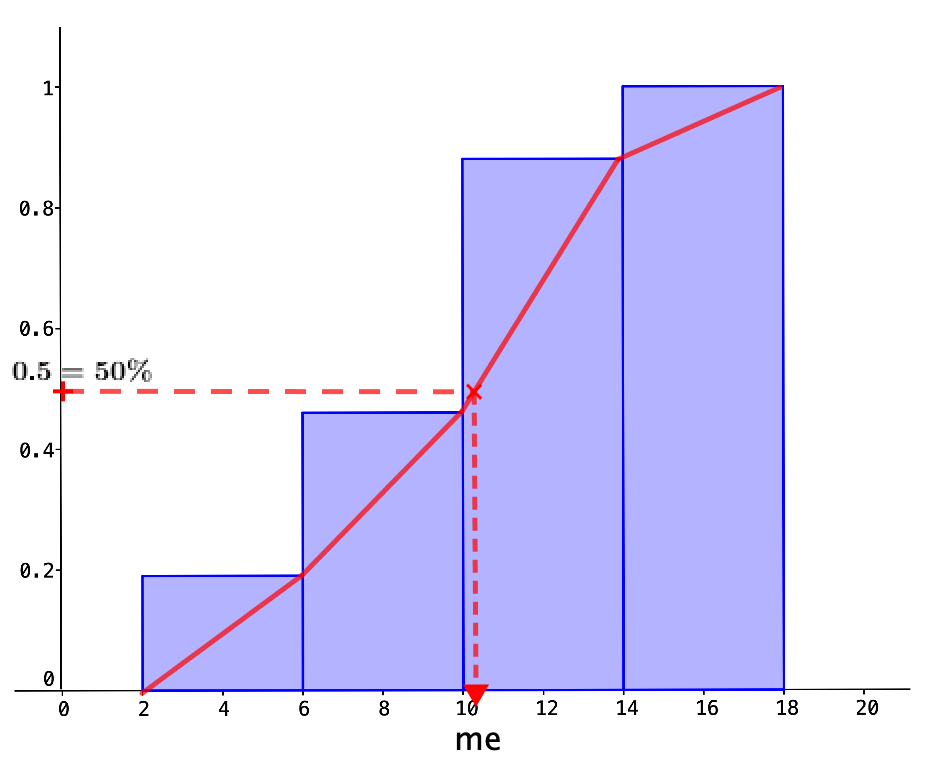
\includegraphics[width=.75\textwidth]{imagenes/imagenes01/T01IM09.png}
		\end{figure}

Tanto en el caso de la mediana como en el de la moda para datos agrupados, las fórmulas se deducen la una \emph{simple interpolación lineal}.


\begin{figure}[H]
			\centering
			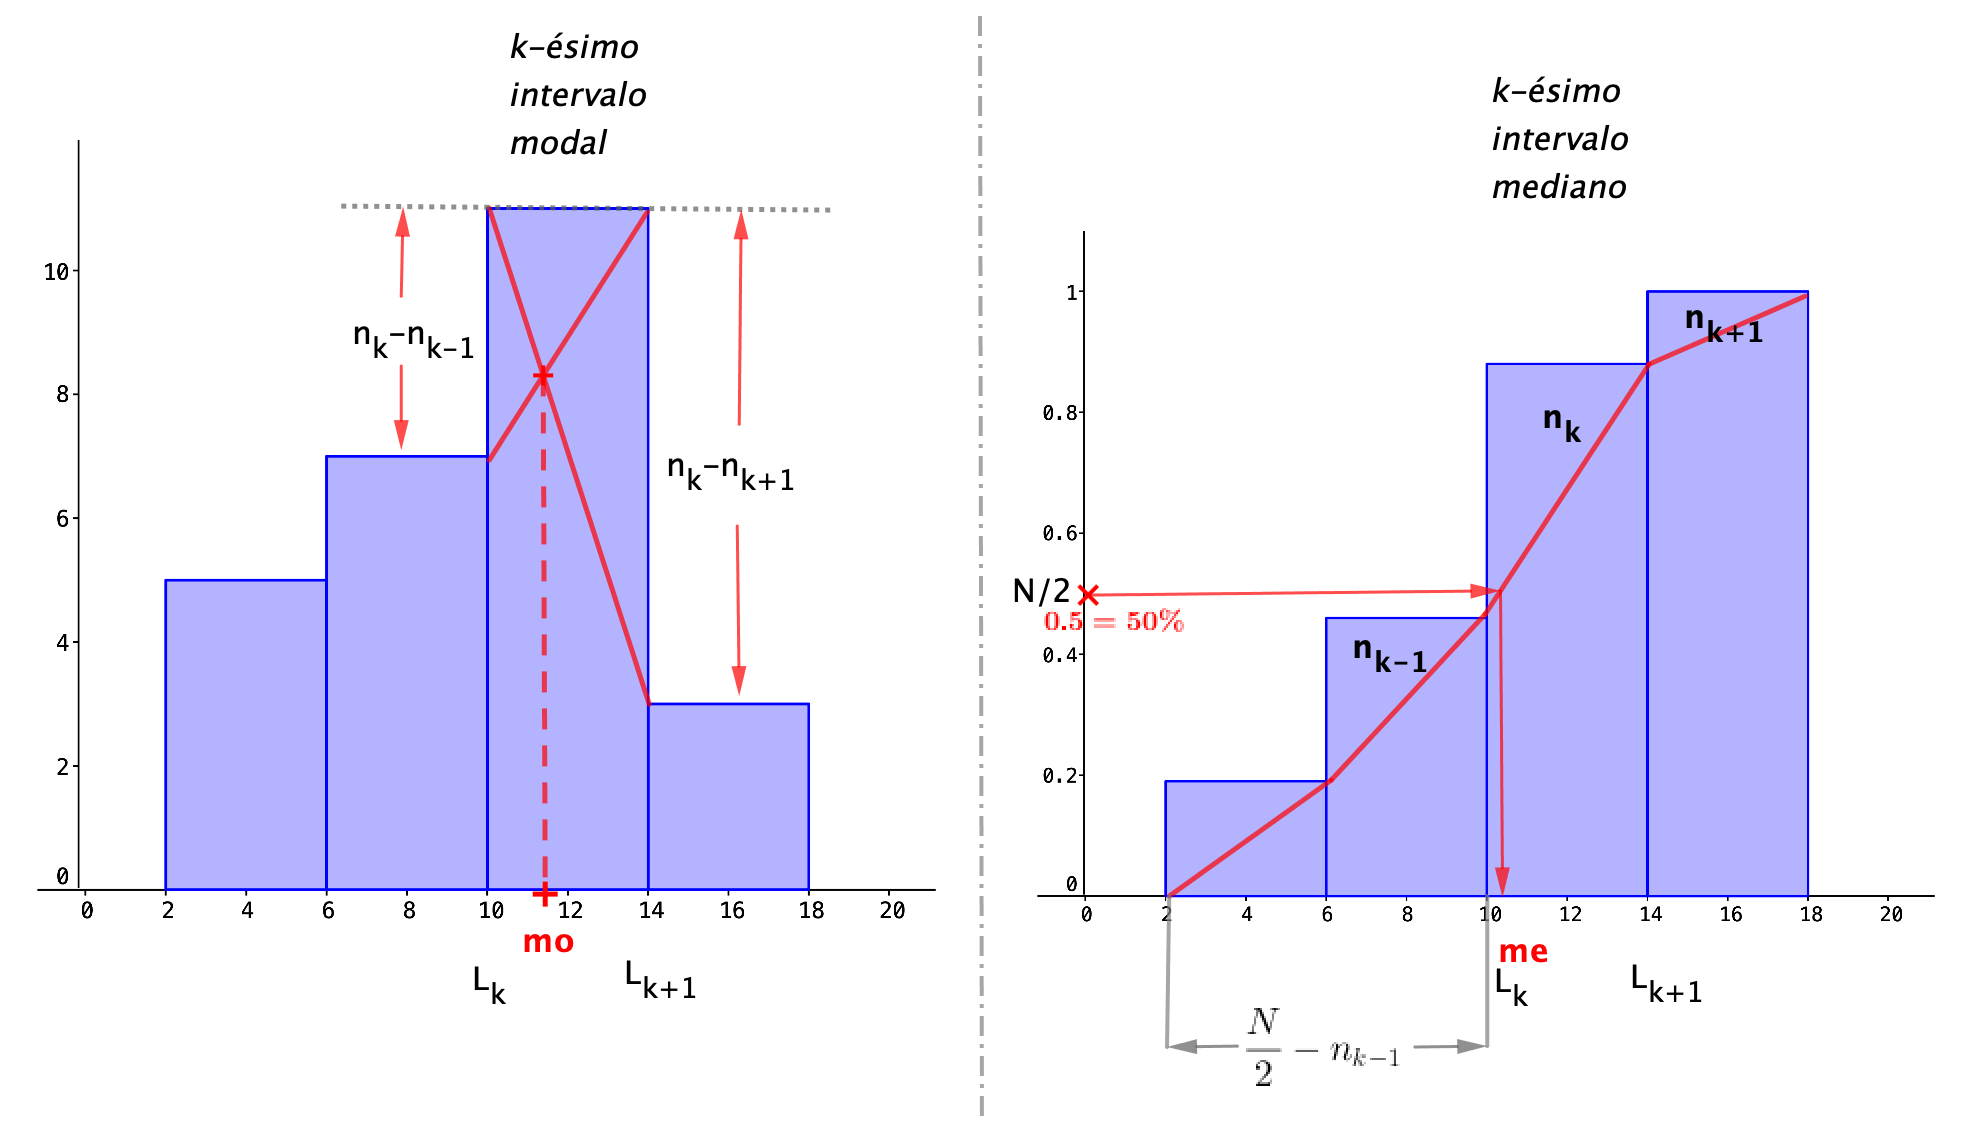
\includegraphics[width=1.05\textwidth]{imagenes/imagenes01/T01IM10.png}
		\end{figure}


\vspace{5mm}%**********************		
\begin{ejemplo}
	
\begin{ejre}

Calcular Media, moda y mediana para la siguiente serie estadística.

\begin{multicols}{2}
\begin{footnotesize}
\begin{table}[H]
\small
\centering
\begin{tabular}{rr|r|r|r}
\hline
\multicolumn{1}{|c|}{\textbf{Clases}} & \multicolumn{1}{c|}{\textbf{$x_i$}} & \multicolumn{1}{c|}{\textbf{$n_i$}} & \multicolumn{1}{c|}{\textbf{$N_i$}} & \multicolumn{1}{c|}{\textbf{$x_i\cdot n_i$}} \\ \hline
\multicolumn{1}{r|}{[20,30[}          & 25                                  & 20                                  & 20                                  & 500                                          \\
\multicolumn{1}{r|}{[30,40[}          & 35                                  & 35                                  & 25                                  & 1225                                         \\
\multicolumn{1}{r|}{[40,50[}          & 45                                  & 50                                  & 105                                 & 2250                                         \\
\multicolumn{1}{r|}{[50,60[}          & 55                                  & 49                                  & 154                                 & 2695                                         \\
\multicolumn{1}{r|}{[60,70[}          & 65                                  & 25                                  & 179                                 & 1625                                         \\
\multicolumn{1}{r|}{[70,80[}          & 75                                  & 15                                  & 194                                 & 1125                                         \\
\multicolumn{1}{r|}{[80,90[}          & 85                                  & 6                                   & 200                                 & 510                                          \\ \cline{3-3} \cline{5-5} 
                                      &                                     & 200                                 &                                     & \multicolumn{1}{r|}{9930}                    \\ \cline{3-3} \cline{5-5} 
\end{tabular}
\end{table}
\end{footnotesize}
\hspace{1cm} \begin{footnotesize}$\bar{x}=\dfrac{9930}{200}$\end{footnotesize}

\hspace{1cm} $\boldsymbol{ \bar{x}=49.65 }$

\hspace{1cm} \begin{scriptsize}$mo=40+\dfrac{50-35}{(50-35)+(50-49)} 10$\end{scriptsize}

\hspace{1cm} $\boldsymbol{ mo=49.38 }$

\hspace{1cm} \begin{footnotesize}$me=40+\dfrac{\dfrac{200}{2}-55}{50}\cdot 10$\end{footnotesize}

\hspace{1cm} $\boldsymbol{ me=49.00 }$

\end{multicols}

\end{ejre}
\end{ejemplo}


\vspace{10mm}%**********************
\begin{myalertblock}{Ventajas y desventajas de la medidas de tendencia central.}

%\begin{footnotesize}
\begin{itemize}

\item MEDIA

	\begin{itemize}
	\item Ventajas 
		\begin{itemize}
		\item Es la medida de tendencia central más usada.
		\item Emplea en su cálculo toda la información disponible.
		\item Es un valor único.
		\item Se emplea a menudo en cálculos estadísticos posteriores.
		\item Tiene un sentido claro como valor de tendencia del agrupamiento de los datos.
		\item Es sensible a cualquier cambio en los datos (puede ser usado como un detector de variaciones en los datos).
		\item Es útil para llevar a cabo procedimientos estadísticos como la comparación de medias de varios conjuntos de datos.
		\item Presenta rigor matemático.
		\item En la gráfica de frecuencia representa el centro de gravedad.
		\end{itemize}
	\item Desventajas
		\begin{itemize}
		\item Es sensible a los valores extremos.
		\item No es recomendable emplearla en distribuciones muy asimétricas.
		\item Si se emplean variables discretas, la media aritmética puede no pertenecer al conjunto de valores de la variable.
		\item No se puede calcular para datos cualitativos.
		\item No se puede calcular para datos que tengan clases de extremo abierto, tanto superior como inferior.
		\end{itemize}
	\end{itemize}

\item MEDIANA
	\begin{itemize}
	\item Ventajas:
		\begin{itemize}
		\item No se ve influenciada por valores extremos, ya que solo influyen los valores centrales.
		\item Fácil de entender.
		\item Se puede calcular para cualquier tipo de datos cuantitativos, incluso los datos con clase de extremo abierto.
		\item Es la medida de tendencia central más representativa en el caso de variables que solo admiten la escala ordinal.
		\end{itemize}
	\item Desventajas
		\begin{itemize}
		\item No utiliza en su cálculo toda la información disponible.
		\item No pondera cada valor por el número de veces que se ha repetido.
		\item Hay que ordenar los datos antes de determinarla.
		\end{itemize}
	\end{itemize}

\item MODA
	\begin{itemize}
		\item Ventajas
		\begin{itemize}
		\item No requiere cálculos.
		\item Puede usarse para datos tanto cuantitativos como cualitativos.
		\item Fácil de interpretar.
		\item No se ve influenciada por valores extremos.
		\item Se puede calcular en clases de extremos abiertos.
		\end{itemize}
	\item Desventajas
		\begin{itemize}
		\item Solo tiene significado en el caso de una gran cantidad de datos.
		\item No utiliza toda la información disponible.
		\item Difícil de interpretar si los datos tiene 3 o más modas.
		\end{itemize}
	\end{itemize}

\end{itemize}
%\end{footnotesize}
	
\end{myalertblock}


\vspace{5mm}%**********************
\begin{myexampleblock}{?`Cuál de los parámetros de posición es más representativo?}
\begin{small}

Cuando estudiamos las medidas de tendencia central, como la media, la moda y la mediana, nos preguntamos, tantas medidas y al final,  ?`cuál es la mas representativa?, ?`es suficiente con las medidas de tendencia central para caracterizar a un conjunto de datos?\footnote{Del blog  ``https://estadisticaestasahi.blogspot.com’’}


\vspace{2mm} Aclaremos esto con un ejemplo (tomado de ``Probabilidades y Estadística. Su Enseñanza’’ de J. Foncuberta, Red Federal de Formación Docente Continua, MECyT, 1996).


\vspace{2mm} El Sr J., gobernante de un remoto país, se jactaba de que el salario medio en su país era de 3000 \euro. El señor Modulador, de visita por esos lugares observó las extrañas costumbres de sus habitantes: vestían muy mal, comían peor, se guarecían donde podían y padecían graves enfermedades. Como el señor Modulador es sumamente ingenuo creyó que en ese país el ahorro más que una virtud era una obsesión pero por más que preguntó nadie supo sacarlo de su perplejidad. Hasta que cierto día encontró a un colega Modulador de aquellas regiones que le aclaró el misterio: sucedía que entre 1 millón de habitantes, la renta se distribuía así:



\begin{table}[H]
\footnotesize
\centering
\begin{tabular}{cr|r|r}
 & \multicolumn{1}{c|}{\textbf{Renta}} & \multicolumn{1}{c|}{\textbf{perceptores}} & \multicolumn{1}{c}{\textbf{\begin{tabular}[c]{@{}c@{}}promedio\\ per cápita\end{tabular}}} \\ \cline{2-4} 
\multicolumn{1}{c|}{\textbf{\begin{tabular}[c]{@{}c@{}}Sr. \\ J\end{tabular}}} & 1.800.000.000 & 1 & 1.800.000.000 \\ \cline{1-1}
\multicolumn{1}{c|}{\textbf{\begin{tabular}[c]{@{}c@{}}Allegados\\ Sr. J\end{tabular}}} & 1.000.120.000 & 999 & 1.0001.121 \\ \cline{1-1}
\multicolumn{1}{c|}{\textbf{\begin{tabular}[c]{@{}c@{}}Resto de \\ habitantes\end{tabular}}} & 199.880.000 & 999.000 & 200 \\ \cline{2-4} 
\multicolumn{1}{c|}{} & \multicolumn{1}{c|}{\textbf{3.000.000.000}} & \multicolumn{1}{c|}{\textbf{1.000.000}} & \multicolumn{1}{c|}{\textbf{3.000}} \\ \cline{2-4} 
\end{tabular}
\caption*{\small{(cualquier parecido con la realidad es mera coincidencia)}}
\end{table}


\begin{multicols}{2}
\vspace{2mm} Efectivamente el salario promedio era de  3.000 \euro! , ahora bien esto no es para nada representativo de la realidad del salario en dicho país!!! o si?

\vspace{2mm} Desde entonces el Sr. Modulador desconfía mucho del valor medio. 

	\begin{figure}[H]
			\centering
			
\includegraphics[width=.2\textwidth]{imagenes/imagenes01/T01IM11.png}
		\end{figure}
\end{multicols}	

\vspace{2mm} No es lo mismo un país donde el salario medio es de 3.000 \euro con valores máximo y mínimo 3.500 y 2.000 que otro como el del ejemplo con igual valor medio pero con valores extremos 1.800.000.000 \euro y 200 \euro.

\vspace{2mm} Sin duda en el primer caso los datos están menos dispersos que en el segundo, de hecho en el ejemplo podemos hablar de valores extremos (lo que gana Don J!). Una de las desventajas del valor medio es justamente la sensibilidad a valores extremos y en este ejemplo vemos claramente como la media es `tironeada' hacia arriba por estos valores extremos.

\vspace{2mm} Y que pasaría si para el mismo ejemplo, simplificando la situación y pensando que los salarios son exactamente los que figuran en la columna promedio per cápita, calculáramos la Mediana? Como la hallamos? ordenando todos los datos de menor a mayor y encontrando el valor central. Tenemos un millón de datos, donde una vez ordenados el valor central sería el promedio del dato en la posición 500.000 y la 500.001. Si ordenamos y los primeros 999.000 ganan 200 \euro, entonces 
Mediana=(200+200)/2=200 \euro.

\vspace{2mm} En este caso y en este ejemplo cuál de las dos medidas es más representativa? la media o la mediana? sin duda que la MEDIANA! Lo mismo podríamos decir de la MODA (también 200 \euro).

\vspace{2mm} ?`Cómo podemos cuantificar esta variabilidad del conjunto de datos? Necesitamos una medida para la desviación o dispersión de los datos, y es allí donde aparecen las medidas de variabilidad. Las vemos en el siguiente apartado.  
\end{small}

\end{myexampleblock}

Media, mediana y moda coinciden en las distribuciones ``normales'', aprenderemos que son estas distribuciones en el tema \ref{distprob} de `distribuciones de probabilidad'.

\subsection{Parámetros de posición}
	
	Aunque hemos definido a la \textbf{mediana} como un \textbf{parámetro de centralización}, en realidad es un \textbf{parámetro de posición}, aunque representa la \emph{posición central} de la distribución (o serie estadística) y por eso se puede considerar en los dos tipos de parámetros.
	
	

	Los \textbf{cuantiles} son medidas de posición y proporcionan los valores en que se encuentra la distribución.	 Reciben distintos nombres según el número de partes en que si divida la distribución o serie estadística, así, se habla de \textbf{Cuartiles, Deciles y Percentiles}.


\vspace{5mm}%**********************
\begin{definition}
	. \textbf{Cuarliles: $\boldsymbol{ Q_1,\ Q_2=me,\ Q_3 }$}, dividen a la población $(N)$ en cuatro partes iguales $(N/4,\  N/2,\  3N/4)$. Entre dos cuartiles sucesivos se encuentra el $25\%$ de la población.
	
	\begin{figure}[H]
			\centering
			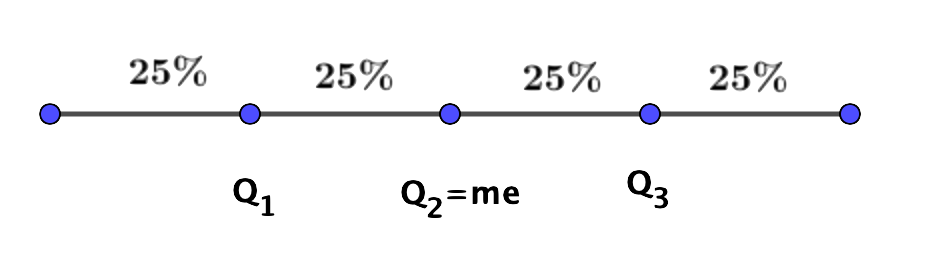
\includegraphics[width=.7\textwidth]{imagenes/imagenes01/T01IM12.png}
	\end{figure}
\end{definition}

Evidentemente, $\ Q_2=me$.

\vspace{5mm}%**********************	
\begin{theorem}
	. Para datos agrupados, como en la mediana, 
	
	$$\boxed{\ \boldsymbol{Q_1=L_k+\dfrac{\dfrac{N}{4}-N_{k-1}}{n_k}\cdot c_k} \ }$$
	
	$$\boxed{\ \boldsymbol{Q_2=L_k+\dfrac{\dfrac{N}{2}-N_{k-1}}{n_k}\cdot c_k \ = \ me}  \ } $$
	
	$$ \boxed{\ \boldsymbol{Q_3=L_k+\dfrac{\dfrac{3N}{4}-N_{k-1}}{n_k}\cdot c_k} \ }$$
\end{theorem}

\vspace{5mm}%**********************
\begin{definition}
	. Los \textbf{Deciles} son 9 valores, $D_1,\ D_2, \ D_3,  \cdots , D_9$, que dividen a la población en $10$ partes iguales. Entre dos deciles consecutivos se encuentra el $10\%$ de la población.	
	
	\begin{figure}[H]
			\centering
			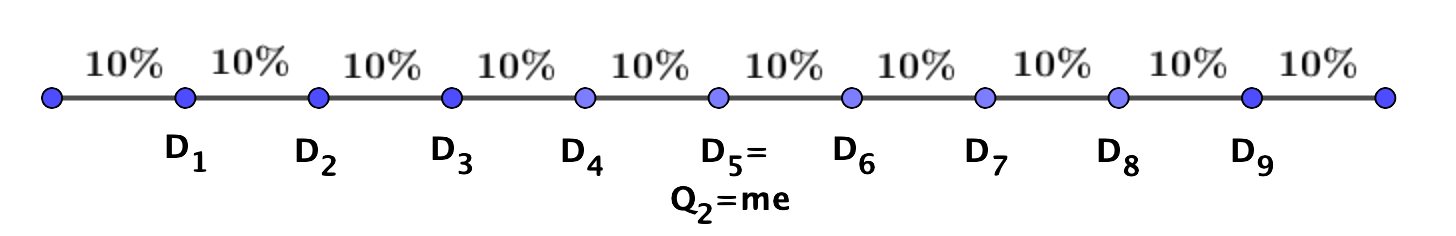
\includegraphics[width=.9\textwidth]{imagenes/imagenes01/T01IM13.png}
	\end{figure}
\end{definition}

Evidentemente, $\ D_5=Q_2=me$.

\vspace{5mm}%**********************
\begin{theorem}
	. Para datos agrupados, como en la mediana, 
	
	$$\boxed{\ \boldsymbol{D_m=L_k+\dfrac{\dfrac{mN}{10}-N_{k-1}}{n_k}\cdot c_k} \ }\; \qquad m=1,2,3,\cdots , 9$$
	
\end{theorem}
	
\vspace{5mm}%**********************
\begin{definition}
	. Los \textbf{Percentiles} son 99 valores, $P_1,\ P_2, \ P_3,  \cdots , P_{67}, \cdots, P_{99}$, que dividen a la población en $100$ partes iguales. Entre dos percentiles consecutivos se encuentra el $1\%$ de la población.	
\end{definition}

\vspace{5mm}%**********************
\begin{theorem}
	. Para datos agrupados, como en la mediana, 
	
	$$\boxed{\ \boldsymbol{P_m=L_k+\dfrac{\dfrac{mN}{100}-N_{k-1}}{n_k}\cdot c_k} \ }\; \qquad m=1,2,3,\cdots , 99$$
\end{theorem}

Evidentemente, $P_{50}=D_5=Q_2=me;\ P_{25}=Q_1;\ P_{75}=Q_3$

Como ocurría con la mediana, se puede obtener un \underline{valor aproximado de los cuartiles} a través del histograma de frecuencias relativas acumuladas \textcolor{gris}{(ahora, la línea poligonal no une los puntos medios de cada clase sino los extremos superiores de cada clase y el extremo inferior de la primera clase)}.

	\begin{figure}[H]
			\centering
			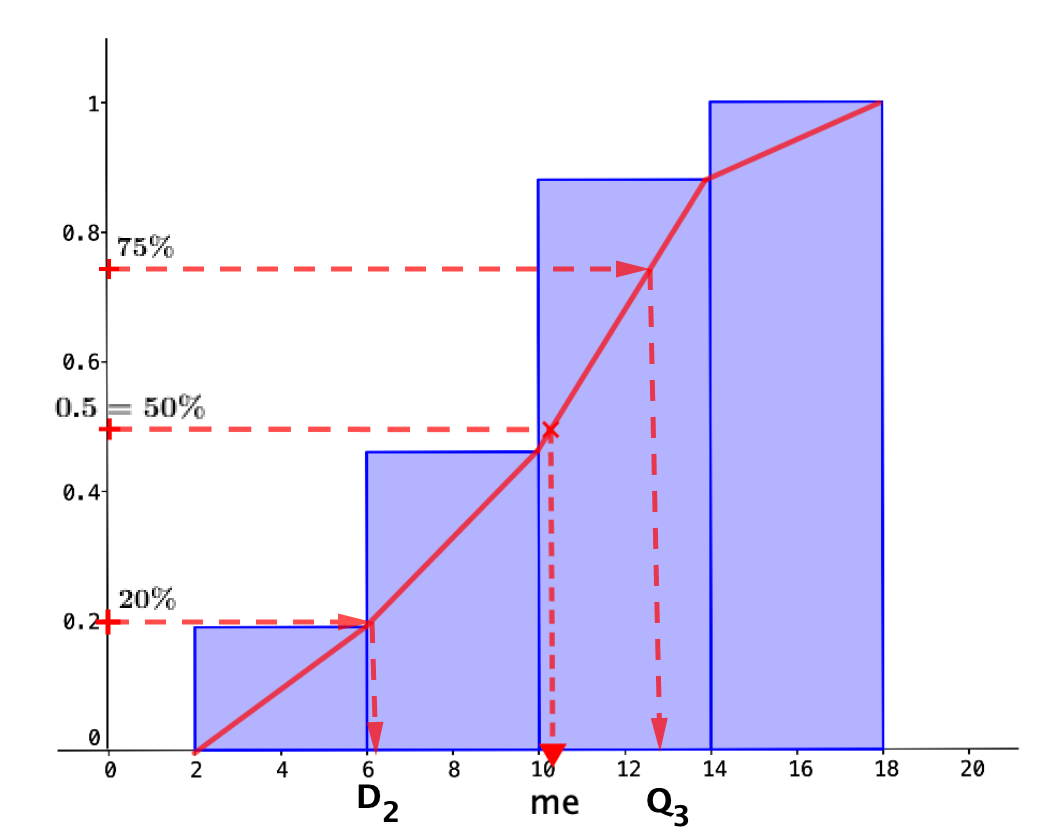
\includegraphics[width=.75\textwidth]{imagenes/imagenes01/T01IM09_copia.png}
	\end{figure}

\vspace{5mm}%**********************
\begin{example}
	. Los datos siguientes corresponden a los tiempos de reacción de una muestra de $33$ sujetos, medidos en centésimas de segundo, son:
55, 51, 60, 56, 64, 56, 63, 63, 61, 57, 62, 50, 49, 70, 72, 54, 48, 53, 58, 66, 68, 45, 74, 65, 58, 61, 62, 59, 64, 57, 63, 52, 67.

\vspace{2mm} Calcúlese  la moda, la mediana, el primer y el tercer cuartil, directamente a partir de los datos.	Calcúlese, así mismo, los deciles segundo y quito y los percentiles 33 y 58.

\vspace{4mm}  Construimos un diagrama de tallos y hojas, que nos permitirá contar los datos y tenerlos ordenados (una forma alternativa a las tablas de frecuencias absolutas).

\begin{table}[H]
\centering
\begin{tabular}{c|ccccccccccccccc}
Tallos & \multicolumn{15}{c|}{Hojas} \\ \hline
4 & 5 & 8 & 9 &  &  &  &  &  &  &  &  &  &  &  &  \\
5 & 0 & 1 & 2 & 3 & 4 & 5 & 6 & 6 & 7 & 7 & 8 & 8 & 9 &  &  \\
6 & 0 & 1 & 1 & 2 & 2 & 3 & 3 & 3 & 3 & 4 & 4 & 5 & 6 & 7 & 8 \\
7 & 0 & 2 & 4 &  &  &  &  &  &  &  &  &  &  &  & 
\end{tabular}
\end{table}

\begin{multicols}{2}
$mo=63$; 

$ (33+1)/2 = 17 \to me=x_{17}=60$

$\frac 1 4 33= 8.25 \to Q_1=x_9=55$

$\frac 3 4 33=24.75 \to Q_3=x_{25}=34$

$D_2=\frac 2 {10} 33 = 6.6 \to D_2=x_{7}=53$

$D_5=me=60$

$\frac {33}{100}33=10.89 \to  P_{33}=x_{11}=66$

$\frac {58}{100}33=19.14 \to  P_{58}=x_{20}=68$
\end{multicols}

\end{example}


\vspace{5mm}%**********************
\begin{example}

	 Con los datos del ejemplo anterior, construya una tabla estadística  agrupados los datos en 5 intervalos de igual amplitud, calcule la mediana, el primer y el tercer cuartil.	Calcúlese, así mismo, los deciles segundo y quito y los percentiles 33 y 58.

\vspace{4mm} \begin{small}Para llegar a la anterior tabla se ha calculado en primer lugar el rango de la distribución que es el mayor valor 74 menos el menor 45, lo que nos da 29. Como 29 no es divisible entre 5 redondeamos hasta el valor más próximo por exceso que es 30, dividiendo este rango entre el número de intervalos que deseamos, cinco, obtenemos la amplitud que deben tener los intervalos, seis. A partir del primer valor, 45 se han calculado los restantes extremos sumando 6, sucesivas veces. Posteriormente se ha contado el número de observaciones comprendidas dentro de cada intervalo, recuérdese que los intervalos se toman abiertos a la derecha, y de esta forma se han obtenido las frecuencias que aparecen en la tabla, en la que se han añadido las frecuencias acumuladas.\end{small}

\begin{multicols}{2}
\begin{table}[H]
\begin{tabular}{crr}
\textbf{Clases}                  & \multicolumn{1}{|c|}{\textbf{$n_i$}} & \multicolumn{1}{c}{\textbf{$N_i$}} \\ \hline
\multicolumn{1}{c|}{{[}45,51{[}} & \multicolumn{1}{r|}{4}             & 4                                  \\
\multicolumn{1}{c|}{{[}51,57{[}} & \multicolumn{1}{r|}{6}             & 10                                 \\
\multicolumn{1}{c|}{{[}57,63{[}} & \multicolumn{1}{r|}{11}            & 21                                 \\
\multicolumn{1}{c|}{{[}63,69{[}} & \multicolumn{1}{r|}{9}             & 30                                 \\
\multicolumn{1}{c|}{{[}69,75{[}} & \multicolumn{1}{r|}{3}             & 33                                
\end{tabular}
\end{table}
--- Intervalo modal: $\ [57,63[$

--- $mo=$ \begin{scriptsize}
 $57+\dfrac{11-6}{(11-6)+(11-9)}6$	
\end{scriptsize} $=61.3$

--- \begin{scriptsize}
$33/2=16.5 \to $ \end{scriptsize} Int. mediano: $\ [57,63[$


--- $me=$\begin{scriptsize}
 $57+\dfrac{16.5-10}{11}6$	
\end{scriptsize}$=60.5$
\end{multicols}
--- $25\% 33=8,25 \to [51,57 [ \to Q_1=57+\dfrac{8.25-4}{6}\ 6=55.3$

--- $75\% 33=24,75 \to [63,69 [ \to Q_3=63+\dfrac{24.75-21}{9}\ 6=65.5$

--- $20\% 33=6,6 \to [51,57 [ \to D_2=51+\dfrac{6.6-4}{6}\ 6=53.6$

--- $D_5=me=60.5$

--- $33\% 33=10.9 \to [57,63 [ \to P_{33}=57+\dfrac{10.9-10}{11}\ 6=57.1$

--- $58\% 33=19,1 \to [57,63 [ \to P_{58}=57+\dfrac{19.1-10}{11}\ 6=62.0$

\vspace{4mm} De manera aproximada, aparece en la figura siguiente.
\end{example}

\begin{figure}[]
			\centering
			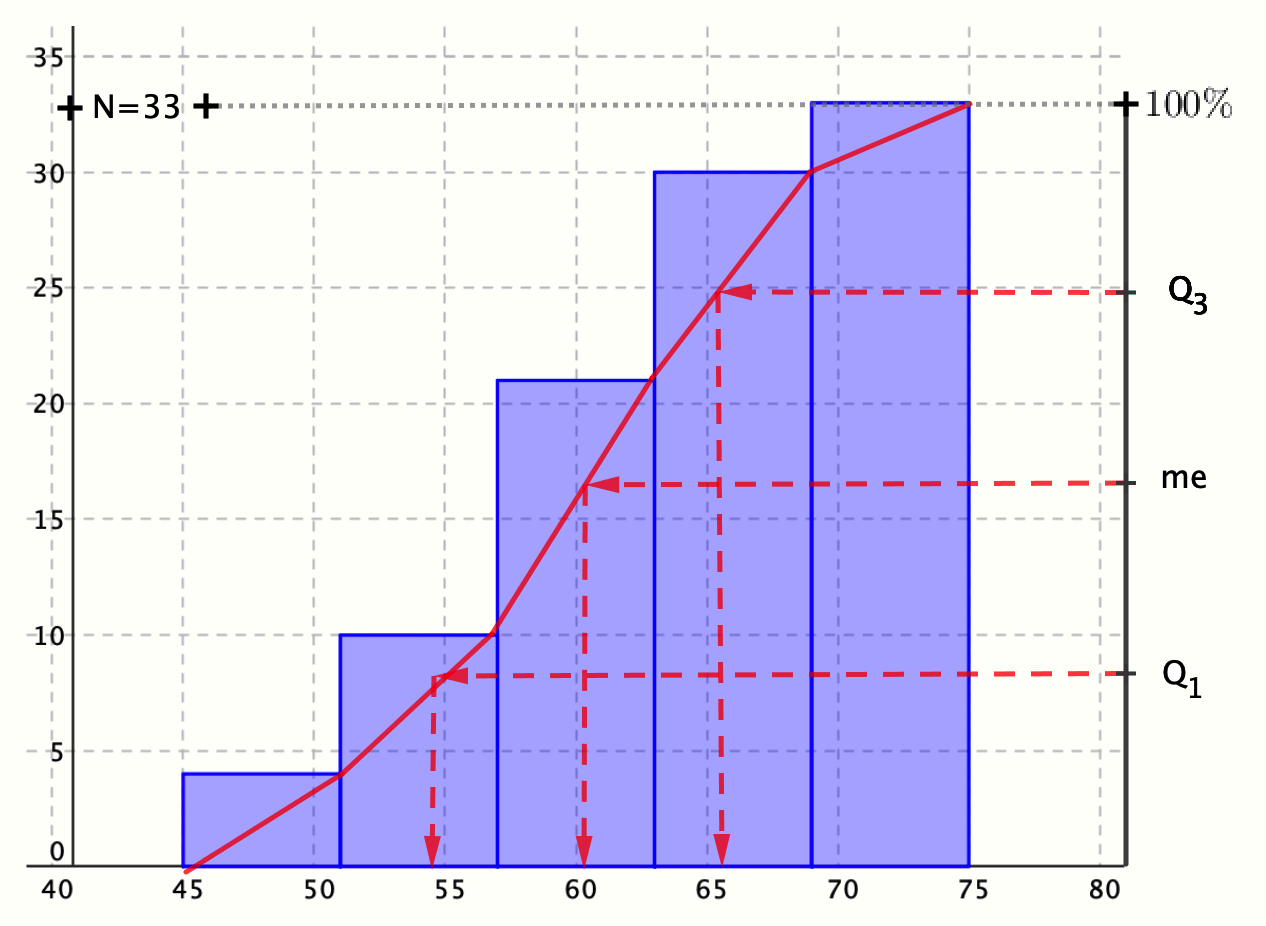
\includegraphics[width=.75\textwidth]{imagenes/imagenes01/T01IM14.png}
			\caption*{Histograma de frecuencias relativas acumuladas. del ejemplo 1.15}
	\end{figure}

\vspace{15mm}%**********************
\begin{ejemplo}
\begin{ejre}
Para la siguiente distribución estadística, responder a las  preguntas que se formulan.

\vspace{5mm}%*********************
\begin{multicols}{2}
\begin{table}[H]
\begin{tabular}{c|r|r}
\textbf{$x_i$} & \multicolumn{1}{c|}{\textbf{$n_i$}} & \multicolumn{1}{c}{\textbf{$N_i$}} \\ \hline
{[}0,10{[}     & 8                                   & 8                                  \\
{[}10,20{[}    & 22                                  & 30                                 \\
{[}20,30{[}    & 32                                  & 62                                 \\
{[}30,40{[}    & 44                                  & 106                                \\
{[}40,50{[}    & 28                                  & 134                                \\
{[}50.60{[}    & 20                                  & 154                                \\
{[}60,70{[}    & 6                                   & 160                               
\end{tabular}
\end{table}

%\rule{5cm}{0.3pt}

\begin{small}
a) ?`Entre qué valores se encuentra el 50\% central de los individuos?

b) Calcule el percentil 27.

c) ?`A partir de que puntuación se encuentra el 12\% de los sujetos con puntuación más alta?

d) Si descontamos el 15\% de los individuos con menor puntuación y al 15\% de los de mayor puntuación, ?`en qué intervalo de puntuación se encuentran los restantes?
\end{small}
\end{multicols}

--- a) El 50\% de la población estará entre el $Q_1$ (que deja tras sí al 25\% de la población) y el $Q_3$ (que deja tras sí al 75\%, luego tiene por delante al 25\% de la población).

$160/4=40 \to [20,30[ \to Q_1=20+\dfrac{40-30}{32}\ 10=23.13$

 $3\cdot 16074=120\to [40,50[ \to Q_3=40+\dfrac{120-106}{28}\ 10=45,00$
 
 El 50\% de la población está en $\ [23.13,45.00[$
 
 --- b) $27\%160=43.2 \to [20,30[ \to P_{27}=20+\dfrac{43.2-30}{32}\ 10= 20.13$

--- c) El valor que deja por encima el 12\% de los sujetos con mayor puntuación es el mismo que deja por debajo el 88\% con menor puntuación, por tanto debemos calcular el percentil 88.

$88\%160=140.8 \to [50,60[ \to P_{88}=50+\dfrac{140.8-134}{20} \ 10 =53.40$

--- d) Se trata de calcular el percentil 15 y el percentil 85. El 15% del tamaño de la muestra es 24. El 85% del tamaño es 136 y por tanto:

$15\% 160= 24 \to [10,20[ \to P_{15}=10+\dfrac{24-8}{22}\ 10=17.27$

$85\% 160=136 \to [50,60[ \to P_{85}=500+\dfrac{136-134}{20}\ 10=51.00$

El intervalo solicitado es $\ [17,27,51.00[$, es el llamado \textbf{intervalo intercuartílico.}

\end{ejre}
\end{ejemplo}

\vspace{5mm}%**********************	
\begin{myalertblock}{Diagrama de cajas y bigotes}
	Los \textbf{diagramas de cajas y bigotes} (\emph{boxplots} o \emph{box and whiskers}) son una representación visual que describe varias características de la serie estadística al mismo tiempo (dispersión, simetría).
	
	\vspace{2mm} Para su construcción hay que calcular $Q_1, me, Q_3$ que se representarán sobre un rectángulo, \textbf{caja}, y los valores $x_{max},\ x_{min}$ que se representarán por segmentos, \textbf{bigotes}.
	
	\vspace{2mm} Veamos un ejemplo. Para la serie: 36, 25, 37, 24, 39, 20, 36, 45, 31, 31, 39, 24, 29, 23, 41, 40, 33, 24, 34, 40; obtenemos:
	
	\vspace{2mm} $Q_1=25;\ me=33.5;\  Q_3=39;\ x_{min}=20;\ x_{max}=45$

	\begin{figure}[H]
			\centering
			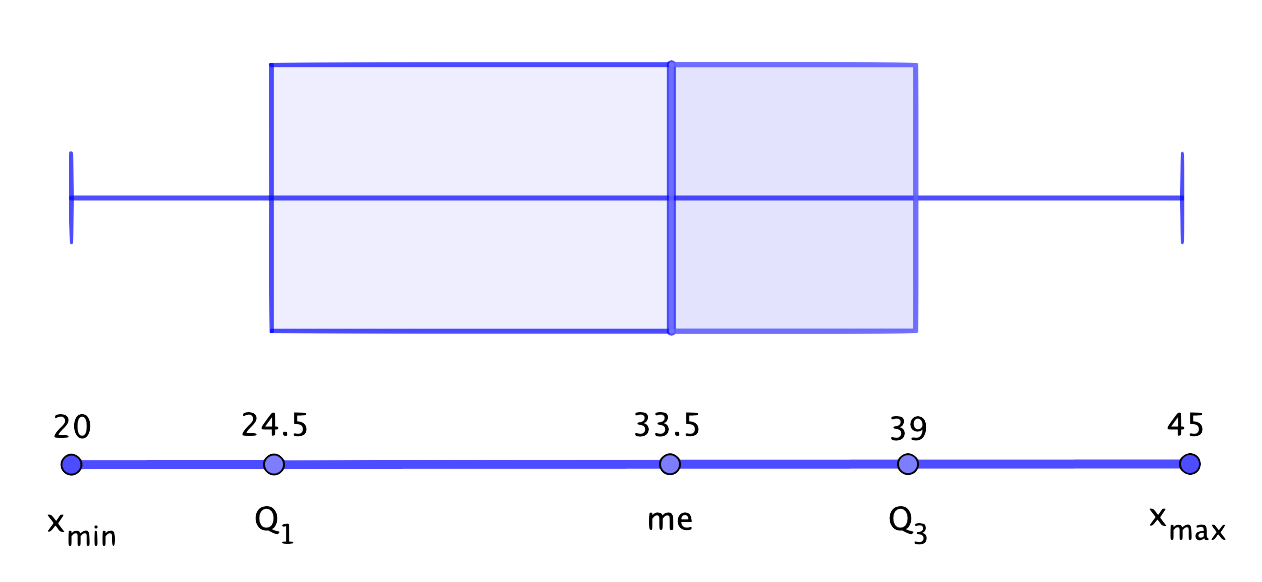
\includegraphics[width=.65\textwidth]{imagenes/imagenes01/T01IM15.png}
	\end{figure}
	
	\vspace{2mm} Algunas de las informaciones que se desprenden de la observación de este gráfico son:
	
	\vspace{1mm} --- La parte izquierda de la caja es mayor que la derecha. Los más jóvenes, entre el 25\% y el 50\% de la población tienen edades más dispersas que los mayores de entre el 50\% y 75\% de la población.
	
	\vspace{1mm} --- El bigote de la izquierda es menor que el de la derecha. El 25\% de los más jóvenes están más concentrados qu el 25\% de los más mayores.
	
	\vspace{1mm} --- El \emph{rango intercuartílico}, $Q_3-Q_1=$14.5. El 50\% de la población tiene edades que se diferencian en menos de 14.5 años.
	
	\vspace{1mm} --- La $me=$33,5. El 50\% de la población son. menores de 33.5 años y el otro 50\% tiene edades mayores a 33.5 años.
	
	\vspace{2mm} Además, los diagramas de cajas y bigotes son muy útiles para comparar dos distribuciones: supongamos otra distribución por edades de 20 personas cuyas edades son, 35, 38, 32, 28, 30, 29, 27, 19, 48, 40, 39, 24, 24, 34, 26, 41, 29, 48, 28, 22.
	
	\vspace{2mm} Los valores que ahora se obtienen son: $Q_1=26.5$, $Q_3=38.5$, $me=29.5$, $x_{min}=19$, $x_{max}=48$. Comparando ambos diagramas:
	
	\vspace{2mm} Ahora, puede obtenerse información respecto a las dos distribuciones.
	 
	 \begin{figure}[H]
			\centering
			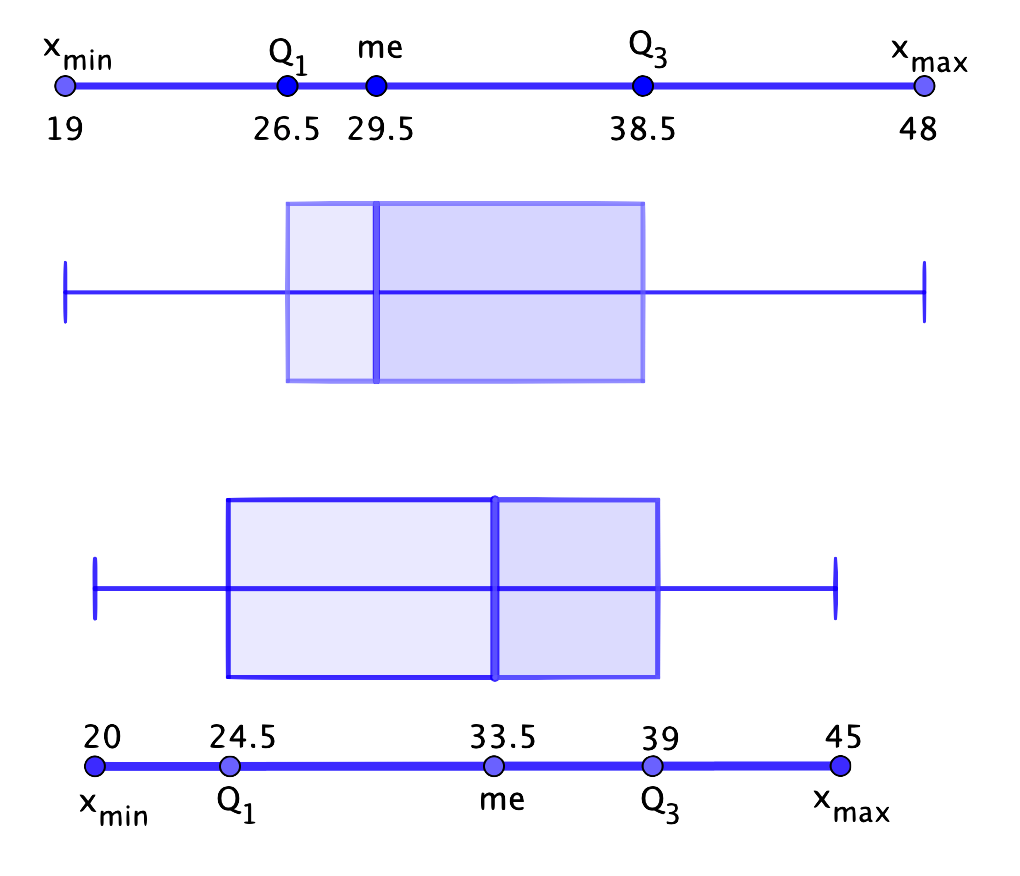
\includegraphics[width=.65\textwidth]{imagenes/imagenes01/T01IM16.png}
	\end{figure}
	
	\vspace{1mm} --- Rápidamente se observa que la segunda distribución, representada por el diagrama de cajas y bigotes de arriba, está más concentrada en edades que la representada abajo que es más dispersa (distribución primera). 
	
	\vspace{1mm} --- En la distribución de abajo (primera distribución), los datos eran más dispersos entre el 25\% y 50\% de la población. En la distribución de arriba (segunda distribución), ocurre al revés, los datos son más dispersos entre el 50\% y el 75\% de la población.
	
	\vspace{1mm} --- En cuanto a los bigotes, para la distribución de arriba se observa que son más largos, sobre todo la rama derecha lo cual indica que el 25\% de la población de esta distribución es más dispersa que la otra.
	
	\vspace{2mm} También se suelen representar en los diagramas de cajas y bigotes los llamados \emph{Valores atípicos} son aquellos que muestran una gran distancia a la mediana del resto de puntuaciones en la variable, es decir, o son demasiado bajas o son demasiado altas.  Numéricamente, se consideran \emph{valores atípicos} aquellos que sean menores que $Lim_{inf}=Q_1-1.5\cdot (Q_3-Q_1)$ o mayores que $Lim_{sup}=Q_3+1.5\cdot (Q_3-Q_1)$, de otro modo, los que están fuera del intervalo $(Lin_{inf},Lim_{sup})$, es decir, los que se separan de los cuartiles más de 1.5 veces el rango intercuartílico ($Q_3-Q_1$), 
	
	\vspace{2mm} 
	
\end{myalertblock}

\vspace{5mm}%**********************
\begin{myalertblock}{Relación entre media, mediana y moda.}

\begin{itemize}
\item si $\bar{x}=me=mo$, la distribución es \emph{simétrica}.
\item si $me>\bar{x}$, la distribución es \emph{asimétrica}, con cola a la derecha (\emph{sesgada a la derecha}).
\item si $me<\bar{x}$, la distribución es \emph{asimétrica}, con cola a la izquierda (\emph{sesgada a la izquierda}).
\end{itemize}

	 \begin{figure}[H]
			\centering
			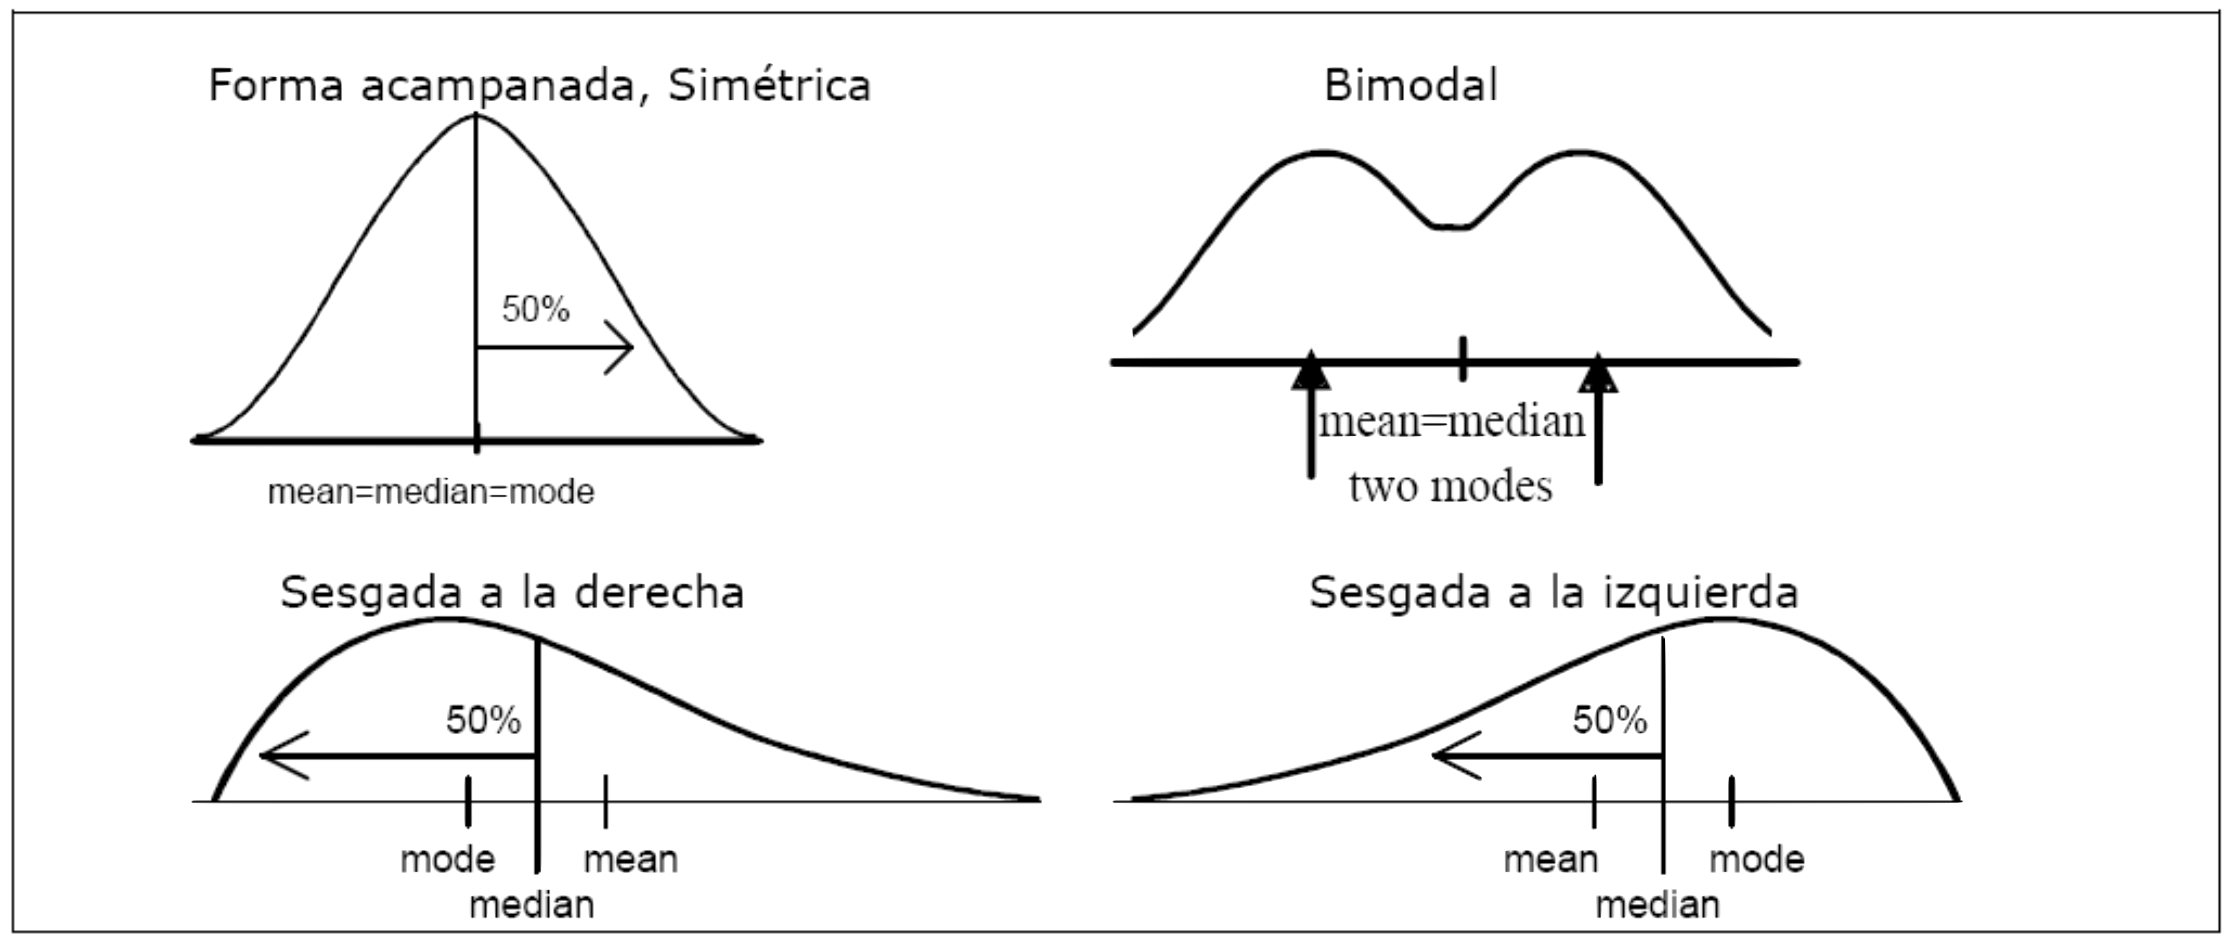
\includegraphics[width=1\textwidth]{imagenes/imagenes01/T01IM17.png}
	\end{figure}
	
\end{myalertblock}


\subsection{Parámetros de dispersión}
	
	Las medidas de dispersión, o de variabilidad (o propagación), expresan cómo se distribuyen los datos en torno a alguna de las medidas de centralización definidas antes (nos informan sobre cuánto se alejan del centro los valores de la distribución) y son un complemento a estas últimas para describir más fielmente un conjunto de datos.
	
	Cuanto más pequeña sea la medida de dispersión, mayor grado de agrupamiento de los datos respecto a la medida de centralización considerada (generalmente la media) y más representativa será este parámetro de centralización para definir el comportamiento de la distribución.
	
	Son de medidas de dispersión estadística son la varianza, la desviación típica, desviación media, el rango y rango intercuartílico. 
	
\vspace{5mm}%**********************
\begin{definition}
	. Se define el \textbf{recorrido} o 	\textbf{rango} de la distribución como la diferencia entre los valores mayor y menor de la variable.
	
	$$\boldsymbol{R\ = \ x_{max}-x_{min}}$$
	
	 Se define	el \textbf{rango intercuartílico} como la diferencia entre el tercer y el primer cuartil. Proporciona la longitud del intervalo en el que se encuentra el 50\% de las observaciones centrales.
	 
	 $$\boldsymbol{R_I\ =\ Q_3-Q_1}$$
\end{definition}

\vspace{5mm}%**********************
\begin{definition}
	. Se llama \textbf{desviación media} respecto al valor medio a la media de los valores absolutos de las diferencias de cada valor respecto del valor medio:
	
	$$\boldsymbol{ DM \ = \ \dfrac { \displaystyle \sum_{i=1}^n |x_i-\bar x|\cdot n_i }{N}  }$$	
\end{definition}

\vspace{5mm}%**********************
\begin{definition}
	. \textbf{Varianza, $\boldsymbol{s^2}$ y desviación típica, $\boldsymbol{s}$}. La desviación típica es la medida de dispersión más utilizada, representa la dispersión de los datos de la distribución respecto del valor medio y se expresa en sus mismas unidades.	
	
	$$\boldsymbol{ s^2=\dfrac {\displaystyle \sum_{i=1}^n (x_i-\bar x)^2\cdot n_i}{N}\ ; \qquad  \qquad \qquad s\ = \ \sqrt{s^2}}$$
\end{definition}

\vspace{5mm}%**********************	
\begin{theorem}
	. \begin{itemize}
 \item La varianza será siempre un valor positivo o cero (si todos los datos son iguales).

 \item Si a todos los valores de la variable se les suma un número la varianza no varía.

 $\{x_i\}\to s^2 \Rightarrow  \{x_i+d\}\to s^2$

\item Si todos los valores de la variable se multiplican por un número la varianza queda multiplicada por el cuadrado de dicho número.

 $\{x_i\}\to s^2 \Rightarrow \{ax_i\}\to a^2s^2$

\item Si tenemos varias distribuciones con la misma media y conocemos sus respectivas varianzas se puede calcular la varianza total.	

Para $n$ muestras de varianza $s_i^2$ formadas cada una de ellas por $k_i$ datos, la varianza total de la nueva distribución de $k_1+\cdots +k_n$ datos es:  $\ s^2=\dfrac {k_1 s_1^2+\cdots +k_n s_n^2}{k_1+\cdots +k_n}$

\item  Las siguientes definiciones de la varianza son equivalentes:

$$\subrayado{ \ \boxed{\ \boldsymbol{ s^2=\dfrac {\displaystyle \sum_{i=1}^n (x_i-\bar x)^2\cdot n_i}{N} \quad \leftrightarrow \quad s^2=\dfrac {\displaystyle \sum_{i=1}^n (x_i)^2\cdot n_i}{N}-{\bar {x}}^2  }\ } \ }$$
 \end{itemize}
	
\end{theorem}
	
\begin{proof}.

$s^2=\dfrac {\displaystyle \sum_{i=1}^n (x_i-\bar x)^2\cdot n_i}{N} =\dfrac {\displaystyle \sum_{i=1}^n (x_i^2-2x_i\bar x+{\bar x}^2)\cdot n_i}{N}=$

$=\dfrac {\displaystyle \sum_{i=1}^n x_i^2 \cdot n_i}{N}-2\bar x \dfrac{\displaystyle \sum_{i=1}^n x_i\cdot n_i}{N}+{\bar x}^2=
\dfrac {\displaystyle \sum_{i=1}^n x_i^2 \cdot n_i}{N} -2{\bar x}^2+{\bar x}^2=\dfrac {\displaystyle \sum_{i=1}^n x_i^2 \cdot n_i}{N}-{\bar x}^2$
\end{proof}

\textbf{Observaciones respecto a la varianza:}

\begin{enumerate}[1. ]
\item La varianza, al igual que la media, es un índice muy sensible a las puntuaciones extremas.
 
\item En los casos que no se pueda hallar la media tampoco será posible hallar la varianza.
\end{enumerate}

\vspace{5mm}%**********************
\begin{definition}
. El \textbf{coeficiente de variación}, también denominado como \emph{coeficiente de variación de Pearson}, es una medida estadística adimensional que nos informa acerca de la \underline{dispersión relativa} de varias distribuciones.	

\vspace{2mm} Si los valores sean positivos y su media dé, por tanto, un valor positivo, \emph{a mayor valor del coeficiente de variación mayor heterogeneidad (dispersión) de los valores de la variable}; y a \\emph{menor C.V., mayor homogeneidad (menor dispersión) en los valores de la variable}. Por ejemplo, si el C.V es menor o igual al 80\%, significa que la media aritmética es representativa del conjunto de datos, por ende el conjunto de datos es \emph{``Homogéneo''}. Por el contrario, si el C.V supera al 80\%, el promedio no será representativo del conjunto de datos (por lo que resultará \emph{``Heterogéneo''}). 

\vspace{2mm} El coeficiente de variación se define como la razón entre la desviación típica y el valor medio:

$$\boldsymbol{ CV \ = \ 	\dfrac {s}{\bar x}} \qquad \qquad\textcolor{gris}{(\bar x \neq 0})$$
\end{definition}

\vspace{5mm}%**********************
\begin{ejemplo}
\begin{ejre} Calcula las medidas de dispersión para la siguiente distribución estadística.
			
\begin{table}[H]
\centering
\begin{tabular}{r|r|r|r|r|r|r|}
\hline
\multicolumn{1}{|c|}{\textbf{$x_i$}} & \multicolumn{1}{c|}{\textbf{$n_i$}} & \multicolumn{1}{c|}{\textbf{$N_i$}} & \multicolumn{1}{c|}{\textbf{$x_i\cdot n_i$}} & \multicolumn{1}{c|}{\textbf{$x_i^2 \cdot n_i$}} & \multicolumn{1}{c|}{\textbf{$|x_i- \bar x|$}} & \multicolumn{1}{c|}{\textbf{$|x_i-\bar x| \cdot n_i$}} \\ \hline
\multicolumn{1}{|r|}{1} & 7 & 7 & 7 & 7 & 1.6 & 11.2 \\
\multicolumn{1}{|r|}{2} & 14 & 21 & 18 & 56 & 0.6 & 8.4 \\
\multicolumn{1}{|r|}{3} & 9 & 30 & 27 & 81 & 0.4 & 3.6 \\
\multicolumn{1}{|r|}{4} & 8 & 38 & 32 & 128 & 1.4 & 11.2 \\
\multicolumn{1}{|r|}{5} & 2 & 40 & 10 & 50 & 2.4 & 4.8 \\ \hline
 & \multicolumn{1}{c|}{N=40} &  & \multicolumn{1}{c|}{Total: 104} & \multicolumn{1}{c|}{Total: 322} &  & \multicolumn{1}{c|}{Total: 39.2} \\ \cline{2-2} \cline{4-5} \cline{7-7} 
\end{tabular}
\end{table}



--- Rango: $\ R=x_{max}-x_{min}=5.1=4$



--- Rango: $\ R=x_{max}-x_{min}=5.1=4$

$25\% (40)=10 \to Q_1=2; \quad 75\%(40)=30 \to Q_3=\dfrac{3+4}{5}=3.5$

--- Recorrido intercuartílico: $\ R_I=Q_3-Q_1=3.5-2=1.5$

$\bar x=\dfrac {\displaystyle \sum x_i \cdot n_i}{N}=\dfrac{104}{40}=2.6$

--- Desviación media: $\ DM  =  \dfrac { \displaystyle \sum_{i=1}^n |x_i-\bar x|\cdot n_i }{N}=\dfrac{39.2}{40}=0.98$ 

--- Varianza: $\ s^2 =\dfrac {\displaystyle \sum_{i=1}^n (x_i)^2\cdot n_i}{N}-{\bar {x}}^2=\dfrac{332}{40}-2.6^2=1.29$

--- Desviación típica: $\ s=\sqrt{s^2}=\sqrt{1.29}=1.14$

--- Coeficiente de variación (de Perason): $CV=\dfrac{s}{\bar x}=\dfrac{1.14}{2.6}=0.44=44 \%$

Si los datos estuviesen agrupados en intervalos, procederíamos de la misma forma, considerando como $x_i$ las marcas de clase.

\end{ejre}
\end{ejemplo}	
	
	
\vspace{5mm}%**********************	
\begin{ejemplo}
\begin{ejre} El cóndor de los Andes tiene una envergadura media (alas extendidas) de $285 \ \mathrm{cm}$ con una desviación estándar de $30 \ \mathrm{cm}$, mientras que una especie de murciélago tiene una envergadura media de $10 \ \mathrm{cm}$ y su población presenta una desviación estándar de $3 \ \mathrm{cm}$.

?`Cuál de las dos poblaciones presenta una mayor dispersión en lo que se refiere a su envergadura?	

\vspace{4mm} Condor: $\ CV=\dfrac{s}{\bar x}=\dfrac{30}{285}=0.11=11\%$

Murciélago: $\ CV=\dfrac{s}{\bar x}=\dfrac{3}{10}=0.30=30\%$

Aunque la desviación típica de la envergadura del cóndor de los Andes es muy superior a la de esa especie de murciélago, su dispersión es menor.
\end{ejre}
\end{ejemplo}

\subsection{Parámetros de forma}

Se usan para describir numéricamente la forma de la distribución. Miden la \emph{simetría} o sesgo y la \emph{curtosis} o apuntamiento y son parámetros adimensionales.

\vspace{5mm}%**********************
\begin{definition}
	. \textbf{Índices de asimetría}:
	
	
	\vspace{2mm} --- Coeficiente de asimetría de Fisher: $\ As=\dfrac{\displaystyle \sum_{i=1}^n (x_i-\bar x)^3 \ n_i}{N s^3}$
	
	\vspace{4mm} Interpretación de los coeficientes: Si $As>0$ la distribución presenta una asimetría positiva, si $As<0$ la asimetría es negativa y si $As\simeq 0$ la distribución es simétrica.
	
	\begin{figure}[H]
			\centering
			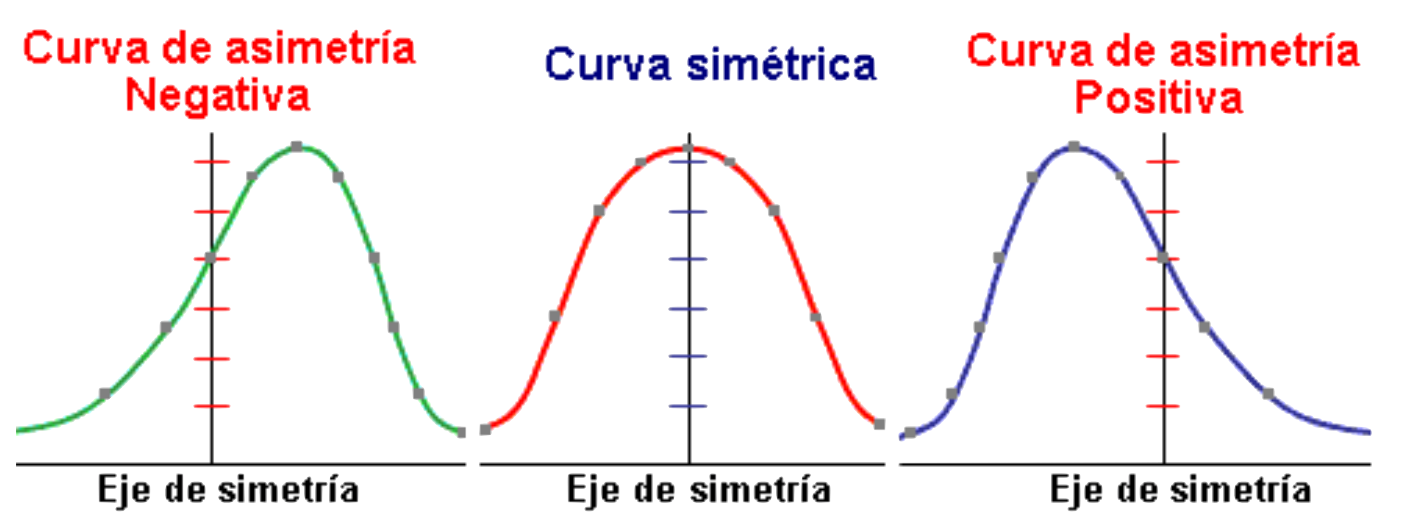
\includegraphics[width=.75\textwidth]{imagenes/imagenes01/T01IM18.png}
	\end{figure}
\end{definition}

\vspace{5mm}%**********************	
\begin{definition}
	. El \textbf{apuntamiento o curtosis} proviene de una comparación de la distribución con la \emph{distribución normal o campana de Gauss} por lo que solo tendrá sentido para las distribuciones que se asemejen a la curva normal (unimodales y prácticamente simétricas). Para su medida se usa el
	
	\vspace{2mm} --- Coeficiente de apuntamiento de Fisher: $\ K=\dfrac{\displaystyle \sum_{i=1}^n (x_i-\bar x)^4 \ n_i}{Ns^4}-3$
	
	\vspace{4mm} Si $K<0$ tenemos una distribución \emph{platicúrtica}, en las colas de la distribución hay más casos que en la curva normal. Si $K>0$ la distribución es \emph{leptocúrtica}, ocurre lo contrario que en el caso anterior. Para $K\simeq 0$ la distribución es como la normal, se llama \emph{mesocúrtica}.
	
	\begin{figure}[H]
			\centering
			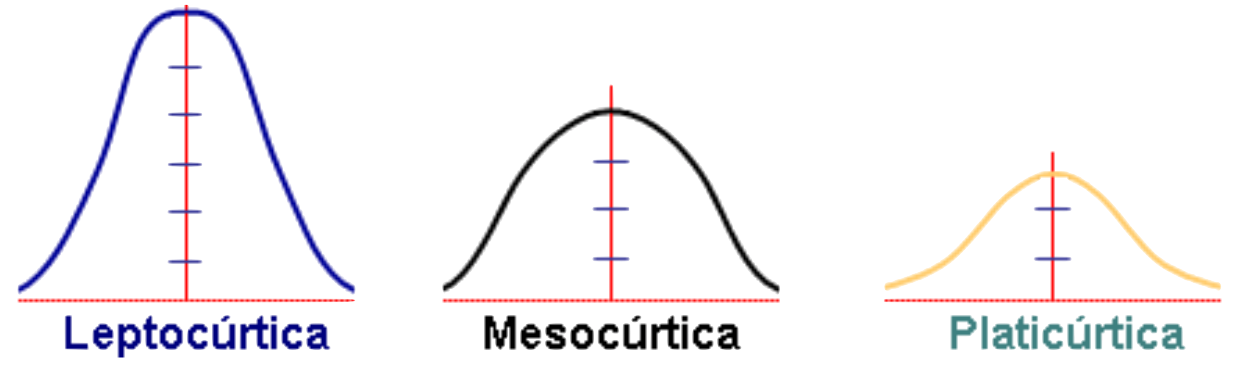
\includegraphics[width=.75\textwidth]{imagenes/imagenes01/T01IM19.png}
	\end{figure}
	
	\end{definition}

\vspace{5mm}%**********************
\begin{example}
	. Calcula el coeficiente de asimetría y la curtosis para la siguiente distribución.
	
	\begin{figure}[H]
			\centering
			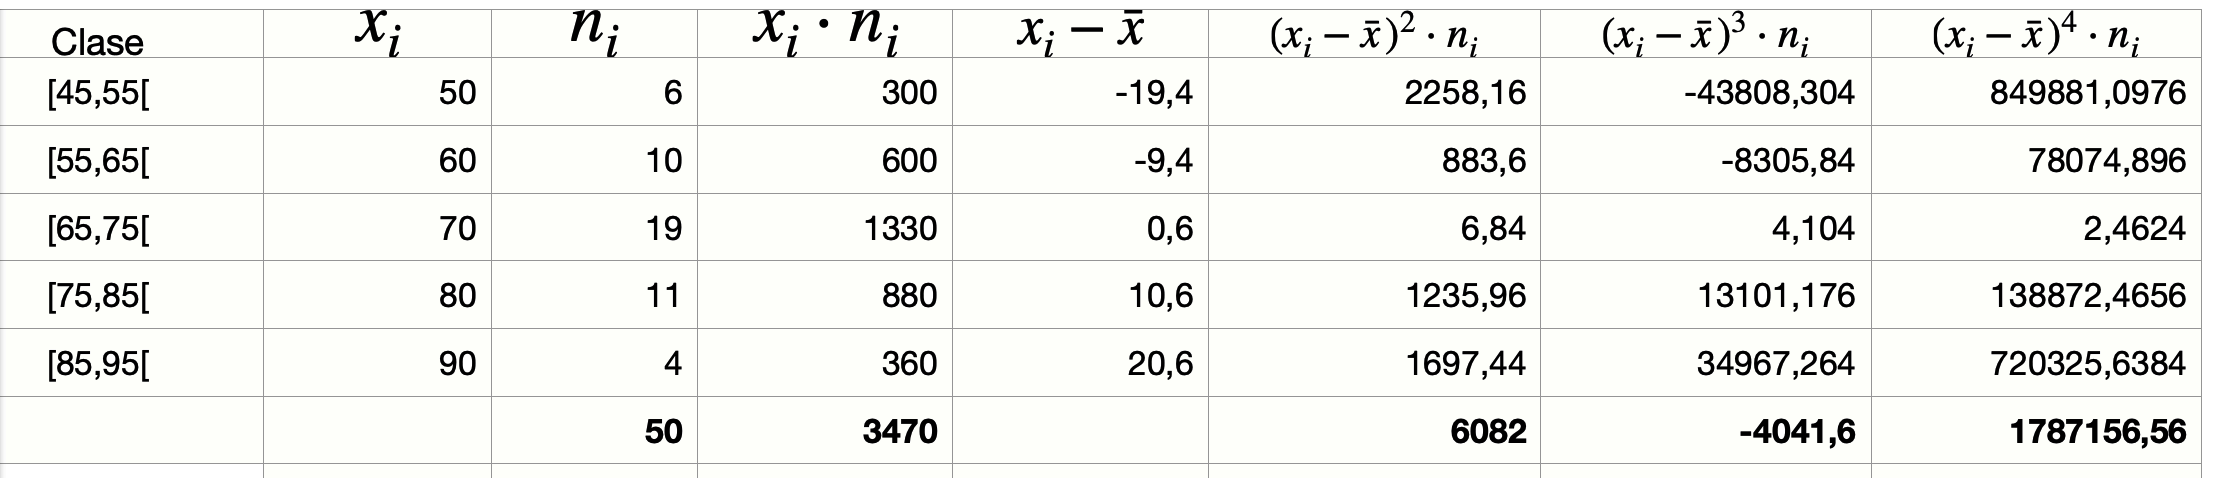
\includegraphics[width=1\textwidth]{imagenes/imagenes01/T01IM20.png}
	\end{figure}
	
	
	$\bar x=\dfrac{3470}{50}=69.4$ $;\qquad$ $\sigma=\sqrt{\dfrac{6082}{50}}=11.0$
	
	$As=\dfrac{-4041.6}{50\cdot 11.0^3}=-0.06\simeq -0.1$
	
	$K=\dfrac{1787156.56}{50\cdot 11.0^4}-3=2.4-3=-0.6$	
	

\vspace{2mm}La distribución es prácticamente simétrica (ligero sesgo o asimetría negativa o hacia la izquierda) y platicúrtica.
		
\end{example}

\subsection{Interpretación conjunta de la media y la desviación típica}
\label{mediaydesviacion}
	
\begin{myalertblock}{$\boldsymbol{ \bar x \ \text{ y } \ \sigma. }$}
	Cuando la distribución en estudio es \emph{``normal''} (de momento no sabemos que significa esto de 'normal' -- lo veremos en distribuciones de probabilidad -- pero supongamos que son aquellas que no presentan valores `extraños') resulta que datos de la distribución que se alejen una desviación típica del valor medio hay alrededor de los 2/3 del total de datos, es decir, individuos con $x_i\in[\bar x -\sigma, \bar x+\sigma]$ son aproximadamente el $68\%$ del total. Los que se alejan dos desviaciones típicas son el $95\%$ del total y tres desviaciones típicas el $99.7\%$.
	
	\begin{figure}[H]
			\centering
			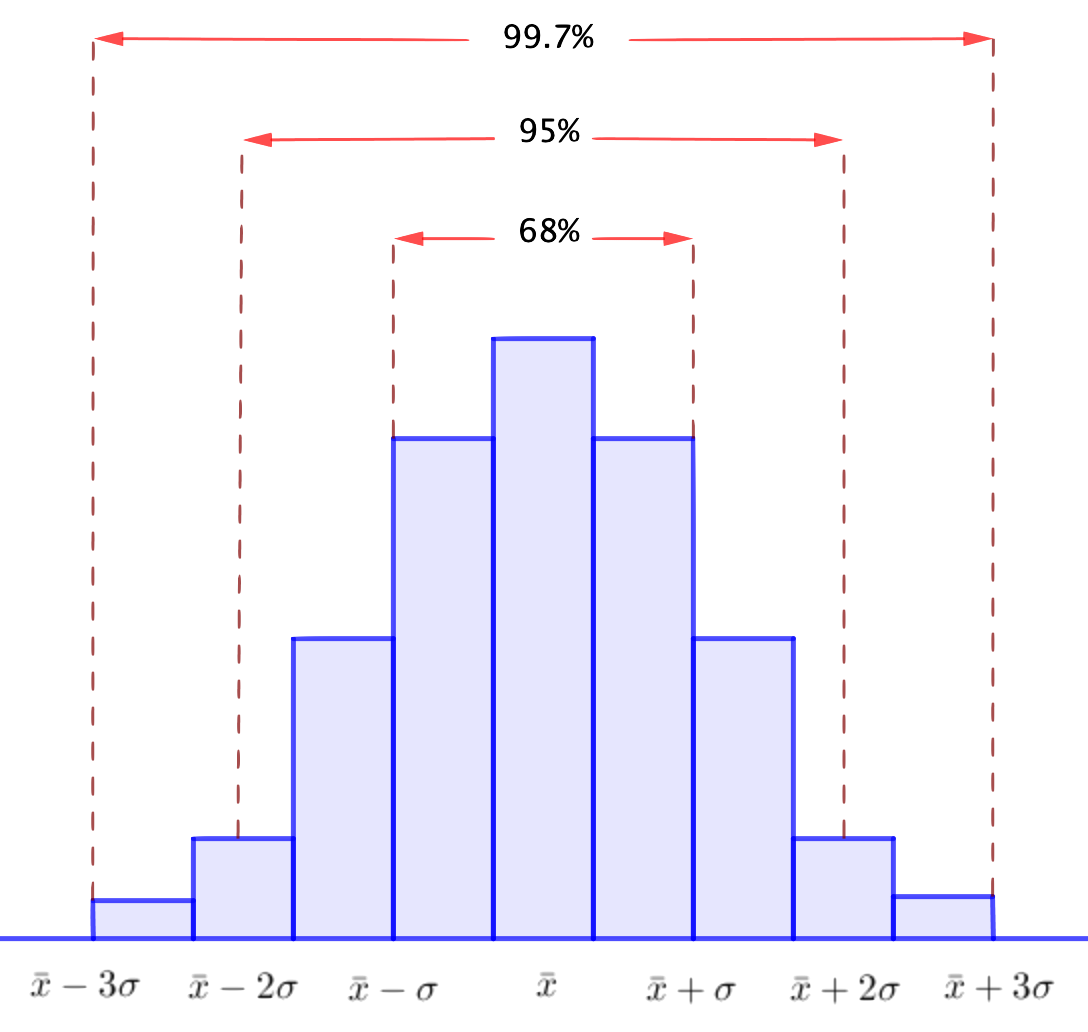
\includegraphics[width=.7\textwidth]{imagenes/imagenes01/T01IM21.png}
	\end{figure}
\end{myalertblock}

\section{Tipificación}

\begin{definition}
	
Haciendo uso de las propiedades de las medidas estadísticas, podremos facilitar y simplificar los cálculos de parámetros estadísticos mediante un cambio de variable.

\vspace{2mm} Así, si todos los valores son muy altos, podremos restarles una cantidad (normalmente la Moda) y, si poseen cifras decimales o son múltiplos de un mismo número, podremos multiplicarlos o dividirlos por el valor adecuado. 

\vspace{2mm} Una vez calculados los parámetros estadísticos, en virtud de las propiedades descritas, obtendremos el valor final real de tales parámetros. 

\vspace{2mm} Mención especial merecen dos cambio de variables particular : 

1.$\ $ \textbf{Diferenciales}: partiendo de la variable inicial $x_i$ (puntuaciones directas), si a todos los valores les restamos la media, obtenemos una nueva variable $y_i=x_i-\var x$ (puntuaciones diferenciales) cuya media es cero (la desviación típica no se modifica). 

2.$\ $  \textbf{Tipificadas}: Si a todos los valores de la variable inicial $x_i$ les restamos la media y el resultado lo dividimos por la desviación típica, obtenemos una nueva variable $\boldsymbol{z_i=\frac{x_i-\bar x}{s_x}}$, \emph{puntuaciones típicas o tipificadas} cuya media es cero y cuya  desviación típica es siempre la unidad. 

\vspace{2mm} Este último cambio de variable recibe el nombre de \textbf{TIPIFICACIÓN} y es muy útil a la hora de comparar dos valores de individuos pertenecientes a distribuciones distintas.
\end{definition}

\vspace{15mm}%**********************
\begin{example}

Un alumno obtiene en un examen de matemáticas una calificación de $8$ en un grupo cuya media es $5$ y desviación típica $1$. Su amigo, en otro grupo de media $6$ y desviación típica $2$ obtiene un $10$. ?`Cuál de las dos notas, comparativamente a su grupo, es mejor calificación?. 

\vspace{4mm} Nos encontramos con dos distribuciones de calificaciones medidas en distintas escalas. Para poder comparar tendremos que referir ambas series de valores a otras equivalentes entre sí (igual media y desviación típica). 

\vspace{2mm} El proceso de \emph{tipificación} nos proporciona lo que deseamos, siempre obtendremos una distribución con media $0$ y desviación típica $1$, donde los datos ya son comparables.
 
\vspace{2mm} Tipificando ambas calificaciones se obtiene :

\vspace{2mm} Nota del primer amigo: $\ z_i=\dfrac{8-5}{1}=3$

\vspace{2mm} Nota del segundo amigo: $z_2=\dfrac{10-6}{2}=2$ 

\vspace{2mm} La nota obtenida del primer amigo es, comparativamente,  superior a la del segundo. 
\end{example}

\newpage %********************************************
\section{Ejercicios}
	
\begin{ejemplo}
\begin{ejer}
	Considera las siguientes distribuciones:
	
\begin{table}[H]
\centering
\begin{tabular}{|r|r|r|r|r|}
\cline{1-2} \cline{4-5}
\multicolumn{2}{|c|}{\textbf{Distribución 1}} & \multicolumn{1}{c|}{\textbf{}} & \multicolumn{2}{c|}{\textbf{Distribución 2}} \\ \cline{1-2} \cline{4-5} 
\multicolumn{1}{|c|}{\textbf{clase}} & \multicolumn{1}{c|}{\textbf{$n_i$}} & \multicolumn{1}{c|}{\textbf{$\qquad$}} & \multicolumn{1}{c|}{\textbf{clase}} & \multicolumn{1}{c|}{\textbf{$n_i$}} \\ \cline{1-2} \cline{4-5} 
[10,20[ & 3 &  & [10,20[ & 5 \\ \cline{1-2} \cline{4-5} 
[20,30[ & 17 &  & [20,30[ & 9 \\ \cline{1-2} \cline{4-5} 
[30,40[ & 13 &  & [30,40[ & 23 \\ \cline{1-2} \cline{4-5} 
[40,50[ & 9 &  & [40,50[ & 9 \\ \cline{1-2} \cline{4-5} 
[50,60[ & 8 &  & [50,60[ & 4 \\ \cline{1-2} \cline{4-5} 
\end{tabular}
\end{table}	
\end{ejer}

$a)\quad$ Dibuja el histograma de cada distribución y deduce, de su observación, cuál de las dos distribuciones es más dispersa.

$b)\quad$ Calcula $mo, \ me, \ Q_1, D_1, P_{66}$ para la primera distribución.

$c)\quad$ Calcula $\bar x,\ \bar x_g, \bar x_a$ para la primera distribución.

$d)\quad$ Calcula el rango, la desviación media y la desviación típica, para la primera distribución.

$e)\quad$ Calcula los coeficientes de variación de Pearson para ambas distribuciones y deduce, a partir de ellos, cuál es la distribución más dispersa.

$f)\quad$ Da, para la primera distribución, una interpretación conjunta de media y desviación típica. ?`A partir de qué valor se está entre los 10\% valores más altos? ?`Cuántos valores hay menores que 47? 

$g)\quad$ Encuentra los coeficientes de asimetría y de curtosis de ambas distribuciones. ?`Qué puedes decir de la forma de estas distribuciones?.

$h)\quad$ Dibuja el diagrama de cajas y bigotes.

$i)\quad$ ?`Entre que valores se encuentra el 20\% de los valores centrales?

\end{ejemplo}

Cálculos:


\begin{table}[H]
\tiny
\centering
\begin{tabular}{rrrrrrrrr}
\multicolumn{8}{l}{\textbf{Distribución 1}} & \multicolumn{1}{l}{\textbf{}} \\ \hline
\multicolumn{1}{|c|}{\textbf{$x_i$}} & \multicolumn{1}{c|}{\textbf{$n_i$}} & \multicolumn{1}{c|}{\textbf{$N_i$}} & \multicolumn{1}{c|}{\textbf{$x_i \cdot n_i$}} & \multicolumn{1}{c|}{\textbf{$x_i-\bar x$}} & \multicolumn{1}{c|}{\textbf{$|x_i-\bar x|\cdot n_i$}} & \multicolumn{1}{c|}{\textbf{$(x_i-\bar x)^2\cdot n_i$}} & \multicolumn{1}{c|}{\textbf{$(x_i-\bar x)^3\cdot n_i$}} & \multicolumn{1}{c|}{\textbf{$(x_i-\bar x)^4\cdot n_i$}} \\ \hline
\multicolumn{1}{|r|}{15} & \multicolumn{1}{r|}{3} & \multicolumn{1}{r|}{3} & \multicolumn{1}{r|}{45} & \multicolumn{1}{r|}{-20.4} & \multicolumn{1}{r|}{61.2} & \multicolumn{1}{r|}{1248.48} & \multicolumn{1}{r|}{-25468.99} & \multicolumn{1}{r|}{519567.44} \\ \hline
\multicolumn{1}{|r|}{25} & \multicolumn{1}{r|}{17} & \multicolumn{1}{r|}{20} & \multicolumn{1}{r|}{425} & \multicolumn{1}{r|}{-10.4} & \multicolumn{1}{r|}{176.8} & \multicolumn{1}{r|}{1838.72} & \multicolumn{1}{r|}{-19122.69} & \multicolumn{1}{r|}{198875.96} \\ \hline
\multicolumn{1}{|r|}{35} & \multicolumn{1}{r|}{13} & \multicolumn{1}{r|}{33} & \multicolumn{1}{r|}{455} & \multicolumn{1}{r|}{-0.4} & \multicolumn{1}{r|}{5.2} & \multicolumn{1}{r|}{2.08} & \multicolumn{1}{r|}{-0.83} & \multicolumn{1}{r|}{0.33} \\ \hline
\multicolumn{1}{|r|}{45} & \multicolumn{1}{r|}{9} & \multicolumn{1}{r|}{42} & \multicolumn{1}{r|}{405} & \multicolumn{1}{r|}{9.6} & \multicolumn{1}{r|}{86.4} & \multicolumn{1}{r|}{829.44} & \multicolumn{1}{r|}{7962.62} & \multicolumn{1}{r|}{76441.19} \\ \hline
\multicolumn{1}{|r|}{55} & \multicolumn{1}{r|}{8} & \multicolumn{1}{r|}{50} & \multicolumn{1}{r|}{440} & \multicolumn{1}{r|}{19.6} & \multicolumn{1}{r|}{156.8} & \multicolumn{1}{r|}{3073.28} & \multicolumn{1}{r|}{60236.29} & \multicolumn{1}{r|}{1180631.24} \\ \hline
\multicolumn{1}{r|}{\textbf{}} & \multicolumn{1}{r|}{\textbf{N=50}} & \multicolumn{1}{r|}{\textbf{}} & \multicolumn{1}{r|}{\textbf{1770}} & \multicolumn{1}{r|}{\textbf{}} & \multicolumn{1}{r|}{\textbf{486.4}} & \multicolumn{1}{r|}{\textbf{6992.00}} & \multicolumn{1}{r|}{\textbf{23606.40}} & \multicolumn{1}{r|}{\textbf{1975516.16}} \\ \cline{2-2} \cline{4-4} \cline{6-9} 
\end{tabular}
\end{table}

\begin{table}[H]
\tiny
\centering
\begin{tabular}{rrrrrrrrr}
\multicolumn{8}{l}{\textbf{Distribución 2}} & \multicolumn{1}{l}{\textbf{}} \\ \hline
\multicolumn{1}{|c|}{\textbf{$x_i$}} & \multicolumn{1}{c|}{\textbf{$n_i$}} & \multicolumn{1}{c|}{\textbf{$N_i$}} & \multicolumn{1}{c|}{\textbf{$x_i \cdot n_i$}} & \multicolumn{1}{c|}{\textbf{$x_i-\bar x$}} & \multicolumn{1}{c|}{\textbf{$|x_i-\bar x|\cdot n_i$}} & \multicolumn{1}{c|}{\textbf{$(x_i-\bar x)^2\cdot n_i$}} & \multicolumn{1}{c|}{\textbf{$(x_i-\bar x)^3\cdot n_i$}} & \multicolumn{1}{c|}{\textbf{$(x_i-\bar x)^4\cdot n_i$}} \\ \hline
\multicolumn{1}{|r|}{15} & \multicolumn{1}{r|}{5} & \multicolumn{1}{r|}{5} & \multicolumn{1}{r|}{75} & \multicolumn{1}{r|}{-19.6} & \multicolumn{1}{r|}{98} & \multicolumn{1}{r|}{1920.8} & \multicolumn{1}{r|}{-37647.68} & \multicolumn{1}{r|}{737894.53} \\ \hline
\multicolumn{1}{|r|}{25} & \multicolumn{1}{r|}{9} & \multicolumn{1}{r|}{14} & \multicolumn{1}{r|}{225} & \multicolumn{1}{r|}{-9.6} & \multicolumn{1}{r|}{86.4} & \multicolumn{1}{r|}{829.44} & \multicolumn{1}{r|}{-7962.62} & \multicolumn{1}{r|}{76441.19} \\ \hline
\multicolumn{1}{|r|}{35} & \multicolumn{1}{r|}{23} & \multicolumn{1}{r|}{37} & \multicolumn{1}{r|}{805} & \multicolumn{1}{r|}{0.4} & \multicolumn{1}{r|}{9.2} & \multicolumn{1}{r|}{3.68} & \multicolumn{1}{r|}{1.47} & \multicolumn{1}{r|}{0.59} \\ \hline
\multicolumn{1}{|r|}{45} & \multicolumn{1}{r|}{9} & \multicolumn{1}{r|}{46} & \multicolumn{1}{r|}{405} & \multicolumn{1}{r|}{10.4} & \multicolumn{1}{r|}{93.6} & \multicolumn{1}{r|}{973.44} & \multicolumn{1}{r|}{10123.78} & \multicolumn{1}{r|}{105287.27} \\ \hline
\multicolumn{1}{|r|}{55} & \multicolumn{1}{r|}{4} & \multicolumn{1}{r|}{50} & \multicolumn{1}{r|}{220} & \multicolumn{1}{r|}{20.4} & \multicolumn{1}{r|}{81.6} & \multicolumn{1}{r|}{1664.64} & \multicolumn{1}{r|}{33958.66} & \multicolumn{1}{r|}{692756.58} \\ \hline
\multicolumn{1}{r|}{\textbf{}} & \multicolumn{1}{r|}{\textbf{N=50}} & \multicolumn{1}{r|}{\textbf{}} & \multicolumn{1}{r|}{\textbf{1730}} & \multicolumn{1}{r|}{\textbf{}} & \multicolumn{1}{r|}{\textbf{368.8}} & \multicolumn{1}{r|}{\textbf{5392.00}} & \multicolumn{1}{r|}{\textbf{-1526.40}} & \multicolumn{1}{r|}{\textbf{1612380.16}} \\ \cline{2-2} \cline{4-4} \cline{6-9} 
\end{tabular}
\end{table}

Para el cálculo de las desviaciones es necesario, previamente, calcular la medias:

\vspace{-4mm}%***********************************
$$\bar x_1=\dfrac{1770}{50}=34,5; \qquad \bar x_2=\dfrac{1730}{50}=34,6$$

\textcolor{blue}{------ $a)\ $  Histogramas:}
\begin{figure}[H]
			\centering
			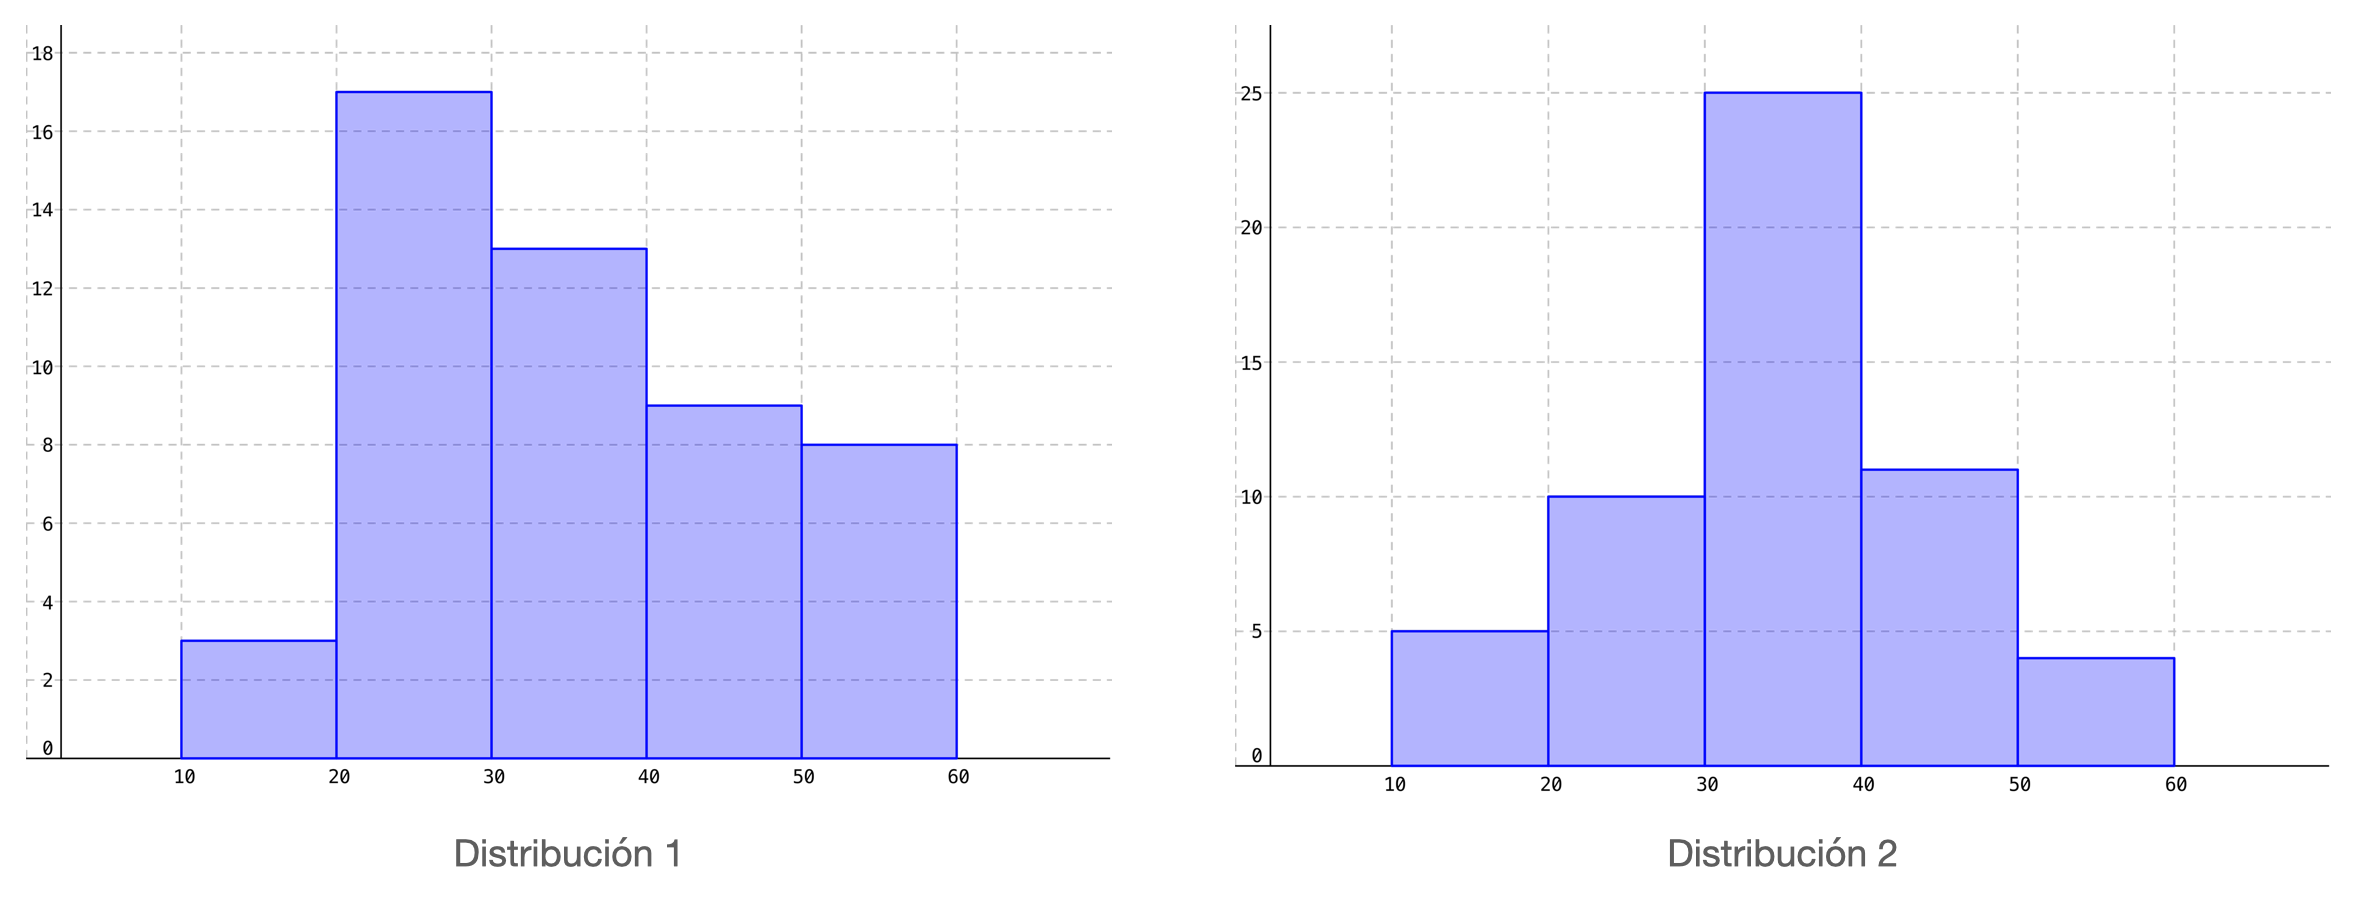
\includegraphics[width=.9\textwidth]{imagenes/imagenes01/T01IM22.png}
	\end{figure}


\vspace{-4mm} %******************************************
A simple vista, la distribución 1 parece más dispersa que la distribución 2. En el apartado $e)$ lo veremos con más precisión al calcular los respectivos coeficientes de variación (Pearson). 
	
\textcolor{blue}{------ $b)\  mo, me, Q_1, D_1, P_{66}$ para la primera distribución:}

El intervalo modal, de mayor frecuencia absoluta, es el $[20,30[$, su frecuencia absoluta es $n_k=17$ y las frecuencias absolutas de los intervalos anterior y posterior	son, respectivamente, $m_{k-1}=3$ y $n_{k+1}=13$. La amplitud del intervalo modal es $c_k=10$, como la de todos ellos.
	
$\Rightarrow \quad mo=20+\dfrac{17-3}{(17-3)+(17-13)}\ 10=27.8$

\vspace{5mm} %******************
{\color{gris}\hrule} 
\begin{multicols}{2}
Calculamos la moda sin usar la fórmula:

Los triángulos $AOB \sim DOE$ son \emph{semejantes}.

$\dfrac{AB}{OC}=\dfrac{DE}{OF}$

$\dfrac{14}{x}=\dfrac{4}{10-x}$

$x=7.8 \Rightarrow $



$\qquad mo=20+7.8=27.8$

\begin{figure}[H]
			\centering
			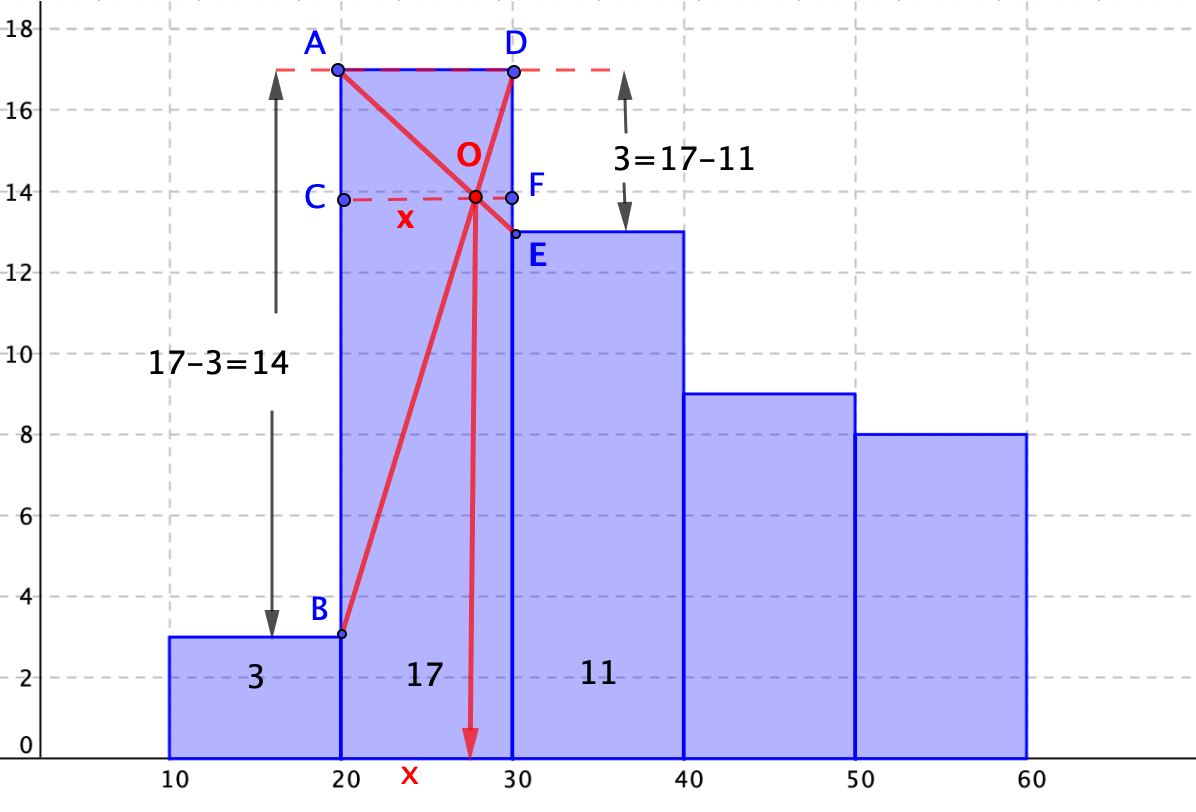
\includegraphics[width=.5\textwidth]{imagenes/imagenes01/T01IM23.png}
	\end{figure}
\end{multicols}
{\color{gris}\hrule}

\vspace{5mm} %*******************************
El intervalo mediano es el tercero, $[30,40[$ de frecuencia absoluta $n_k=13$ y cuya frecuencia acumulada del intervalo anterior es $N_{k-1}=20$. La amplitud de éste y todos los intervalos en $c_k=10$.

$\Rightarrow \quad  me=30+\dfrac{\dfrac{50}{2}-20}{13}\ 10=33.8$


\vspace{10mm}
{\color{gris}\hrule}
\begin{multicols}{2}
Calculamos la mediana sin usar la fórmula:

Los triángulos $AOB \sim ADC$ 

son \emph{semejantes}.

$\quad$

$\dfrac{OB}{AB}=\dfrac{DC}{AC}$

$\dfrac{5}{x}=\dfrac{13}{10}$

$x=3.8 \Rightarrow $

$\qquad  mo=30+3.8=33.8$

\begin{figure}[H]
			\centering
			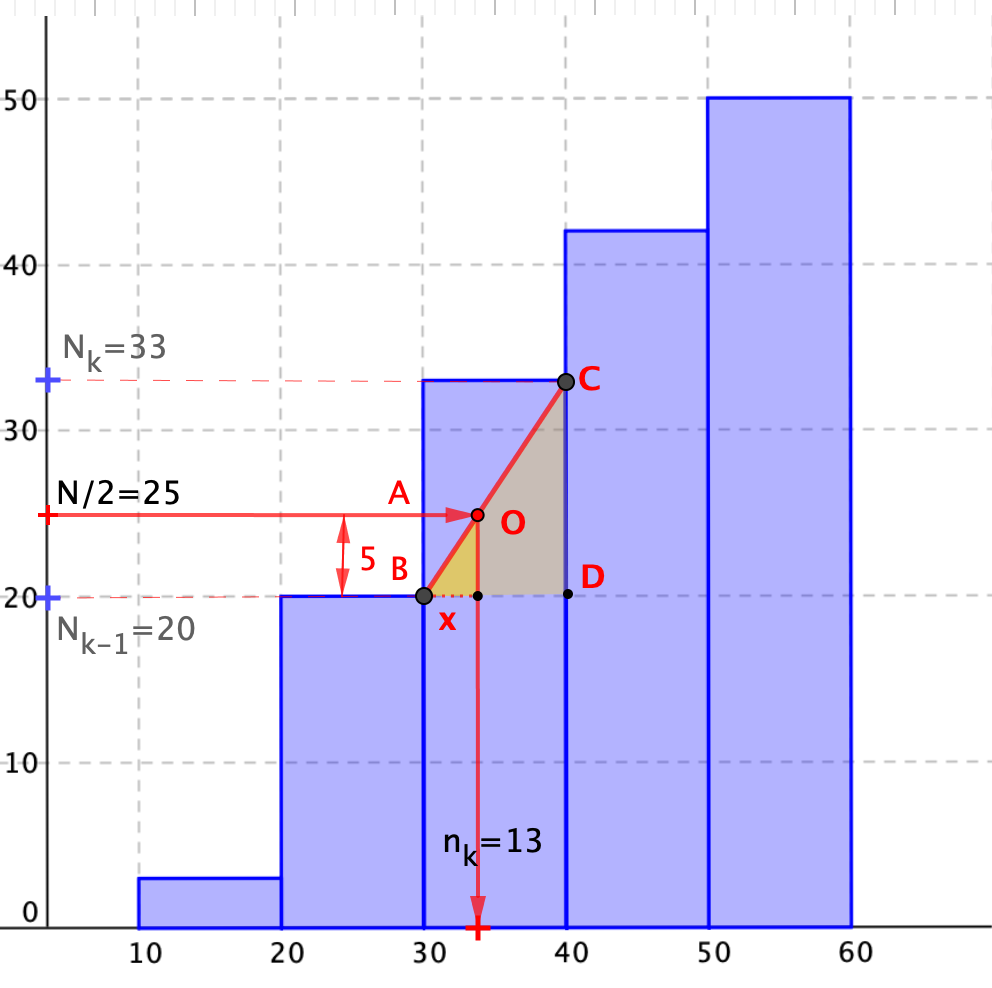
\includegraphics[width=.4\textwidth]{imagenes/imagenes01/T01IM24.png}
	\end{figure}
\end{multicols}

{\color{gris}\hrule}
	
\vspace{4mm} %*******************************

$\Rightarrow \quad  25\% (50)=12.5 \to Q_1=20+ \dfrac{12.5-3}{17}\ 10=25.6$

$\Rightarrow \quad 10\% (50)=5 \to D_1=20+\dfrac{5-3}{17}\ 10=21.2$

$\Rightarrow \quad 65\% (50)=32.5 \to P_{66}=30+\dfrac{32.5-20}{13}\ 10=39.6$

\textcolor{blue}{------ $c)\ \bar x,\ \bar x_g,\ \bar x_a$ de distribución-1.}

\begin{table}[H]
\footnotesize
\centering
\begin{tabular}{rrrrr}
\multicolumn{1}{l}{\textbf{Distribución 1}} & \multicolumn{1}{l}{\textbf{}} & \multicolumn{1}{l}{\textbf{}} & \multicolumn{1}{l}{\textbf{}} & \multicolumn{1}{l}{\textbf{}} \\ \hline
\multicolumn{1}{|c|}{\textbf{$x_i$}} & \multicolumn{1}{c|}{\textbf{$n_i$}} & \multicolumn{1}{c|}{\textbf{$x_i \cdot n_i$}} & \multicolumn{1}{c|}{\textbf{${x_i}^{n_i}$}} & \multicolumn{1}{c|}{\textbf{$n_i / x_i$}} \\ \hline
\multicolumn{1}{|r|}{15} & \multicolumn{1}{r|}{3} & \multicolumn{1}{r|}{45} & \multicolumn{1}{r|}{3.30E+03} & \multicolumn{1}{r|}{0.20} \\ \hline
\multicolumn{1}{|r|}{25} & \multicolumn{1}{r|}{17} & \multicolumn{1}{r|}{425} & \multicolumn{1}{r|}{5.82E+23} & \multicolumn{1}{r|}{0.68} \\ \hline
\multicolumn{1}{|r|}{35} & \multicolumn{1}{r|}{13} & \multicolumn{1}{r|}{455} & \multicolumn{1}{r|}{1.18E+20} & \multicolumn{1}{r|}{0.37} \\ \hline
\multicolumn{1}{|r|}{45} & \multicolumn{1}{r|}{9} & \multicolumn{1}{r|}{405} & \multicolumn{1}{r|}{7.57E+14} & \multicolumn{1}{r|}{0.20} \\ \hline
\multicolumn{1}{|r|}{55} & \multicolumn{1}{r|}{8} & \multicolumn{1}{r|}{440} & \multicolumn{1}{r|}{8.37E+13} & \multicolumn{1}{r|}{0.15} \\ \hline
\multicolumn{1}{r|}{\textbf{}} & \multicolumn{1}{r|}{\textbf{N=50}} & \multicolumn{1}{r|}{\textbf{1770}} & \multicolumn{1}{r|}{\textbf{$\Pi=\ $ 1.47E+76}} & \multicolumn{1}{r|}{\textbf{1.60}} \\ \cline{2-5} 
\end{tabular}
\end{table}

$\bar x=\dfrac {1770}{50}=35.4;\quad \bar x_g=\sqrt[50]{1.47\times 10^{76}}=33.4;\quad \bar x_a =\dfrac{50}{1.60}=31.3$

\textcolor{blue}{------ $d)\ R,\ DM,\ s$ ,  de distribución-1.}

$\Rightarrow \quad R=60-10=50$

$\Rightarrow \quad DM=\dfrac{486.4}{50}=9.7$

$\Rightarrow \quad s=\sqrt{\dfrac{6992.00}{50}}=11.83$

\textcolor{blue}{------ $e)\ $ CV para ambas distribuciones:}

$\bar x_1=35.5;\ \ s_1=11.83; \qquad x_2=34.6; \ \ s_2=\sqrt{\dfrac{5392}{50}}=10.38$

$\Rightarrow \quad CV_1=\dfrac{\bar s_1}{x_1}=0.343=34.3\%$

$\Rightarrow \quad CV_2=\dfrac{\bar s_2}{x_2}=0.300=30.0\%$

Como habíamos predicho en el apartado $\ a)\ $ la primera distribución tiene los datos más dispersos.

\textcolor{blue}{------ $f)\ n_i \in [\bar x-\sigma, \bar x+\sigma];\ \ \ 10\% \uparrow \to P_90; \ \ \ $ ?`cuantos individuos tiene $x_i<47$?.} 

En el intervalo $ [\bar x-\sigma, \bar x+\sigma]=[22.67,46,33]$ están todos los individuos del intervalo $[30,40[$, esto es, $\underline {13}$ individuos más la parte proporcional de individuos de cada uno de los intervalos adyacentes. 

En $[20,30[$ hay $17$ individuos, para una amplitud de $10$. En $[22.67,30[$, de amplitud $7.33$ habrán:  $17\ \frac{7.33}{10}=\underline{12.46}$

$\Rightarrow \quad $ En $[40,50[$ hay $9$ individuos, para una amplitud de $10$. En $[40,46.33[$, de amplitud $6.33$ habrán:  $9\ \frac{6.33}{10}=\underline{5.70}$

Por lo que, en $ [\bar x-\sigma, \bar x+\sigma]=[22.67,46,33]$  hay $12.46+13+5.70=31,16$, lo que significa una proporción del $\dfrac{31.16}{50}=62.32\%$ de la población. \textcolor{gris}{(Esta el la interpretación conjunta de media y desviación típica).}

Estar entre el 10\% de los individuos de mayor puntuación es lo mismo que dejar atrás al 90\% de ellos, nos piden en percentil 90.

$90\%(50)=45 \to P_{90}$ estamos en el último intervalo:

$\Rightarrow \quad P_{90}= 50+\dfrac{45-42}{8}\ 10=53.7$

$47 \in [40,50]$ luego con $x_i<47$ estarán todos los individuos de los intervalos anteriores, $3+17+13$, y la parte proporcional de los $9$ individuos del intervalo de amplitud $10, [40,50[$:

$\Rightarrow \quad 3+17+13+ \frac{47-40}{9} \ 10 =40.78$, hay 40 individuos con puntuación menor que $47$. 
 
\textcolor{blue}{------ $g) \ As_1,\ K_1;\ \ \ As_2,\ K_2$}

\begin{multicols}{2}
$As_1=\dfrac{23606.40}{50\dot 11.83^3}=3.51$

$K_1=\dfrac{1975516.16}{50\cdot 11.83^4}-3=-0.98$

$As_2=\dfrac{-1526.40}{50\dot 10.38^3}=-0.03$

$K_2=\dfrac{1612380.16}{50\cdot 10.38^4}-3=-0.22$
\end{multicols}

La primera distribución está sesgada a la derecha (positivamente) y más platicúrtica que la segunda.


\textcolor{blue}{------ $g) \ $  Diagrama de cajas y bigotes.}

En apartados anteriores obtuvimos: $\ me=33.8;\ \ Q_1=25.6;\ \ x_{min}=10;\ \ x_{max}=60$

$75\% (50)=37.5 \ \to \ Q_3=40+\dfrac{37.5-33}{9}\ 10=45.0$

Valores atípicos: $Lim_{inf}=25.6-3\ \dfrac{45-25.6}{2}=-17.0$; $Lim_{sup}=45.0-3\ \dfrac{45-25.6}{2}=87.6$

Fuera del intervalo $]-17.0,87.6[$ no hay ningún valor, por lo que no existen valores atípicos para esta distribución.

Diagrama de cajas y bigotes:

\begin{figure}[H]
			\centering
			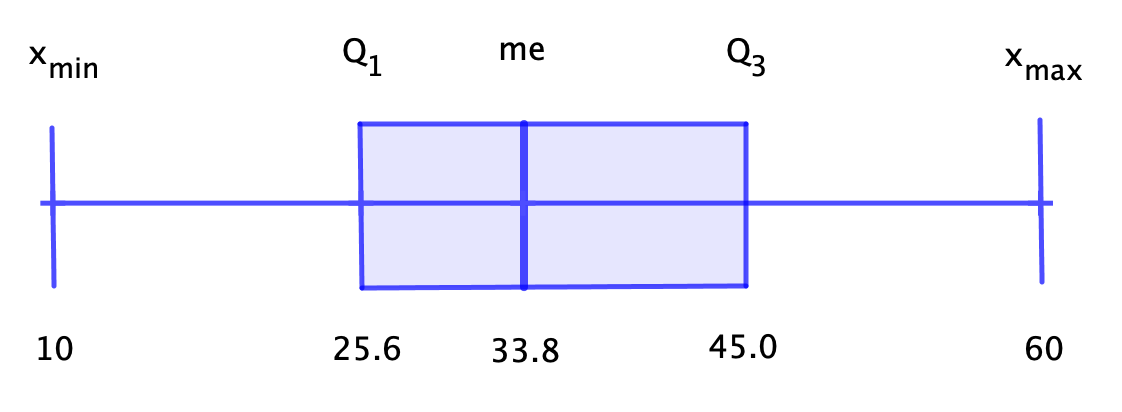
\includegraphics[width=.5\textwidth]{imagenes/imagenes01/T01IM39.png}
	\end{figure}

Se observa un cierto sesgo a la derecha.

\textcolor{blue}{------ $i)\ ]P_{40},P_{60}[$}

El valor central es la mediana, el $P_{50}$; el $20\%$ de los valores a su alrededor estarán comprendidos entre el $P_{40}$ y el $P_{60}$

$40\%(40)=20 \ \to \ P_{40}=30$

$60\%(40)=30 \ \to \ P_{60}=30+\dfrac{30-20}{13}\ 10=37.69$

El intervalo pedido es $\ [30,37.69]$

\vspace{5mm}%********************************
\begin{ejemplo}
\begin{ejer}
	Para los datos 7, 3, 4, 6, 4, 3, 3; calcula la media artimética, geométrica y armónica.
\end{ejer}	
\end{ejemplo}

\begin{table}[H]
\centering
\begin{tabular}{rrrrr}
\multicolumn{1}{c}{\textbf{$x_i$}} & \multicolumn{1}{c}{\textbf{$n_i$}} & \multicolumn{1}{c}{\textbf{$x_i\ n_i$}} & \multicolumn{1}{c}{\textbf{$x_i^{n_i}$}} & \multicolumn{1}{c}{\textbf{$n_1/x_i$}} \\ \hline
\multicolumn{1}{|r|}{3} & \multicolumn{1}{r|}{3} & \multicolumn{1}{r|}{9} & \multicolumn{1}{r|}{27} & \multicolumn{1}{r|}{1.00} \\ \hline
\multicolumn{1}{|r|}{4} & \multicolumn{1}{r|}{2} & \multicolumn{1}{r|}{8} & \multicolumn{1}{r|}{16} & \multicolumn{1}{r|}{0.50} \\ \hline
\multicolumn{1}{|r|}{6} & \multicolumn{1}{r|}{1} & \multicolumn{1}{r|}{6} & \multicolumn{1}{r|}{6} & \multicolumn{1}{r|}{0.17} \\ \hline
\multicolumn{1}{|r|}{7} & \multicolumn{1}{r|}{1} & \multicolumn{1}{r|}{7} & \multicolumn{1}{r|}{7} & \multicolumn{1}{r|}{0.14} \\ \hline
\multicolumn{1}{l|}{} & \multicolumn{1}{l|}{$N=8$} & \multicolumn{1}{l|}{$\Sigma \to 30$} & \multicolumn{1}{l|}{$\Pi \to 18144$} & \multicolumn{1}{l|}{$\sigma \to 1.81$} \\ \cline{2-5} 
\end{tabular}
\end{table}

$\bar x=\dfrac{\displaystyle \sum_{i=1}^4 x_i \cdot n_i}{N}=3.75; \quad$
$\bar x_g=\sqrt[8] {\displaystyle \prod_{i=1}^4 x_i^{n_i}}=3.41; \quad$
$\bar x_a=\dfrac{N}{\displaystyle \sum_{i=1}^4 \dfrac{n_i}{x_i} }=4.42$

\vspace{0.5mm} %**********************
\begin{destacado}
Diferencia entra variable discreta y continua a la hora del cálculo de parámetros de posición. 

En variable discreta para encontrar la posición del individuo adecuado usaremos una aproximación por defecto.	
\end{destacado}

\vspace{5mm}%********************************
\begin{ejemplo}
\begin{ejer}
	Para las dos siguientes distribuciones, encontrar el $P_{33}$
	
\begin{table}[H]
\centering
\begin{tabular}{r|r|rrrr|r|r}
\cline{1-3} \cline{5-8}
\multicolumn{3}{|c|}{\textbf{Distribución 1}} & \multicolumn{1}{c|}{\textbf{}} & \multicolumn{4}{c|}{\textbf{Distribución 2}} \\ \cline{1-3} \cline{5-8} 
\multicolumn{1}{|c|}{\textbf{$x_i$}} & \multicolumn{1}{c|}{\textbf{$n_i$}} & \multicolumn{1}{c|}{\textbf{$N_i$}} & \multicolumn{1}{c|}{\textbf{$\qquad$}} & \multicolumn{1}{c|}{\textbf{clase}} & \multicolumn{1}{c|}{\textbf{$x_i$}} & \multicolumn{1}{c|}{\textbf{$n_i$}} & \multicolumn{1}{c|}{\textbf{$N_i$}} \\ \cline{1-3} \cline{5-8} 
\multicolumn{1}{|r|}{3} & 3 & \multicolumn{1}{r|}{3} & \multicolumn{1}{r|}{} & \multicolumn{1}{r|}{[2,4[} & 3 & 3 & \multicolumn{1}{r|}{3} \\ \cline{1-3} \cline{5-8} 
\multicolumn{1}{|r|}{5} & 10 & \multicolumn{1}{r|}{10} & \multicolumn{1}{r|}{} & \multicolumn{1}{r|}{[4,6[} & 5 & 10 & \multicolumn{1}{r|}{10} \\ \cline{1-3} \cline{5-8} 
\multicolumn{1}{|r|}{7} & 15 & \multicolumn{1}{r|}{25} & \multicolumn{1}{r|}{} & \multicolumn{1}{r|}{[6,8[} & 7 & 15 & \multicolumn{1}{r|}{25} \\ \cline{1-3} \cline{5-8} 
\multicolumn{1}{|r|}{9} & 7 & \multicolumn{1}{r|}{35} & \multicolumn{1}{r|}{} & \multicolumn{1}{r|}{[8,10[} & 9 & 7 & \multicolumn{1}{r|}{35} \\ \cline{1-3} \cline{5-8} 
\multicolumn{1}{c|}{} & \multicolumn{1}{c|}{N=35} & \multicolumn{1}{c}{} & \multicolumn{1}{c}{} & \multicolumn{1}{c}{} & \multicolumn{1}{c|}{} & \multicolumn{1}{c|}{N=25} & \multicolumn{1}{c}{} \\ \cline{2-2} \cline{7-7}
\end{tabular}
\end{table}
\end{ejer}	
\end{ejemplo}

Para la distribución 1: $\ 33\%(35)=11.55 \to 12^o$ individuo deja tras de sí al (más) 33\% de los individuos de la población.

El valor de la variable para este $12^o$ individuo es $ \ P_33=7$

Para la distribución 2: $\ 33\%(35)=11.55 \to P_{33}=6+\dfrac{11.55-10}{15}\ 2=6.21$

\vspace{5mm}%********************************
\begin{ejemplo}
\begin{ejer}
	Una varable estadística $X$ tiene una media $\bar x=20$ y una desviación típica $s_x=5$. Si elevamos al cuadrado todos los datos, ?`cuál será ahora el valor de la media?
\end{ejer}	
\end{ejemplo}

$x_i \to y_i=x_i^2 \ \Rightarrow \  s_x^2=\dfrac{\displaystyle \sum n_i\cdot x_i^2}{N}- {\bar x}^2=\bar y-{\bar x}^2$

$\bar y={\bar x}^2+s^2x \ \to \ \bar y=20^2+5^2=425$


\vspace{5mm}%********************************
\begin{ejemplo}
\begin{ejer}
	Una variable estadística tiene $\bar x=8$ y $s_x=2$. ?`Qué transformación hay que hacer a la variable para que su nueva media sea $\bar y=42$ y la nueva desviación típica $s_y=10$
\end{ejer}	
\end{ejemplo}

El cambio lineal general es: $y_i=a+bx_i \ \vee \ Y=a+bX$
 
$\begin{cases}
\bar y &= a + bx \\
s_y &= bs_x	
\end{cases}
\to 
\begin{cases}
42&=a+8b\\ 10&=2b	
\end{cases} \to b=5;\  a=2 \ \Rightarrow \ Y=2+5X \ \ \ \textcolor{gris}{or\ y_i=2+5x_i}$


\vspace{5mm} %************************
\begin{ejemplo}
\begin{ejer}
Calcula la tasa covid 14 días para todo el territorio español $\to$ \textsf{``media ponderada''}.
	

	\begin{figure}[H]
			\centering
			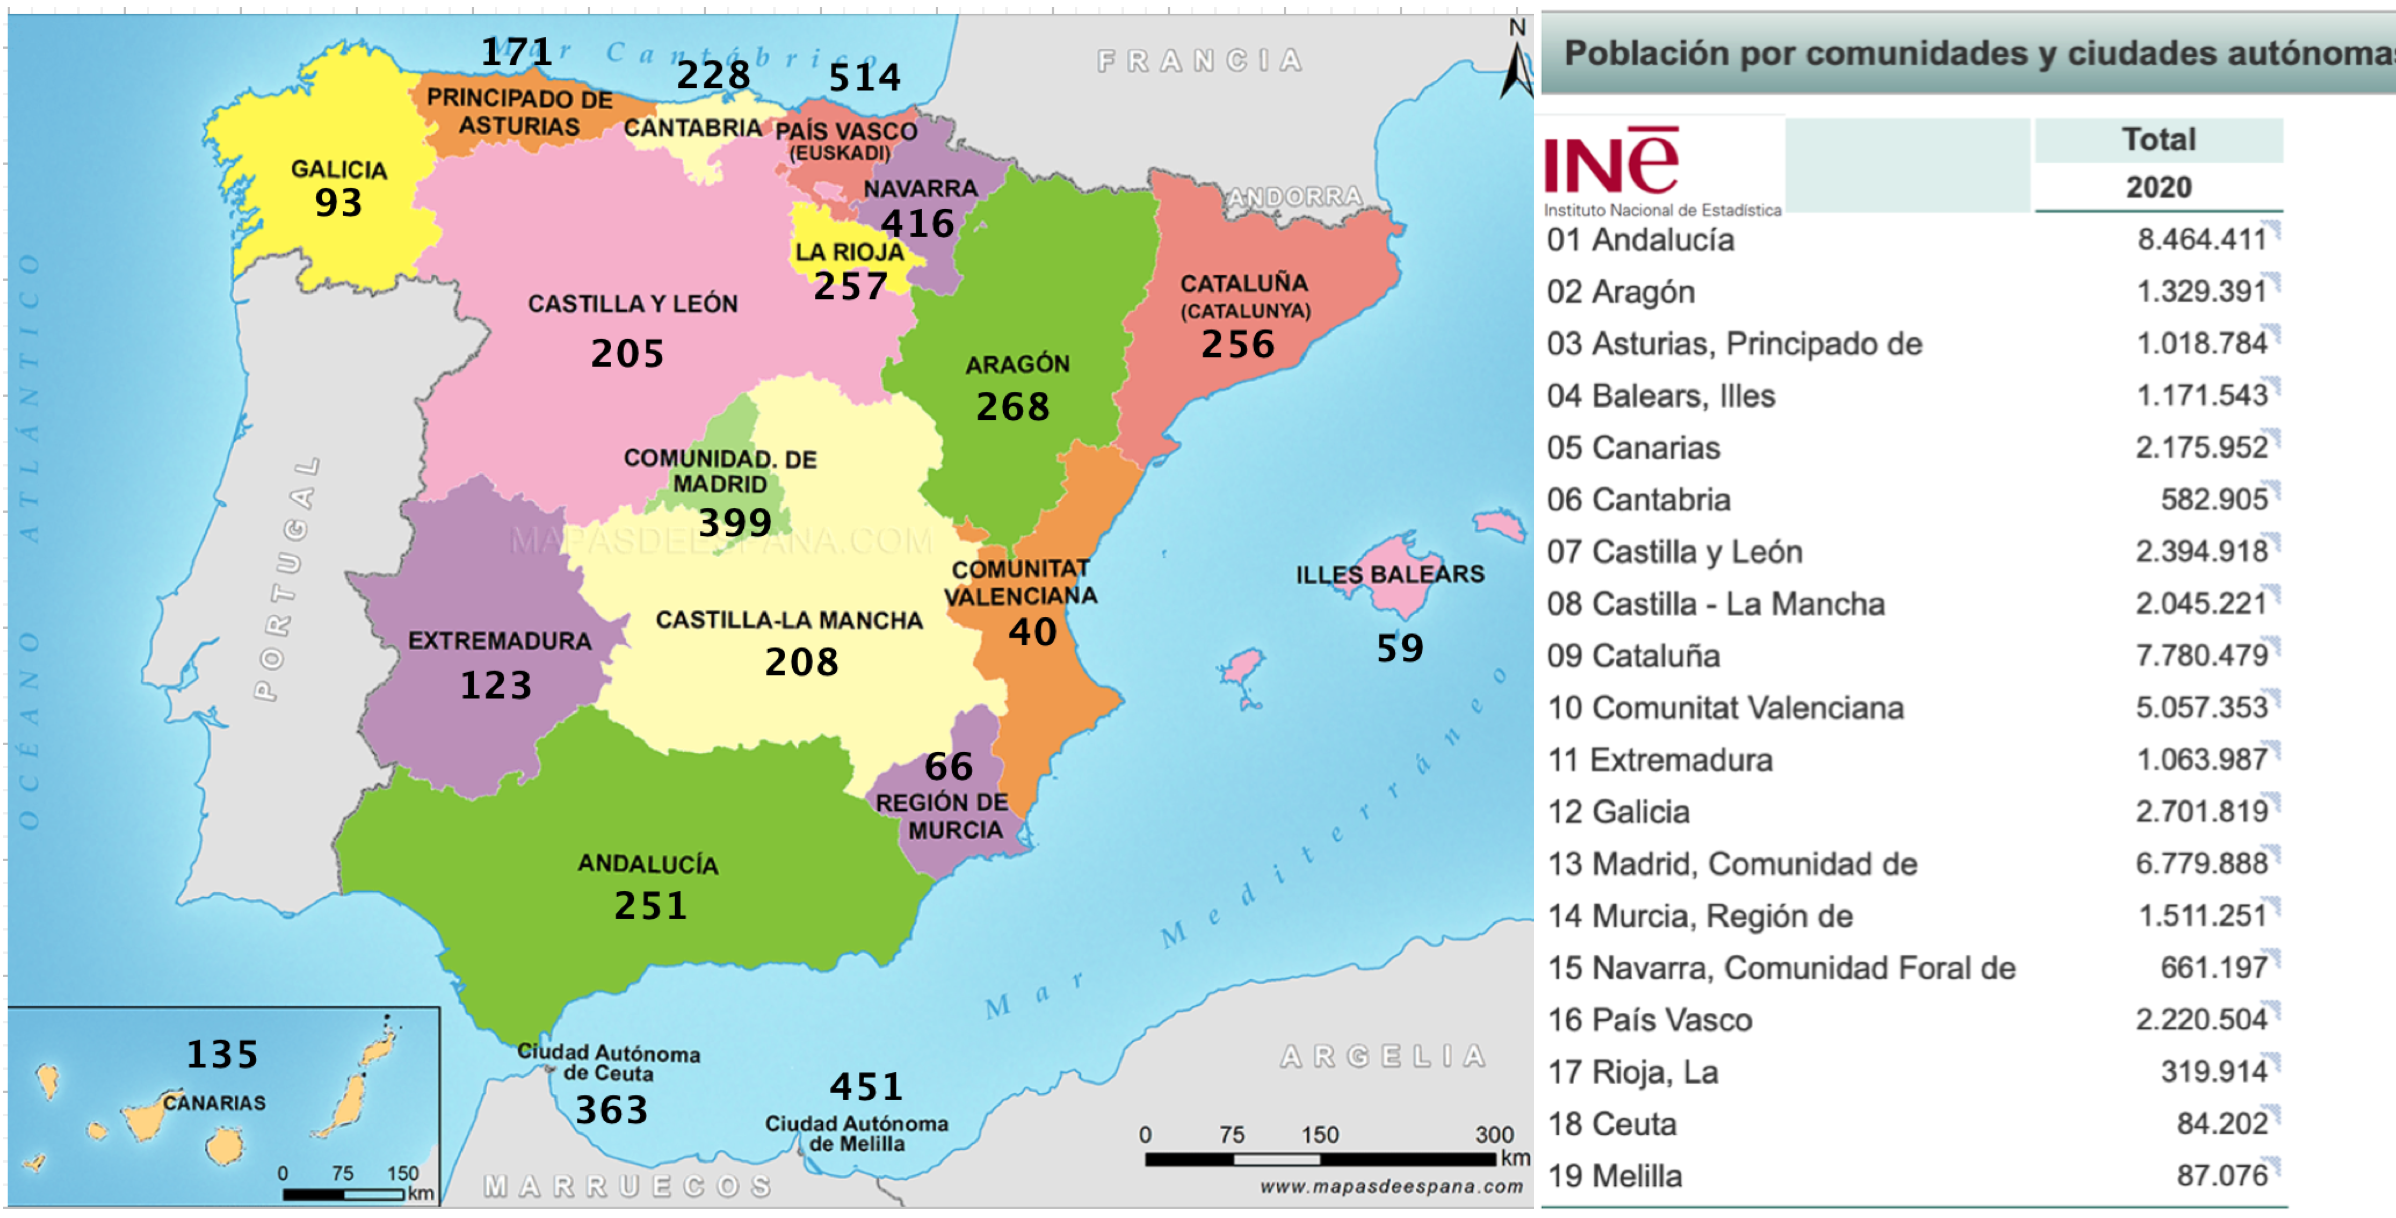
\includegraphics[width=1\textwidth]{imagenes/imagenes01/T01IM40.png}
	\end{figure}
\end{ejer}	
\end{ejemplo}

En el mapa (cartograma) aparece la incidencia acumulada de contagios en 14-días por cada 100.000 habitantes, a la derecha se muestra la población de cada comunidad autónoma.

Tomaremos como variable $x_i$ la incidencia acumulada por 100K habitantes de cada una de las 19 comunidades y ciudades autónomas de España y como frecuencia absoluta de cada una, $n_i$, la población. Así,

$\bar x_p=\displaystyle \sum_{i=1}^{19} x_i \cdot n_i \ / \  \sum_{i=1}^{19} n_i = 232.2$

\begin{destacado}
\emph{Todo lo visto en este tema se puede hacer, más rápidamente, con el múltiple sw existente, pero se ha optado por presentar todos los cálculos a mano por motivos didácticos.}
\end{destacado}




\section{Curiosidades}

\begin{myexampleblock}{Cómo mentir con estadísticas}

\emph{``Hay tres tipos de mentiras: mentiras, malditas mentiras y estadísticas’’}\footnote{Basado en el artículo de Francisco J. Lastra}; popularizada en los Estados Unidos por Mark Twain, esta frase describe el abuso de estadísticas para reforzar argumentos falaces.

\vspace{2mm} Un buen gráfico permite sintetizar información numérica, es difícil no convencerse de cualquier cosa cuando se acompaña la idea con gráficos. 

\vspace{2mm} La misma información se puede utilizar para crear dos gráficos con mensajes totalmente opuestos. Detrás de una estadística hay, sin duda, mucho más allá que figuras representativas de números, y es debido a esto que hoy existen expertos en el ``entendimiento de riesgo’’, estadísticos que trabajan con matemáticos, psicólogos y otros profesionales para transmitir al público de forma precisa sus hallazgos.

\vspace{2mm} ``Los gráficos pueden ser tan manipuladores como las palabras’’, por eso, ser capaces de leer, entender y evaluar estadísticas es una habilidad fundamental y estar atentos a los trucos que pueden hacernos caer en un error o engaño es una necesidad.

\vspace{2mm} Algunos casos de mentiras estadísticas, que rescatan los matemáticos Andrew Gelman y Deborah Nolan en su libro Teaching Statistics: A Bag of Tricks, son:

\vspace{2mm} \textbf{1. Inventar cifras}

\vspace{2mm} Según un estudio de la Universidad de Cambridge, un 53,4\% de las estadísticas son inventadas. Suena inteligente,¿`no?. Inventar estadísticas es la forma más directa de engaño de la que hablaremos y es, lamentablemente, más común de lo que se pensaría, gracias al aura de verdad o seriedad que un porcentaje o un grupo de barras puede darle al mensaje que lo acompaña.

\vspace{2mm} Uno de los ejemplos más recientes y notables por su impacto, y que afortunadamente fue desbaratado con rapidez, fue un tuit publicado por el candidato republicano Donald Trump.

\vspace{2mm} En diciembre del año pasado, Trump retuiteó estadísticas que señalaban, entre otras cosas, que un 81\% de los asesinatos de gente blanca era cometidos por gente negra.

\begin{multicols}{2}
	\begin{figure}[H]
			\centering
			
\includegraphics[width=.5\textwidth]{imagenes/imagenes01/T01IM30.png}
	\end{figure}
	
	\begin{figure}[H]
			\centering
			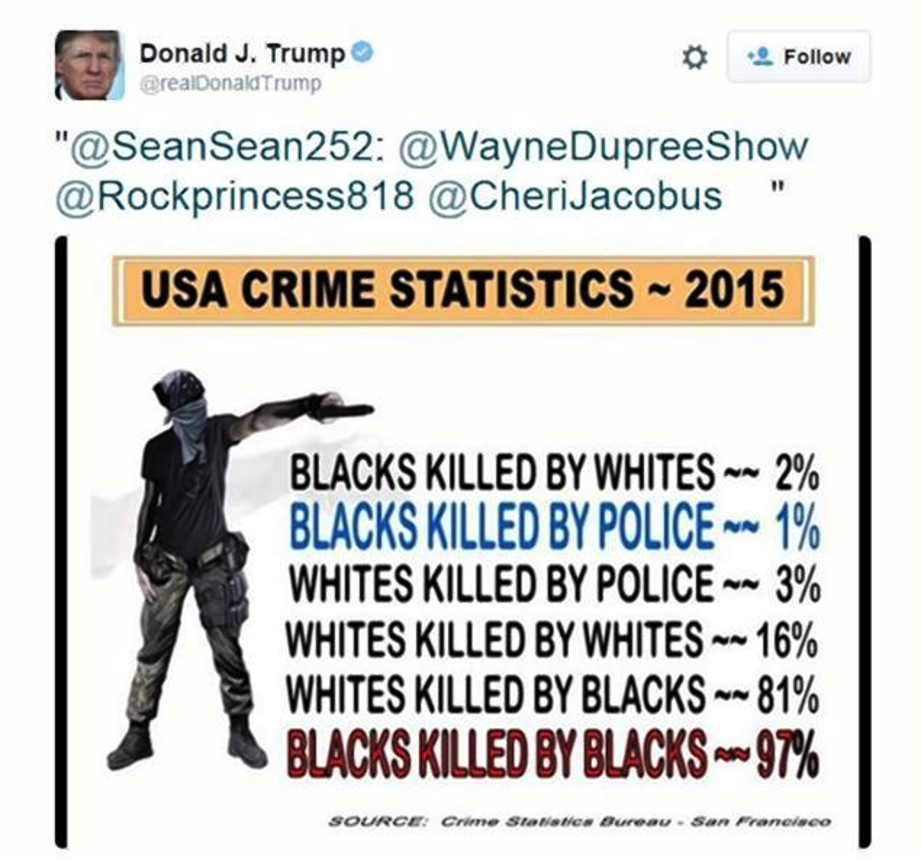
\includegraphics[width=.5\textwidth]{imagenes/imagenes01/T01IM31.png}
	\end{figure}
\end{multicols}


\vspace{2mm} Una rápida consulta de las cifras oficiales del FBI arrojó que el porcentaje, en realidad, asciende a un 15\% y que la supuesta fuente, la Oficina de Estadísticas Criminales de San Francisco, jamás ha existido.

\vspace{2mm} Si bien Twitter, y en especial Trump, no dejan la vara muy alta en cuanto a veracidad de información se trata, no deja de ser impactante el peso que una estadística totalmente inventada de una oficina que jamás existió pudo tener en un mensaje.

\vspace{2mm} La lección es clara y se aplica a todo tipo de información sensible: \emph{hay que revisar la fuente de cualquier estadística que nos presenten}.

\vspace{2mm} \textbf{2. Cortar ejes}

\vspace{2mm} En el colegio nos enseñan que los ejes, tanto el ``X'' (horizontal) como el ``Y'' (vertical), parte de 0, pero esto no siempre ocurre en los gráficos. No es algo prohibido ni malo necesariamente, pero se presta para exagerar o minimizar deliberadamente comparaciones de cifras.

\vspace{2mm} Existen muchas formas de alterar ejes, pero la más común es la que se aprecia en las siguientes imágenes. Nótese que se trata de exactamente los mismos datos, solo que en el primero buena parte del eje Y (el vertical) fue truncado para hacer, suponemos, leña (;-). Así, la diferencia entre cada barra se ve enorme, cuando al verla en el contexto total (segundo gráfico), la diferencia es mínima.

\begin{multicols}{2}
	\begin{figure}[H]
			\centering
			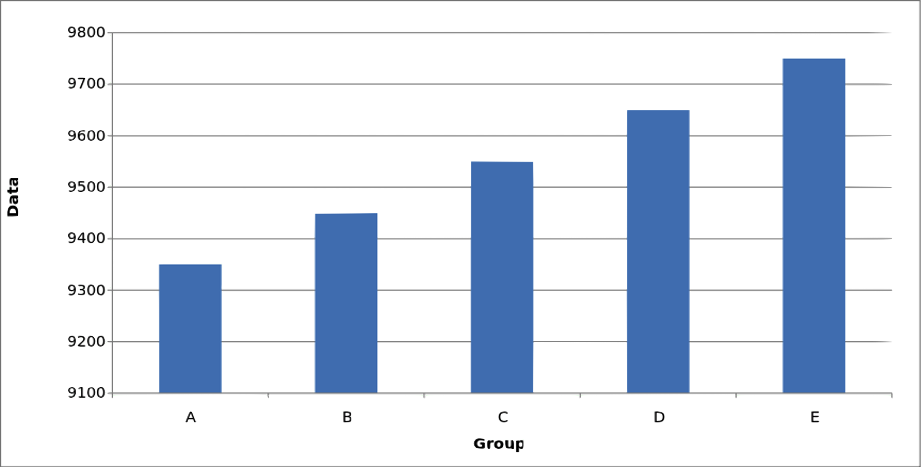
\includegraphics[width=.5\textwidth]{imagenes/imagenes01/T01IM32.png}
	\end{figure}
	
	\begin{figure}[H]
			\centering
			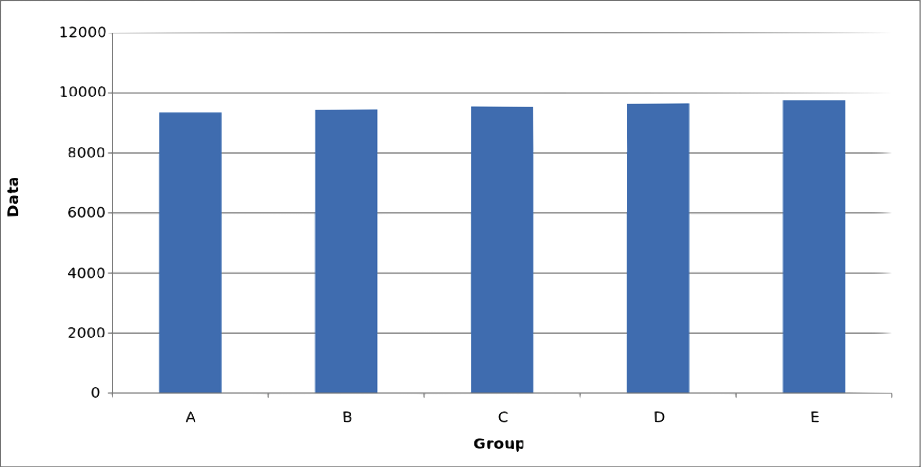
\includegraphics[width=.5\textwidth]{imagenes/imagenes01/T01IM33.png}
	\end{figure}
\end{multicols}


\begin{multicols}{2}
	\begin{figure}[H]
			\centering
			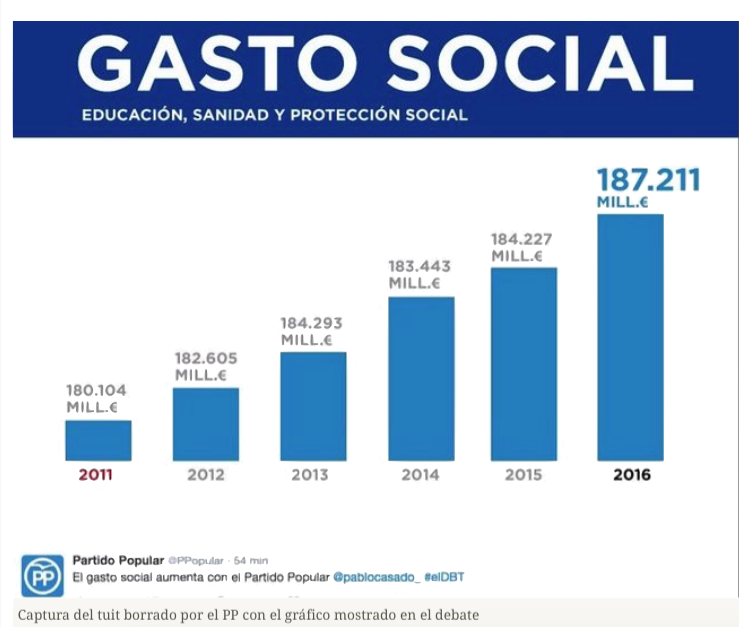
\includegraphics[width=.5\textwidth]{imagenes/imagenes01/T01IM34.png}
	\end{figure}
	
	\textcolor{white}{.}
	
	\begin{figure}[H]
			\centering
			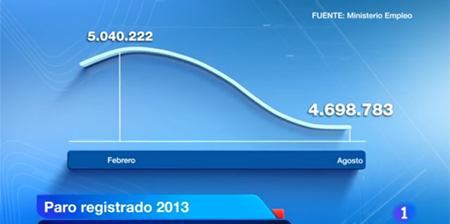
\includegraphics[width=.5\textwidth]{imagenes/imagenes01/T01IM35.png}
	\end{figure}
\end{multicols}



\vspace{2mm} Lo mismo ocurre con las secuencias de tiempo (habitualmente situadas en el eje X). El crecimiento o disminución de la delincuencia, economía, desempleo, IPC, etc. puede verse impresionante o irrelevante según qué período se tome. Habitualmente los políticos seleccionan los marcos de tiempo que mejor hacen ver su gestión.

\vspace{2mm} La próxima vez que veas uno de estos gráficos \emph{!`Asegúrate que partan de 0! O al menos, que consideren un marco de referencia suficientemente amplio para tener claro cuán relevante es la estadística}.

\vspace{2mm}  \textbf{3. Otras representaciones erróneas}

\vspace{2mm}  En el siguiente gráfico, a igualdad de frecuencia relativa para los sectores rojo y morado, el efecto 3D hace que al aparecer el sector morado más próximo al observador aumente su proporción respecto al sector rojo. También aumenta el efecto aparente de tamaño el hecho de extraer un sector de la tarta (el verde).

\begin{figure}[H]
			\centering
			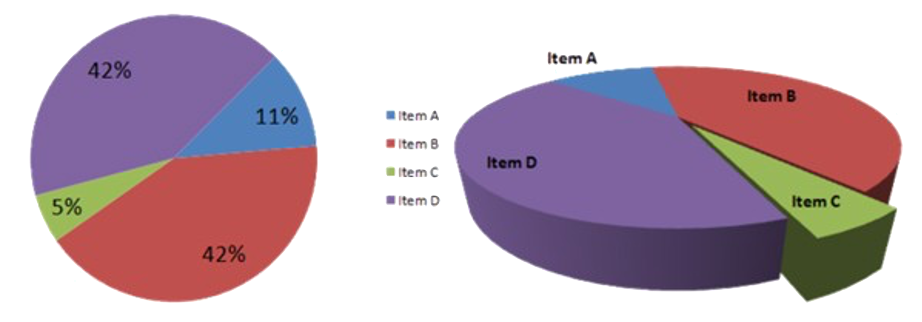
\includegraphics[width=.9\textwidth]{imagenes/imagenes01/T01IM38.png}
	\end{figure}

\vspace{2mm}  Uno de los más frecuentes errores de diseño en gráficos, y que ocurre hasta en los diarios y revistas más prestigioso, es usar dibujos con área o volumen, para representar un dato que debería tener un solo eje. Aunque se hace con un objetivo decorativo, el lector no sabe si debe comparar sólo la altura, el área o el volumen del objeto.

\begin{multicols}{2}
	\begin{figure}[H]
			\centering
			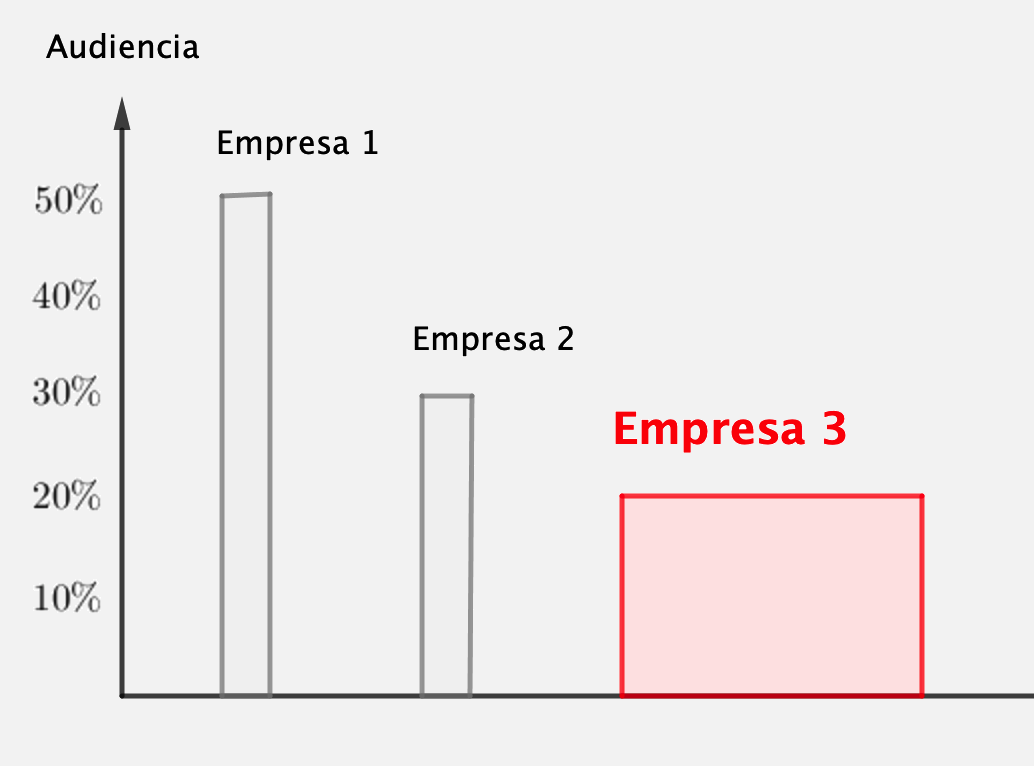
\includegraphics[width=.5\textwidth]{imagenes/imagenes01/T01IM36.png}
	\end{figure}
	
	\begin{figure}[H]
			\centering
			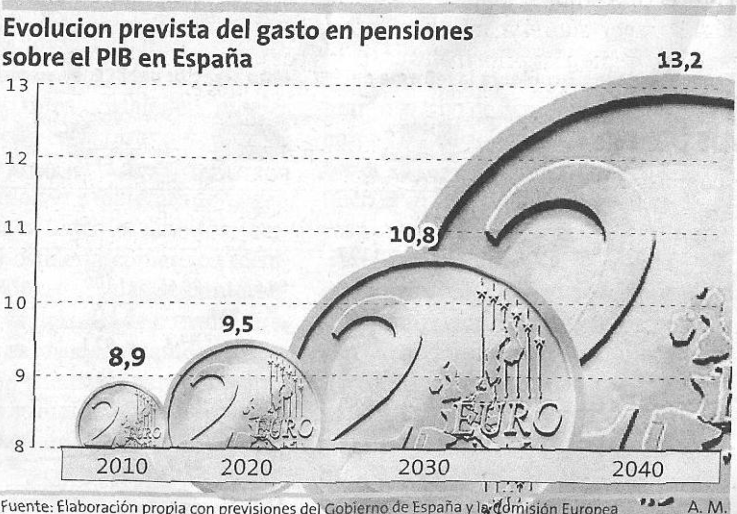
\includegraphics[width=.5\textwidth]{imagenes/imagenes01/T01IM37.png}
	\end{figure}
\end{multicols}


\vspace{2mm}  Aunque parezcan muchas cosas de las que estar preocupado, en realidad se trata de tener la misma actitud que frente a un estudio: \emph{ser escéptico}. En otras palabras, verificar que la fuente sea fiable (y que exista), que sus elementos tengan las proporciones correctas, y que la información que transmite (los números) sea la misma que nos dicen que transmite con los gráficos que la acompañan.


\end{myexampleblock}


\newpage

$\quad$

$\quad$



\begin{myblock}{RESUMEN Estadística descriptiva unidimensional}

$ \quad $

\begin{table}[H]
\centering
\begin{tabular}{c|c|c|c|c|c|c}
\hline
\multicolumn{1}{|c|}{$x_i$} & $n_i$ & $f_i$ & $N_i$ & $F_i$ & $x_i \cdot n_i$ & \multicolumn{1}{c|}{$x_i^2 \cdot n_i$} \\ \hline
\multicolumn{1}{|c|}{$\vdots$} & $\vdots$ & $\vdots$ & $\vdots$ & $\vdots$ & $\vdots$ & \multicolumn{1}{c|}{$\vdots$} \\ \hline
 & N & 1 &  &  & $\sum \to \bar x$ & $\sum \to s$
 
\end{tabular}
\end{table}
	
 $\triangleright \ $ Media(s):
  
 $$ \boxed{\ \bar x=\dfrac{\displaystyle \sum_{i=1}^n \ x_i \cdot n_i}{N} \ }
 \qquad  \quad
 \bar x_p=\dfrac{\sum x_i \cdot p_i}{\sum p_i} 
 \qquad \quad
 \bar x_g=\sqrt[N]{\prod x_i ^{n_i} } 
 \qquad \quad
 \bar x_a= \dfrac{N}{\sum \frac{x_i}{x_i}}$$
 
 \vspace{5mm} $\triangleright \ $ Moda:
 
 $$ mo\ = \ L_k + \dfrac{n_k-n_{k-1}}{(n_k-n_{k-1})+(n_k-n_{k+1})} \cdot c_k$$
 
 \vspace{5mm}  $\triangleright \ $ Mediana, Cuartiles, Deciles y Percentiles:
 
 $$me \ = \ L_k+\dfrac{ \frac N 2 + N_{k-1}}{n_k}\cdot c_k\ ; 
 \qquad  \qquad \qquad \qquad
 Q_i \ = \ L_k+\dfrac{i\cdot \frac N 4 + N_{k-1}}{n_k}\cdot c_k ;	\ \ i=1,2,3$$
 
 $$D_i \ = \ L_k+\dfrac{i\cdot \frac N {10} + N_{k-1}}{n_k}\cdot c_k ;	\ \ i=1,2,\cdots , 9 ; \qquad 
 P_i \ = \ L_k+\dfrac{i\cdot \frac N {100} + N_{k-1}}{n_k}\cdot c_k ;	\ \ i=1,2,\cdots , 99 $$
  
\vspace{5mm}  $\triangleright \ $ Varianza y desviación típica: 

$$ s^2 \ = \ \dfrac{\displaystyle \sum_{i=1}^n\ (x_i-\bar x)^2\cdot n_i}{N} \ = \ \dfrac{\sum x_i^2\cdot n_i}{N} - \bar x^2
\qquad \qquad \qquad \qquad 
s \ = \ \sqrt{s^2} $$

\vspace{5mm}  $\triangleright \ $ Coeficiente de variación (Pearson) y tipificación: 

$$ CV \ = \ \dfrac {s}{\bar x}
\qquad \qquad  
z_i \ = \ \dfrac {x_i-\bar x}{s}$$

$ \quad $

\end{myblock}

	